\chapter{ \label{chapter:il2} Methods to assess cell response to ex-vivo stimulation in flow cytometry }
%\chapter{ \label{chapter:il2} Effect of IL-2 Stimulation on Cell Phenotypes } 
%\chapter{ \label{chapter:il2} A recursive partitioning approach of identifying cells responsive to ex-vivo stimulation in flow cytometry }


\section{Background}

\Glspl{GWAS} have identified \cytokine{IL-2} signalling as a major aetiological pathway associated with the development of T1D.  
%The protective rs12722495 haplotype was significantly associated with increase in CD25 expression on CD4 memory T cells measured in terms of MFI.
%Howevever the protective combined rs2104286 genotype led to a decrease in the percentage of CD25 positive CD4 naive T cells.  
Disease associated \gene{IL2RA} variants in healthy individuals predict a decrease in expression of \protein{CD25},
the alpha chain of the trimeric \protein{IL-2} receptor, on memory \protein{CD4}\positive T lymphocytes \citep{Dendrou:2008gc,Dendrou:2009dv}.
As supported by an increase in soluble CD25, this process might be caused by preferential cleavage of the CD25 receptor.  
Regulatory and memory \protein{CD4}\positive T cells in healthy individuals with disease associated \gene{IL2RA} variants also exhibit decreased sensitivity to \cytokine{IL-2},
measured in terms of \protein{pSTAT5} activation \citep{Garg:2012jr}.
Disease associated variants of the phosphatase \gene{PTPN2}, a signaling molecule, also show diminished ability to respond to \cytokine{IL-2} \citep{Long:2011hk}.
Furthermore it is also suspected that \cytokine{IL-2} production might be diminished in T1D since disease associated variants in the \gene{IL2RA} correlate with
reduced \cytokine{IL-2} production \citep{Dendrou:2009dv}.
%really?
It has also been postulated that individuals with T1D have a reduced ability to respond to IL-2 due to multiple genetic defects in the IL-2 signalling 
pathway \citep{Long:2010ej}.
%IL-2 sensitivity drives IL-2 stimulation
%Defects in IL-2R signaling contribute to diminished maintenance of FOXP3 expression in CD4 positive CD25 positive regulatory T-cells of type 1 diabetic subjects 
%Preliminary data also suggests that the sensitivity to IL-2, measured in terms of pSTAT5 activation, may be also be reduced in the regulatory CD4+ T cells of newly diagnosed T1D patients.
%Furthermore it is also suspected that IL-2 production might be diminished in T1D
%since disease associated variants in the \emph{IL2RA} and \emph{PTPN2} genotypes correlate with reduced IL-2 production (reference?). 

\contributor{Tony Cutler} set to repeat and extend these findings in a more refined approach.
He selected 22 long-standing diabetics and 28 controls from the Cambridge Bioresource, as well as 
30 newly diagnosed and 15 unaffected siblings from the \Gls{D-GAP} resource.  
Hence a total of 52 cases and 43 controls, of which, 11 recalled individuals (5 cases and 6 controls) from the Cambridge Bioresource.
%In order to test these hypotheses, we selected 21 long-standing diabetics and 30 controls from the Cambridge Bioresource,
%as well as  28 newly diagnosed and 14 unaffected siblings from DGAP.
%The nature of the resource allows more flexibility to recall patients of interest, i.e those with low IL-2 signalling potential, for more in depth analysis.

%We set to repeat and extend these findings in a more refined approach.
%To test this hypothesis, blood samples are taken from 21 type 1 diabetics and 30 healthy controls.

Blood samples were prepared and analysed by flow cytometry on day of collection.
Each sample was split into four aliquot of \SI{500}{\micro\litre}.
The first aliquot was left unstimulated.
The remaining three were stimulated ex-vivo for 30 minutes at four 10-fold increasing doses
of proleukin (a variant of \cytokine{IL-2}) at $0.1$, $10$ or \SI{1000}{\unit\per\micro\litre} respectively.
%\SI{1000}{\unit\per\micro\litre} respectively.
After a set stimulation time, the samples are stained on a set of core markers, not affected by IL-2 stimulation, CD4, CD25, CD45RA, FoxP3,
used to delineate different cell types, and a functional marker, pSTAT5, a signalling protein of the IL-2 signalling pathway
that is phosphorylated on IL-2 stimulation.
We analysed the samples individually with flow cytometry.

We address the following research questions relating to the pSTAT5 response in these samples:
\begin{itemize}
  %\item Can some individuals be classified as low/high responders?
  \item In the cell subsets identified by manual gating, is the response to IL-2 associated with case-control status or any other covariate? 
  \item Using automated methods, can we find other responsive cell subsets which are ignored by the manual gating?
\end{itemize}

Answering the first question will depend on the reproducibility of the response between cell-subsets within individuals,
and we will see if, as in \Cref{chapter:IL2RA}, normalisation can improve the reproducibility.


%Tony Cutler, Saleha Hassan, Marcin Pekalski will be involved in immune function assays.
%Louise Bell will be ethics liason.
%Statistical analysis will be carried out by a delegated member of the Statistics team.
%Demands on DIL infrastructure 
%Blood handling rooms, BD LSRII Fortessa machine.

%\subsection{Panels}

\begin{table}[h!]\footnotesize
  \centering
\begin{tabularx}{\textwidth}{lcccc}
\rowcolor{Gray}
Flurochrome     & T/NK Cells & CD4 T Cells & CD4/naive \\
Alexa Fluor 488 & pSTAT5 & pSTAT5 & pSTAT5 & pSTAT5  \\
Alexa Fluor 700 & CD4    & CD4    & CD4    & CD4     \\
APC             & CD25   & CD25   & CD25   & CD25    \\
Pacific Blue    & CD56   & CD45RA & CD45RA & CD45RA  \\
PE YG           & FOXP3  & FOXP3  & FOXP3  & FOXP3   \\
PE-Cy7 YG       & CD45RA &        & CD31   & CD56    \\
PerCP Cy5-5     & CD3    &        &        &         \\
Qdot 605        & CD8    &        &        &         \\
\end{tabularx}
\mycaption{table:IL2-panels}
{IL-2 stimulation assay antibody-fluorochrome panel}
{
The fluorochrome-antibody panels used in IL-2 stimulation.
}
\end{table}


%196 FCS files: 38 individuals, 10 of which are recalled

%\begin{table}[ht]
%\centering
%\begin{tabular}{lllllll}
  %\hline
         %& individual & pch & day1       & day2       & day diff \\
  %\hline
%1        & CB00165D   & a   & 2012-11-29 & 2013-03-07 & 98 \\
%2        & CB00366X   & b   & 2012-11-07 & 2013-03-27 & 140 \\
%3        & CB00396E   & c   & 2012-09-25 & 2013-03-11 & 167 \\
%4        & CB00406Q   & d   & 2012-10-16 & 2013-01-22 & 98 \\
%5        & CB01484M   & e   & 2012-09-25 & 2013-03-11 & 167 \\
%6        & CB01494Y   & f   & 2012-10-09 & 2013-01-29 & 112 \\
%7        & CB01495Z   & g   & 2012-10-09 & 2013-01-29 & 112 \\
%8        & CB01498C   & h   & 2012-10-16 & 2013-01-22 & 98 \\
%9        & CB01503H   & i   & 2012-11-07 & 2013-03-07 & 120 \\
%10       & CB01504J   & j   & 2012-11-07 & 2013-03-27 & 140 \\
   %\hline
%\end{tabular}
%\mycaption{table:IL2-recalled-individuals}
%{Ten individuals recalled between 98 and 168 days later. }
%{
%}
%\end{table}
%

\begin{table}[ht]
\centering
\begin{tabular}{lll}
  \hline
         &  pch & day diff \\
  \hline
1        &  a   & 98 \\
2        &  b   & 140 \\
3        &  c   & 167 \\
4        &  d   & 98 \\
5        &  e   & 167 \\
6        &  f   & 112 \\
7        &  g   & 112 \\
8        &  h   & 98 \\
9        &  i   & 120 \\
10       &  j   & 140 \\
   \hline
\end{tabular}
\mycaption{table:IL2-recalled-individuals}
{Ten individuals recalled between 98 and 168 days later. }
{
}
\end{table}




\begin{figure}
\centering
\includegraphics[scale=.5] {flowdatasets/figures/il2-stimulation-samples-time.pdf}
\mycaption{figure:IL2-sample-time} 
{ Days on which samples are processed. }
{
}
\end{figure}

\begin{figure}[h]
\centering
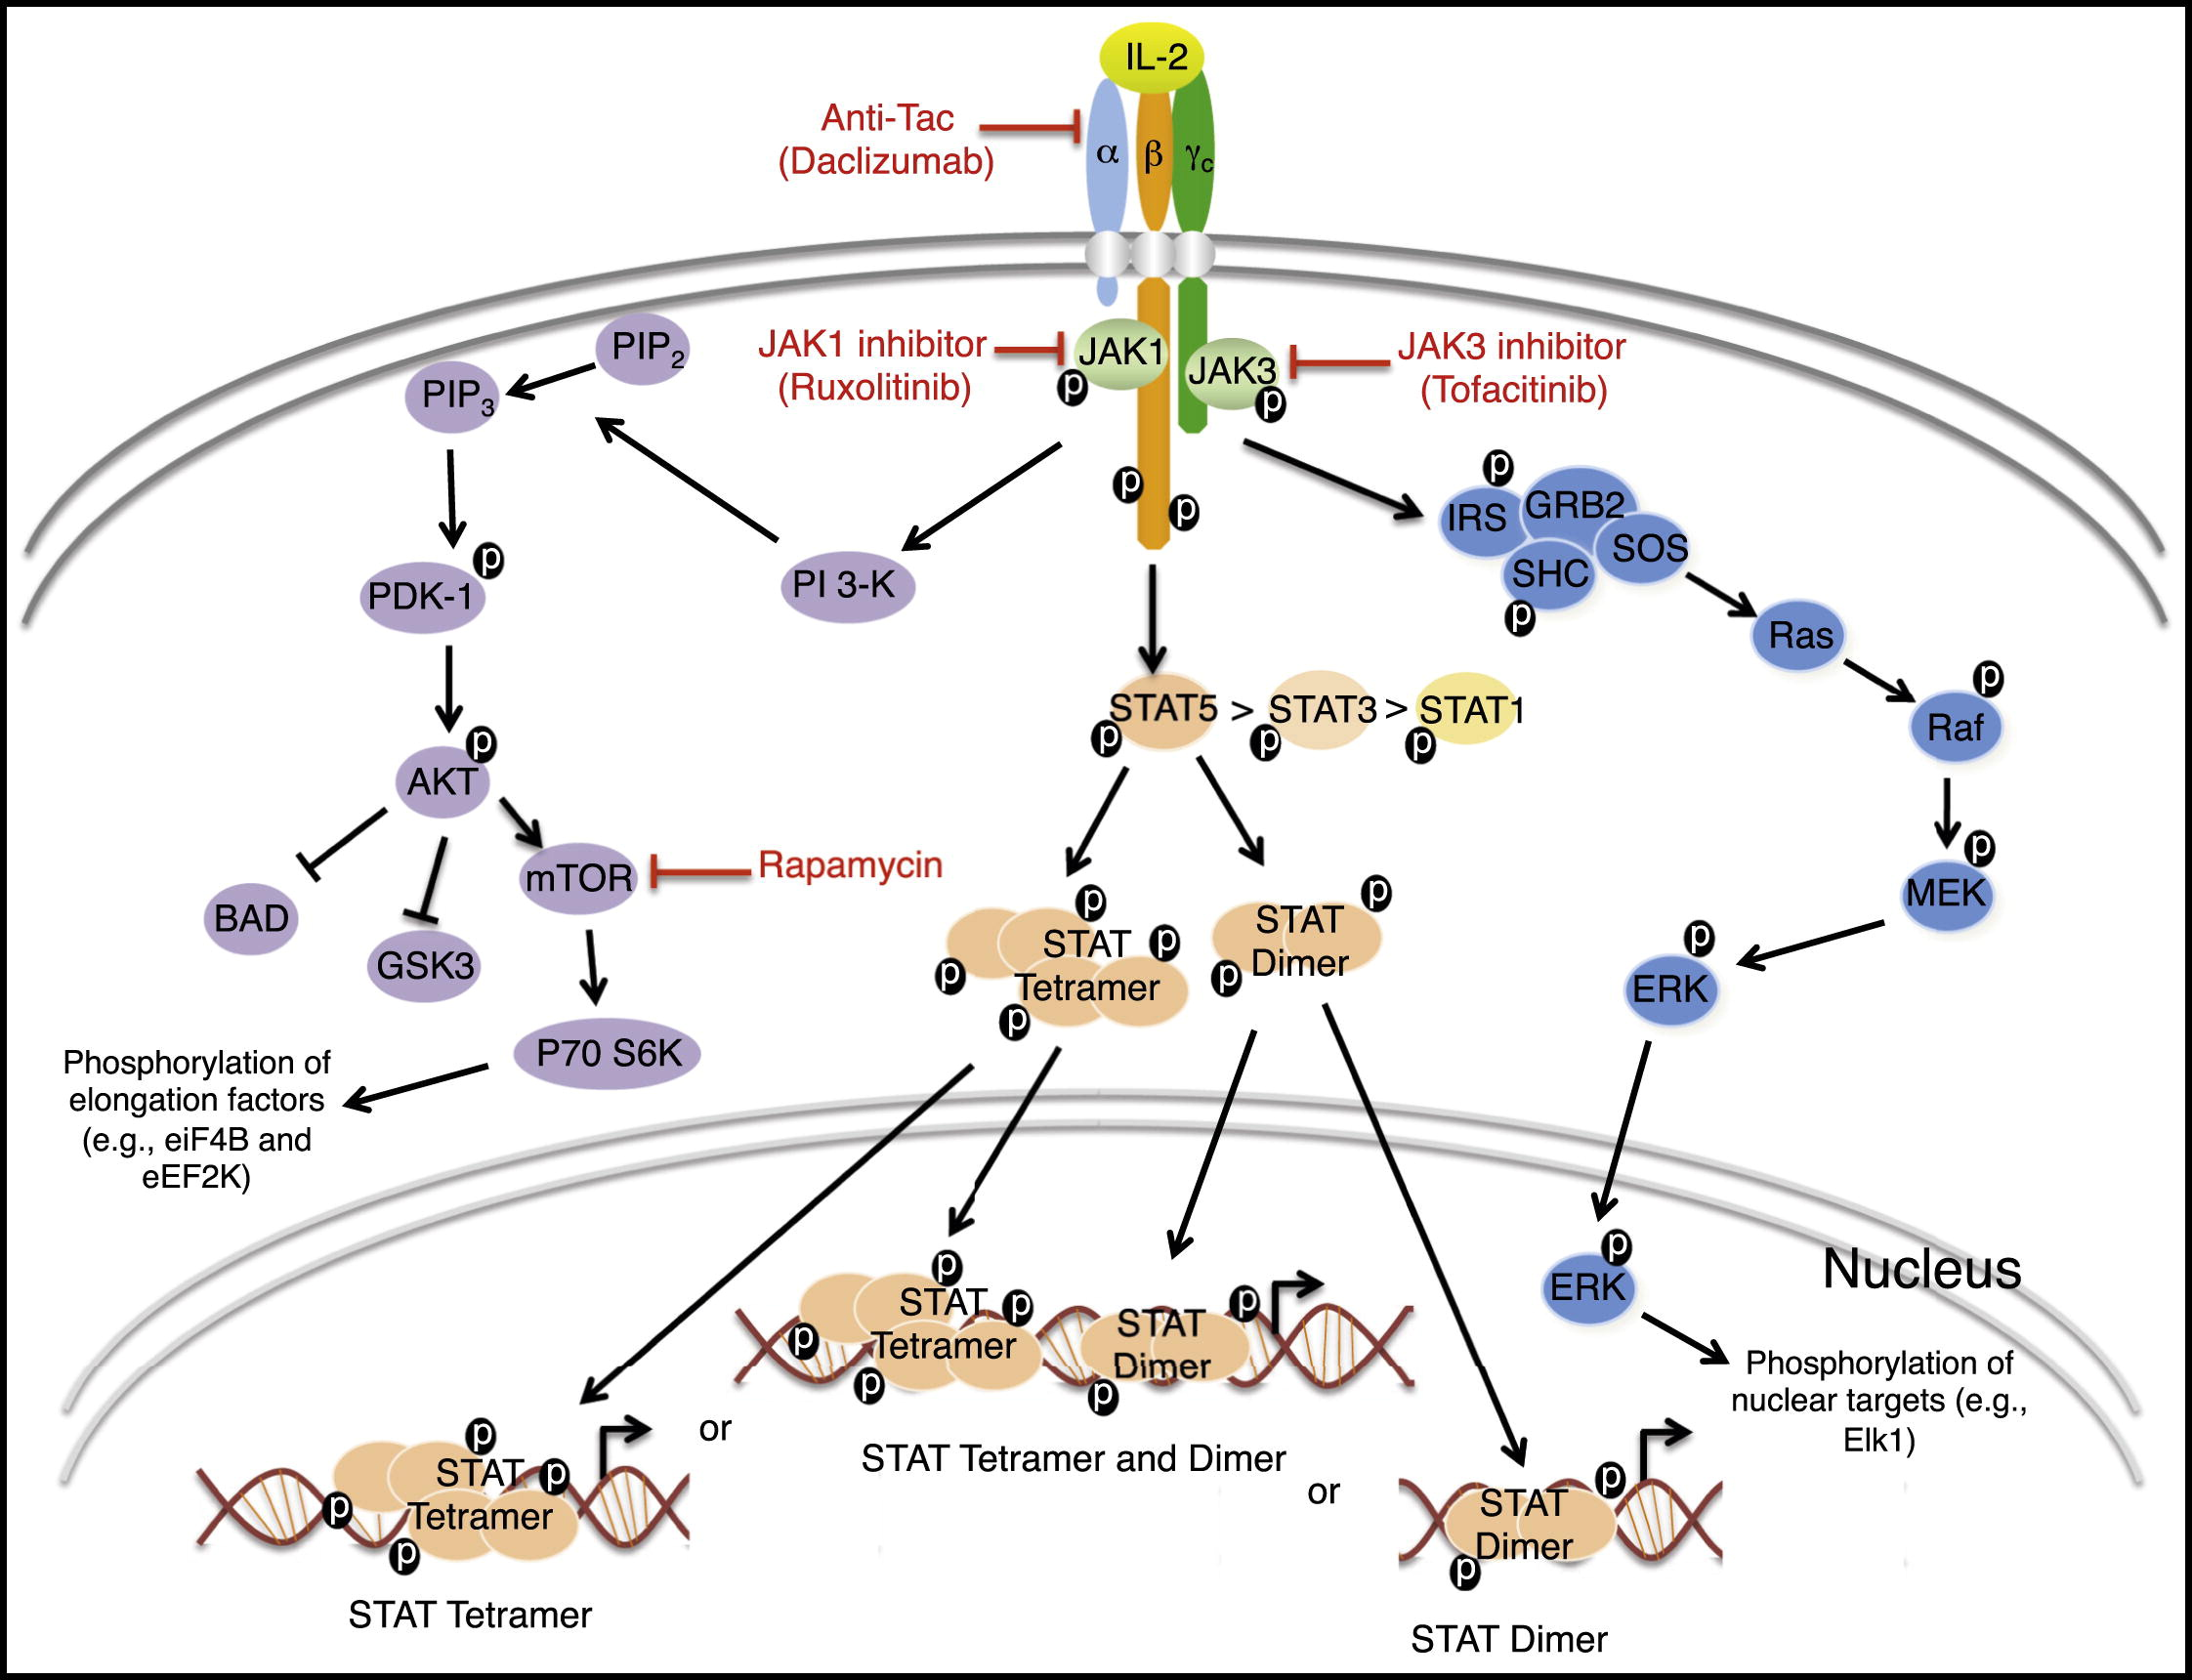
\includegraphics[scale=0.75]{IL2/figures/IL2-pathway.jpg}
\mycaption{figure:jones-2000}
{Figure from \citet{Liao:2013jt}.}
{
\protein{CD25} is \protein{IL2RA}, the $\alpha$ subunit of the trimeric \cytokine{IL-2} receptor.
The $\alpha$ is the highest binding affinity receptor of the three chains.
STAT5 is phosphorylated to pSTAT5 and acts as a transcription factor.
%Schematic of Major IL-2 Signaling Pathways
%Shown is the activation of PI 3-K-AKT, JAK-STAT, and SHC-RAS-MAPK signaling pathways. Also shown are potential therapeutic points of control for IL-2 signaling, with anti-Tac (daclizumab), rapamycin, and JAK1 or JAK3 inhibitors being shown in red. The cartoon shows signaling by both STATs dimers and tetramers. The figure indicates that IL-2 activates more STAT5 than STAT3 and more STAT3 than STAT1. ERK refers to both ERK1 and ERK2. MEK refers to both MEK1 and MEK2.
}
\end{figure}


\section{pSTAT response in the manually gated cell subsets}

%\section{Joining samples on core markers using approximate nearest-neighbour}

In order to facilitate the analysis, samples are first joined on their core markers using the \gls{ANN} to the resting sample \citep{Jones:2011ez}
as implemented in the \Rpackage{RANN}.
This creates a dataset of the same number of cells as the resting dataset, but where each cell now has a total of four functional pSTAT5 markers,
one for each stimulation dose.
At each cell it is now possible to assess the difference in pSTAT5 response between resting and stimulated.
This is important because all cells do not have the same resting level of pSTAT5 (\Cref{figure:pstat5-beaseline-relative}).
This approach presents a number of advantages.
Firstly, only the sample to which the other samples are joined needs to be gated.
Secondly, since the pSTAT5 response is relative to the baseline, it should be more robust to day variation
and consequently, more reproducible than pSTAT5 fluorescence intensity.
Thirdly, since we have response at the cell-level, we can use methods
such as \gls{CART}, \gls{RF} and \gls{MARS} to do multivariate regression of pSTAT5 from core markers.
This could help identify cells which would have been missed from only examining core markers.
%which will investigate in the second section.

%An alternative to this approach, would be to gate subsets in subsamples stimulated at different doses and subtract the background,
%however a clear advantage of this approach is that it allows for methods such as RF and MARS

The \gls{ANN} approach is valid without normalisation since the distributions of the core markers align across doses (\Cref{figure:core-markers}).
\Cref{figure:ann-join-0U-01U} confirms that the mapping of the clusters is correct across the nearest-neighbour mapping.

%When the between-dose variation on the core markers is negligeable,
%If we assume that the within-tube variation is negligeable, then a simpler solution is possible:
%each cell in the unstimulated subsample is joined to its closest neighbouring cell (in terms of its core markers) in a stimulated subsample.
%This assumes that the core markers are fairly stable across samples, which is usually the case in ex-vivo stimulated.



%The joining results is also not affected by any euclidean distance preserving transform, so the FCS data can be transformed before or after the \gls{ANN} joining.
%Another important check is to see whether the joining is sensitive to the transform.
%We find that we get the same results whether we join before or after the transform.


\hspace{-2cm}
\begin{figure}[h]
\centering
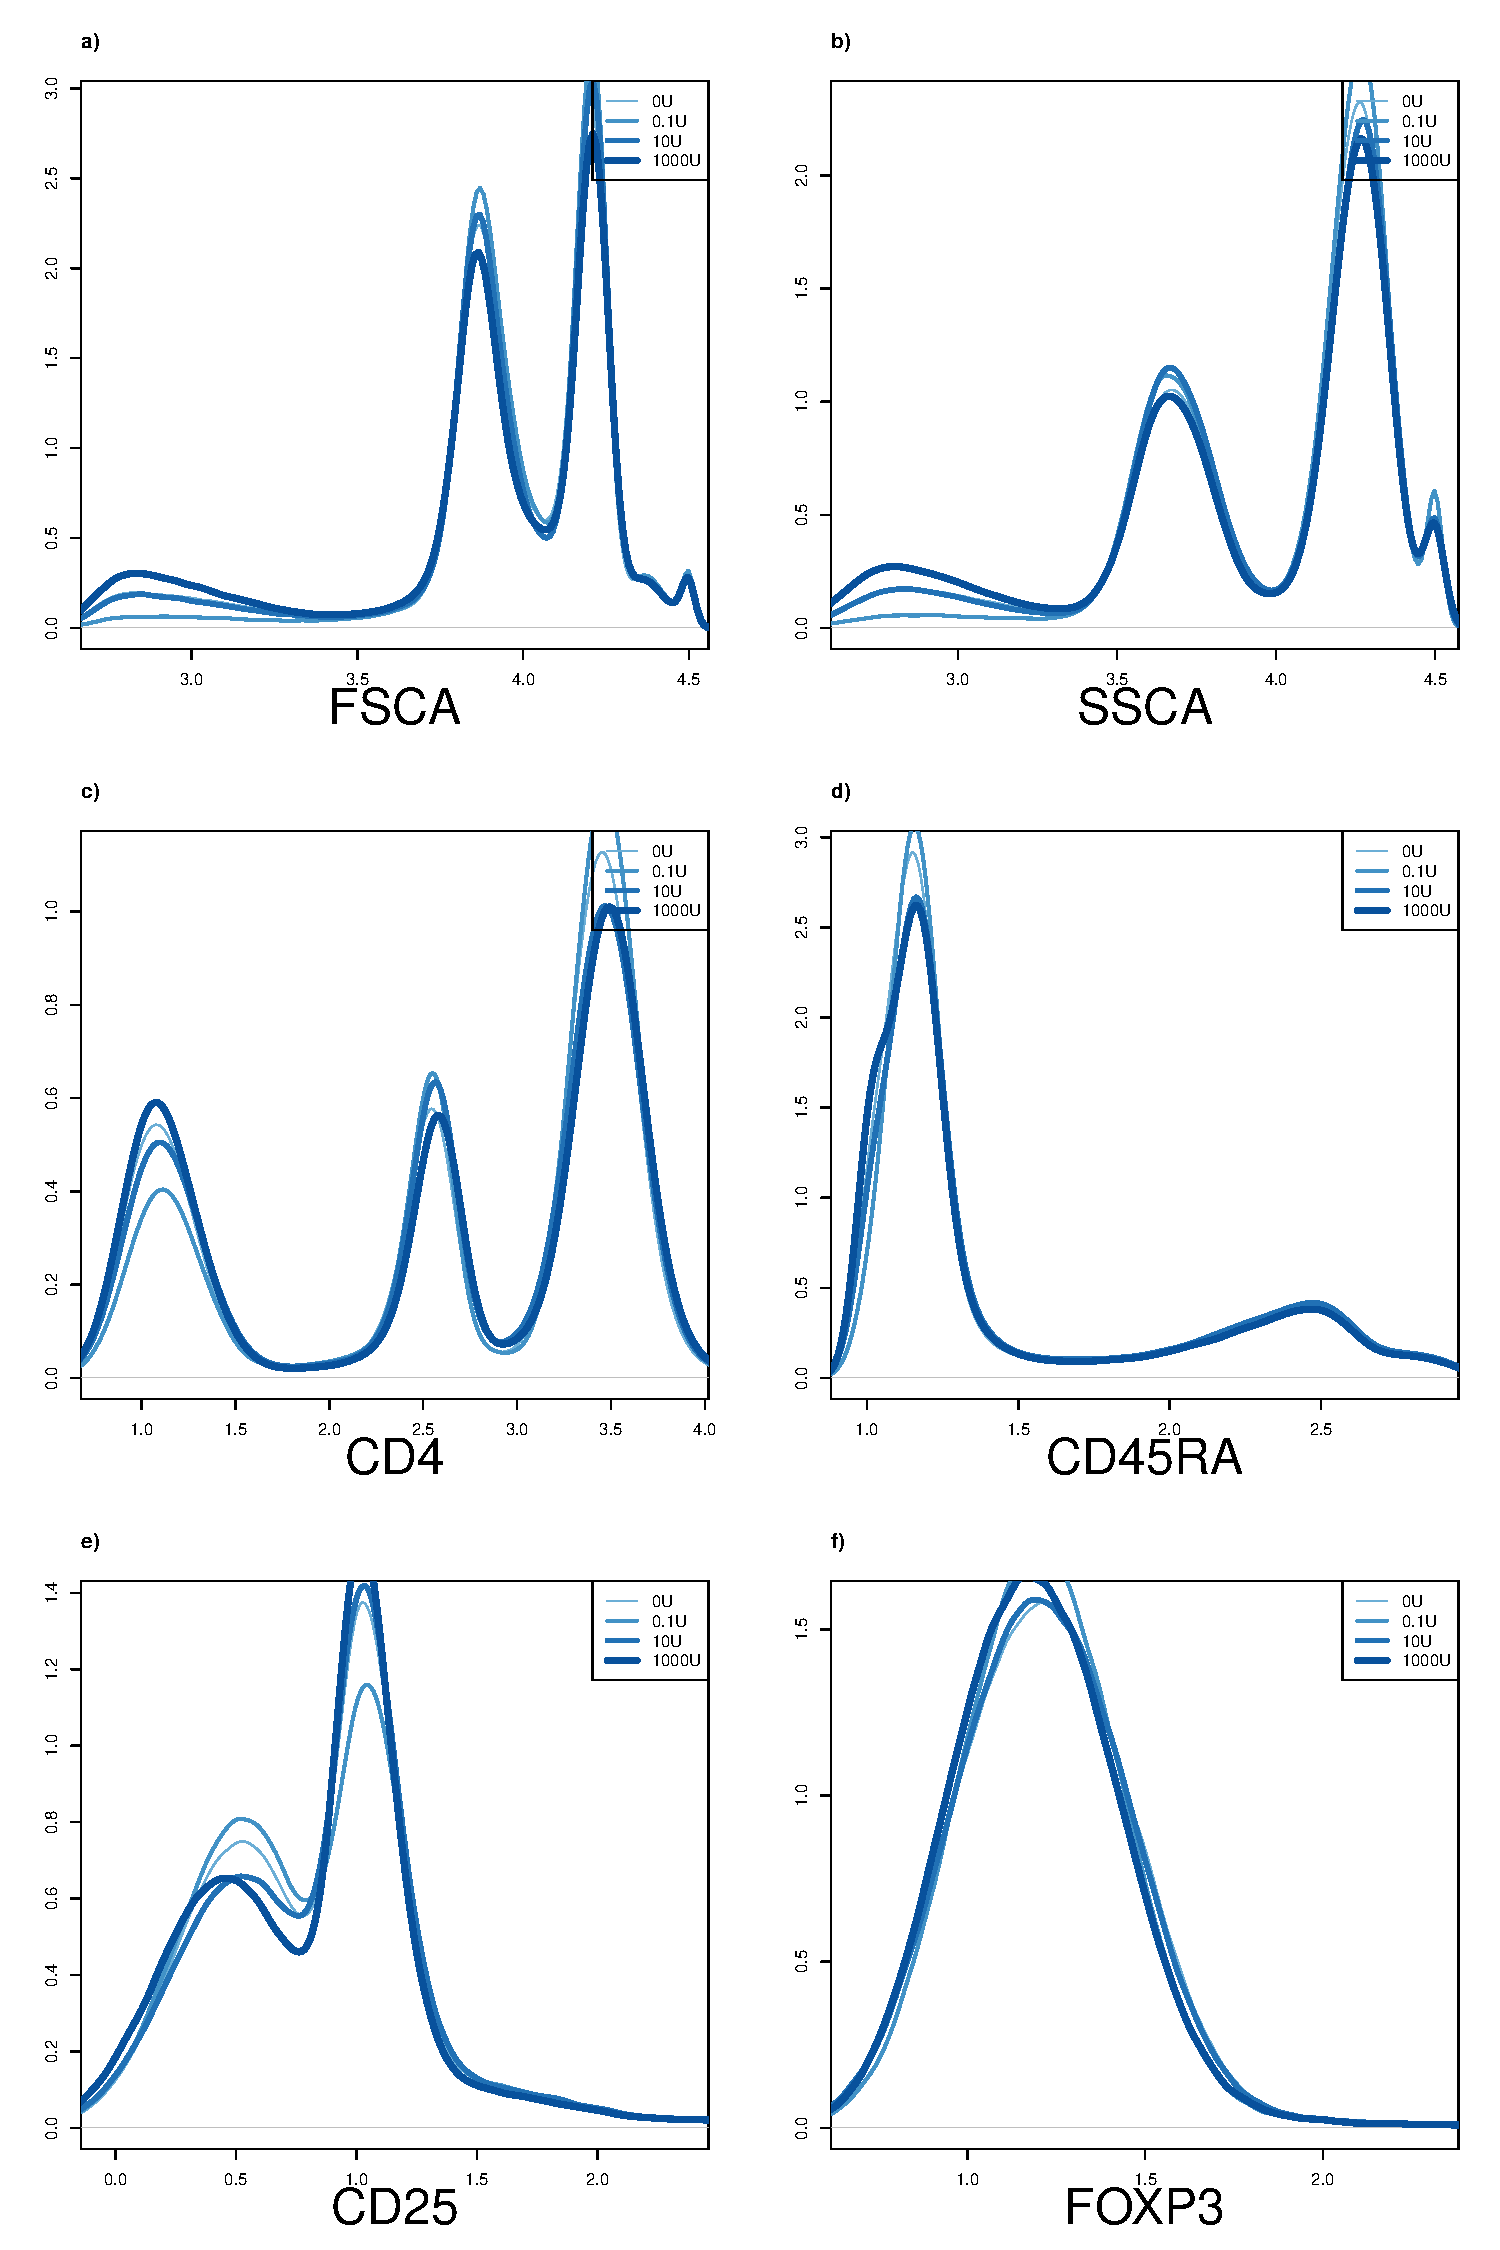
\includegraphics[scale=.3]{IL2/figures/dose-effect.pdf}
\mycaption{figure:core-markers}
{Dose-effect on core markers in ungated sample.}
{
Increasing doses represented by lines of increasing thickness.
The distributions align well across doses.
}
\end{figure}

\hspace{-2cm}
\begin{figure}[h]
\centering
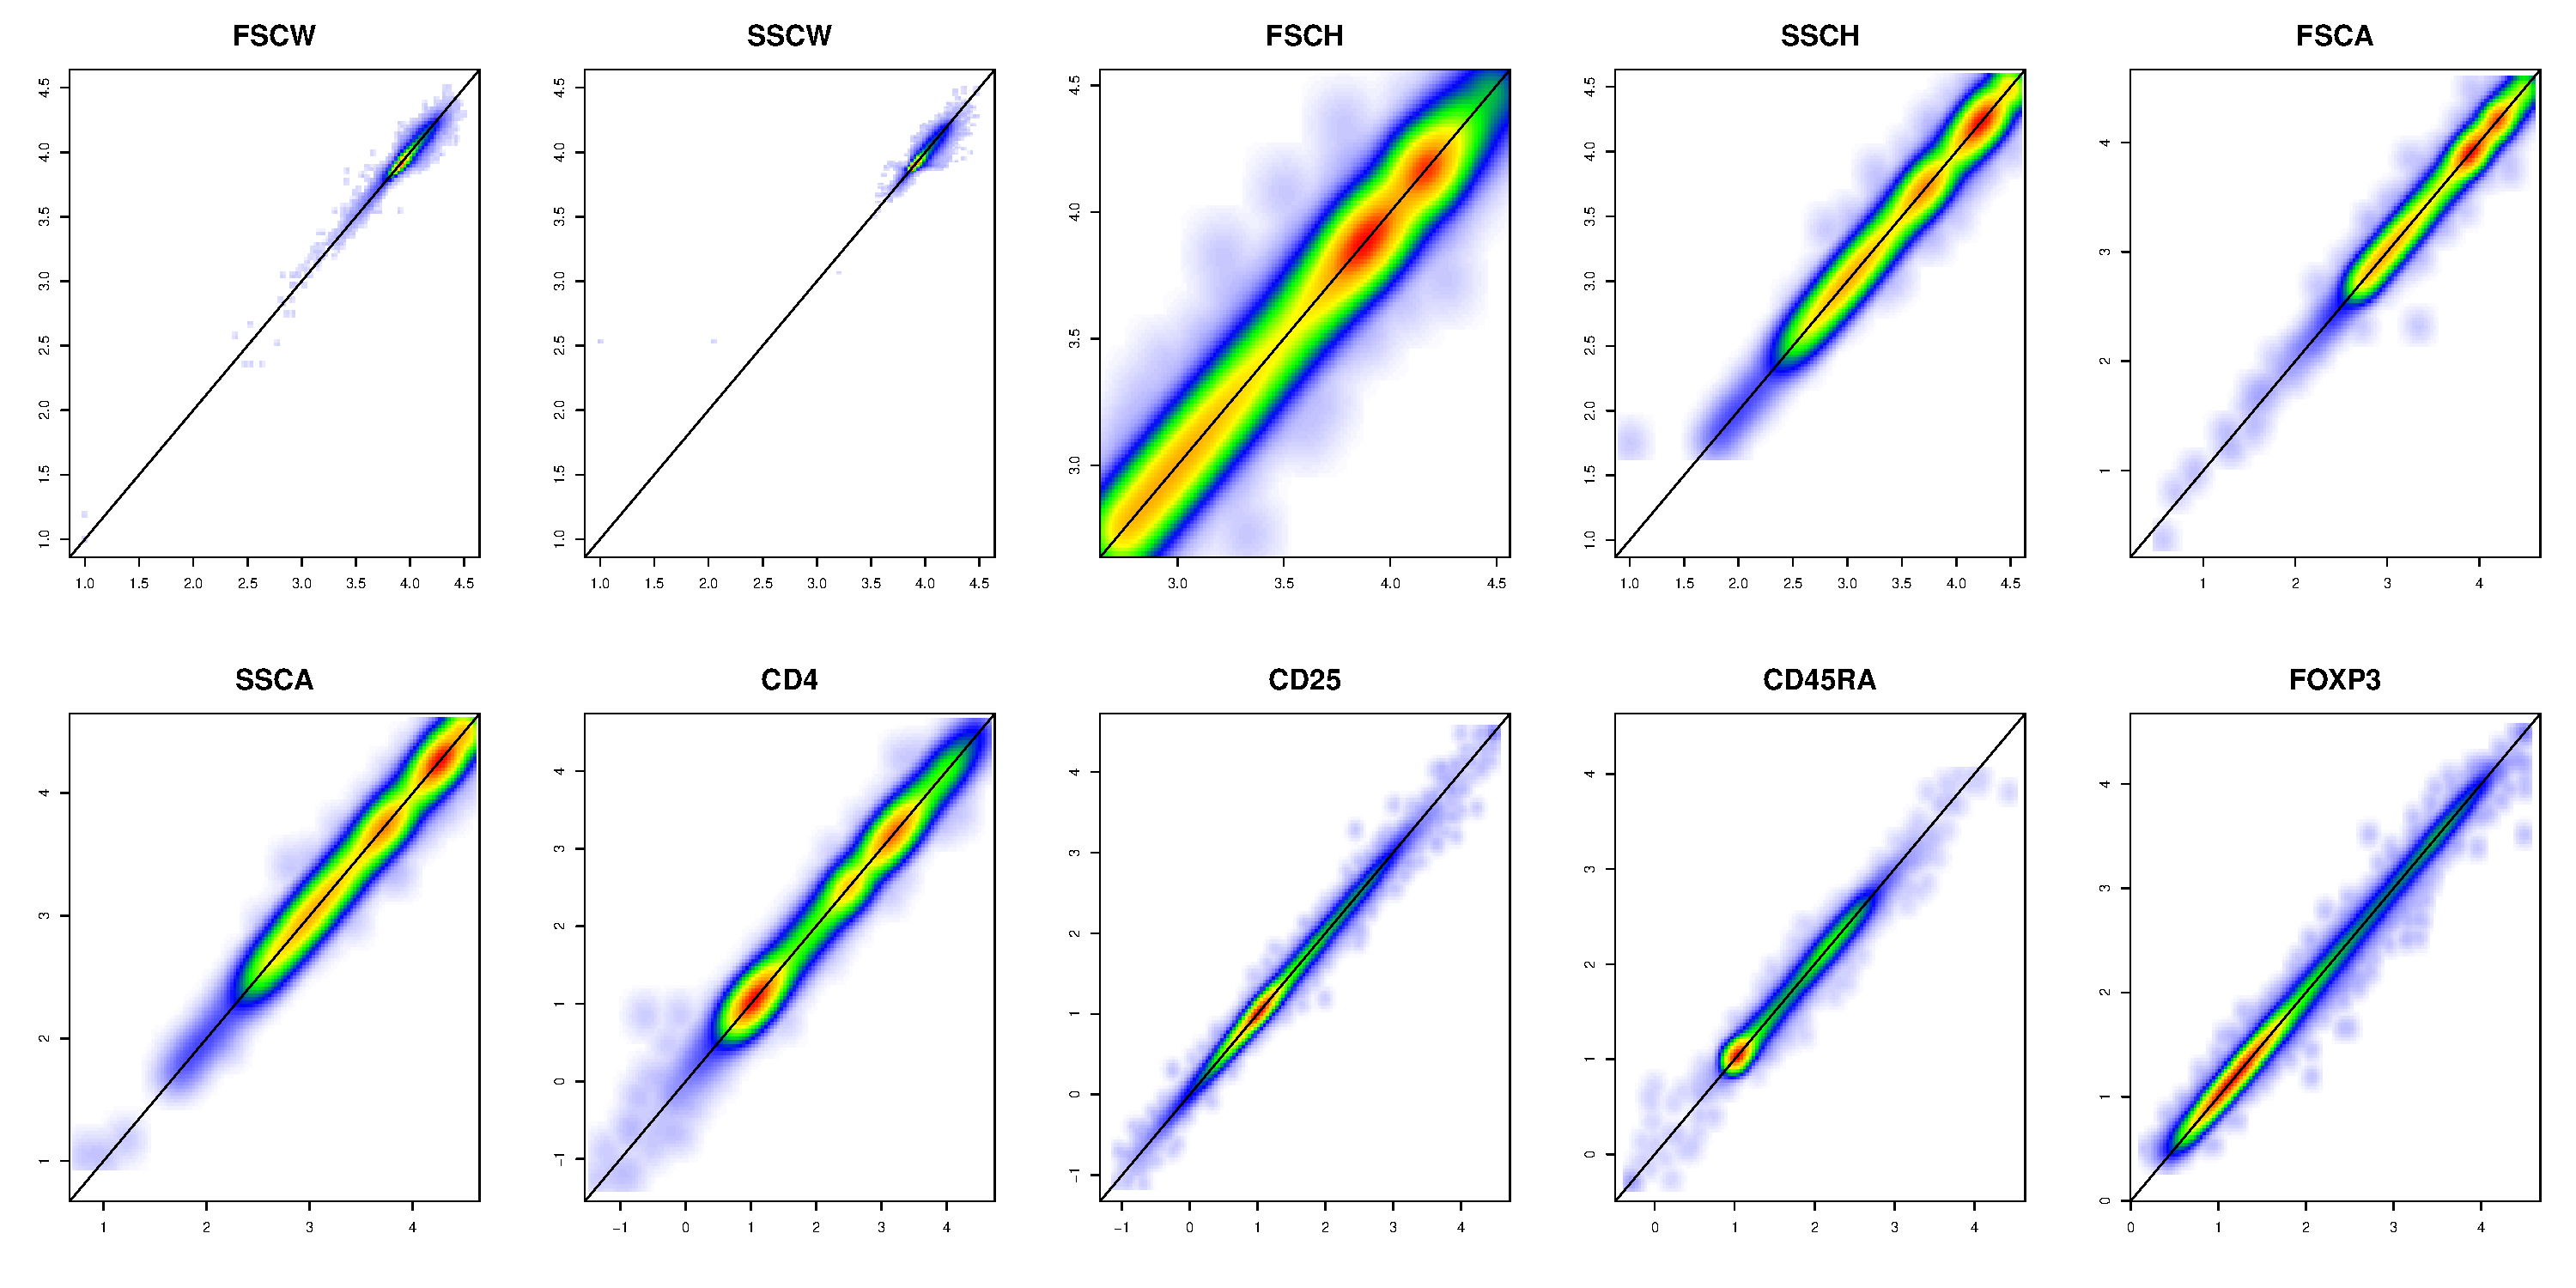
\includegraphics[scale=.3]{IL2/figures/ann-join-0U-01U.pdf}
\mycaption{figure:ann-join-0U-01U}
{Nearest neighbour join on core markers of ungated resting sample with ungated sample stimulated at 0.1 units. }
{
All clusters lie on the y=x line which suggests that clusters are correctly matched across samples.
}
\end{figure}


\hspace{-2cm}
\begin{figure}[h]
\centering
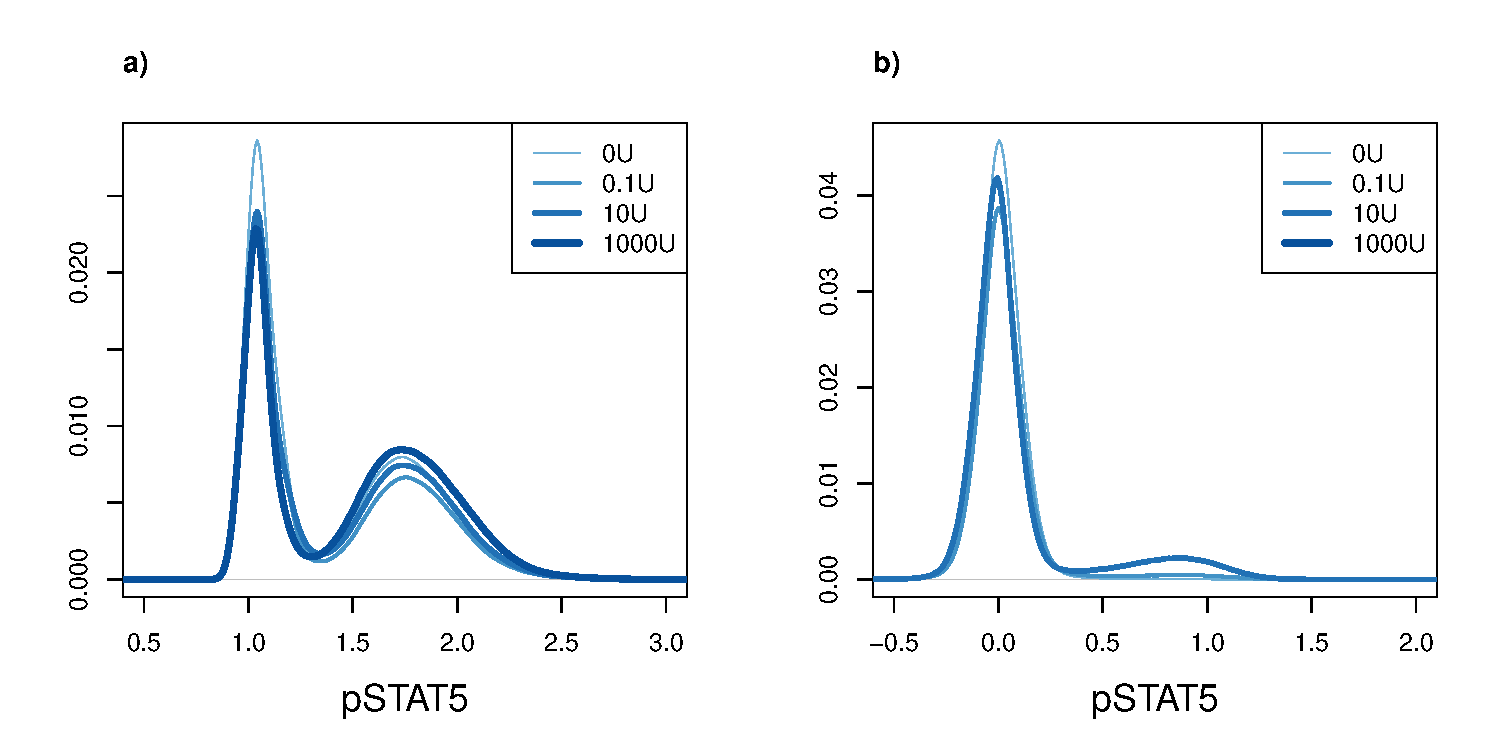
\includegraphics[scale=.5]{IL2/figures/pstat5-baseline-relative.pdf}
\mycaption{figure:pstat5-baseline-relative}
{ pSTAT5 intensity across the four proleukin doses, before (a) and after (b) baseline pSTAT5 subtraction in the ungated sample.}
{
  An important proportion of cells are already saturated for pSTAT5 (high baseline) in the resting sample (a).
  Correcting for the per cell pSTAT5 baseline, shows the true proportion of cells which responds to proleukin within this sample (b).
}
\end{figure}




\section{Cell Phenotypes Identified by Manual Analysis}


In the preliminary manual analysis using FlowJo conducted by \contributor{Tony Cutler}, pSTAT5 activation was assessed in terms of MFI and percent pSTAT5 positive according
to the proportion of pSTAT5 positive cells above the unstimulated control for each individual subset of lymphocytes tested.  
%The pSTAT5 distribution was measured in effector and regulatory naive and memory T cell populations (Figure~\ref{figure:tony-cd4-gating}).
Manual gating focused on four lymphocyte subsets(\Cref{figure:tony-cd4-gating}):
\begin{itemize}
  \item memory effector
  \item memory treg
  \item naive effector
  \item naive treg
\end{itemize}
Within each subset, the pSTAT5 distribution was measured at the four proleukin doses (\Cref{figure:dose-effect-pstat5-cellsubsets}).
As expected, the distributions shifts to the right as more STAT5 is phosporylated at higher doses of proleukin.
Of the four subsets, the most sensitive cells to proleukin are the memory and naive regulatory T cells (\Cref{figure:dose-effect-pstat5-cellsubsets} b and d),
then the memory effector (\Cref{figure:dose-effect-pstat5-cellsubsets} a) and finally the naive effector (\Cref{figure:dose-effect-pstat5-cellsubsets} c).
The sensitivity of the response in these cell subsets is confirmed by plotting of dose against MFI (\Cref{figure:pstat5-response-cellsubsets}).
This also illustrates that pSTAT5 saturation occurs in naive and memory regulatory T cells at 10 units or proleukin while naive effector cells do not reach
saturation even at the highest dose of 1000 units.
%Defining a threshold for pSTAT5 positivity is done using a similar approach as in \Cref{chapter:il2ra}.
%The top percentile of the pSTAT5 distribution in the resting sample is used as a threshold as described in %\Cref{ }.
 
%Some individuals with a reduced pSTAT5 response consistent across studied cell types were identified by Tony, however there was no evidence of association with disease status.  

%There are unsolved day to day variation issues, better to do in bulk from frozen once Foxp3 IC stain works
%A question of potential interest with whether the low responders show any other immunological phenotype such as for example Th17, IL-21 production, Tfh proportion?

%\begin{figure}[h]
    %\centering
    %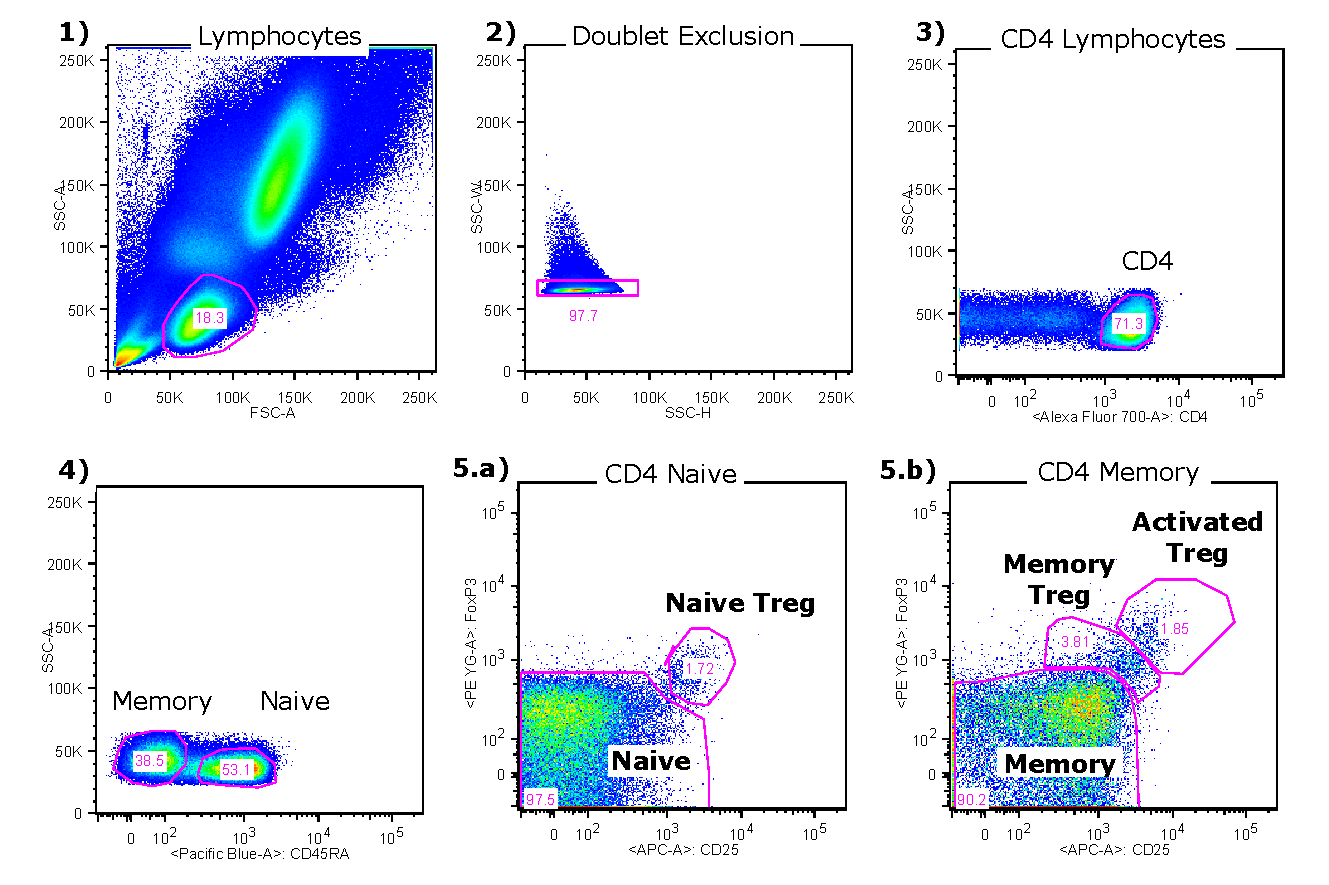
\includegraphics[scale=.75]{IL2/figures/tony-cd4-gating.pdf}
    %\caption{  \label{figure:tony-cd4-gating} Manual gating conducted by \contributor{Tony Cutler} to identify:
    %conventional and regulatory naive and memory T cells as well as activated regulatory T cells.
    %}
%\end{figure}
%

\hspace{-2cm}
\begin{figure}[h]
\centering
%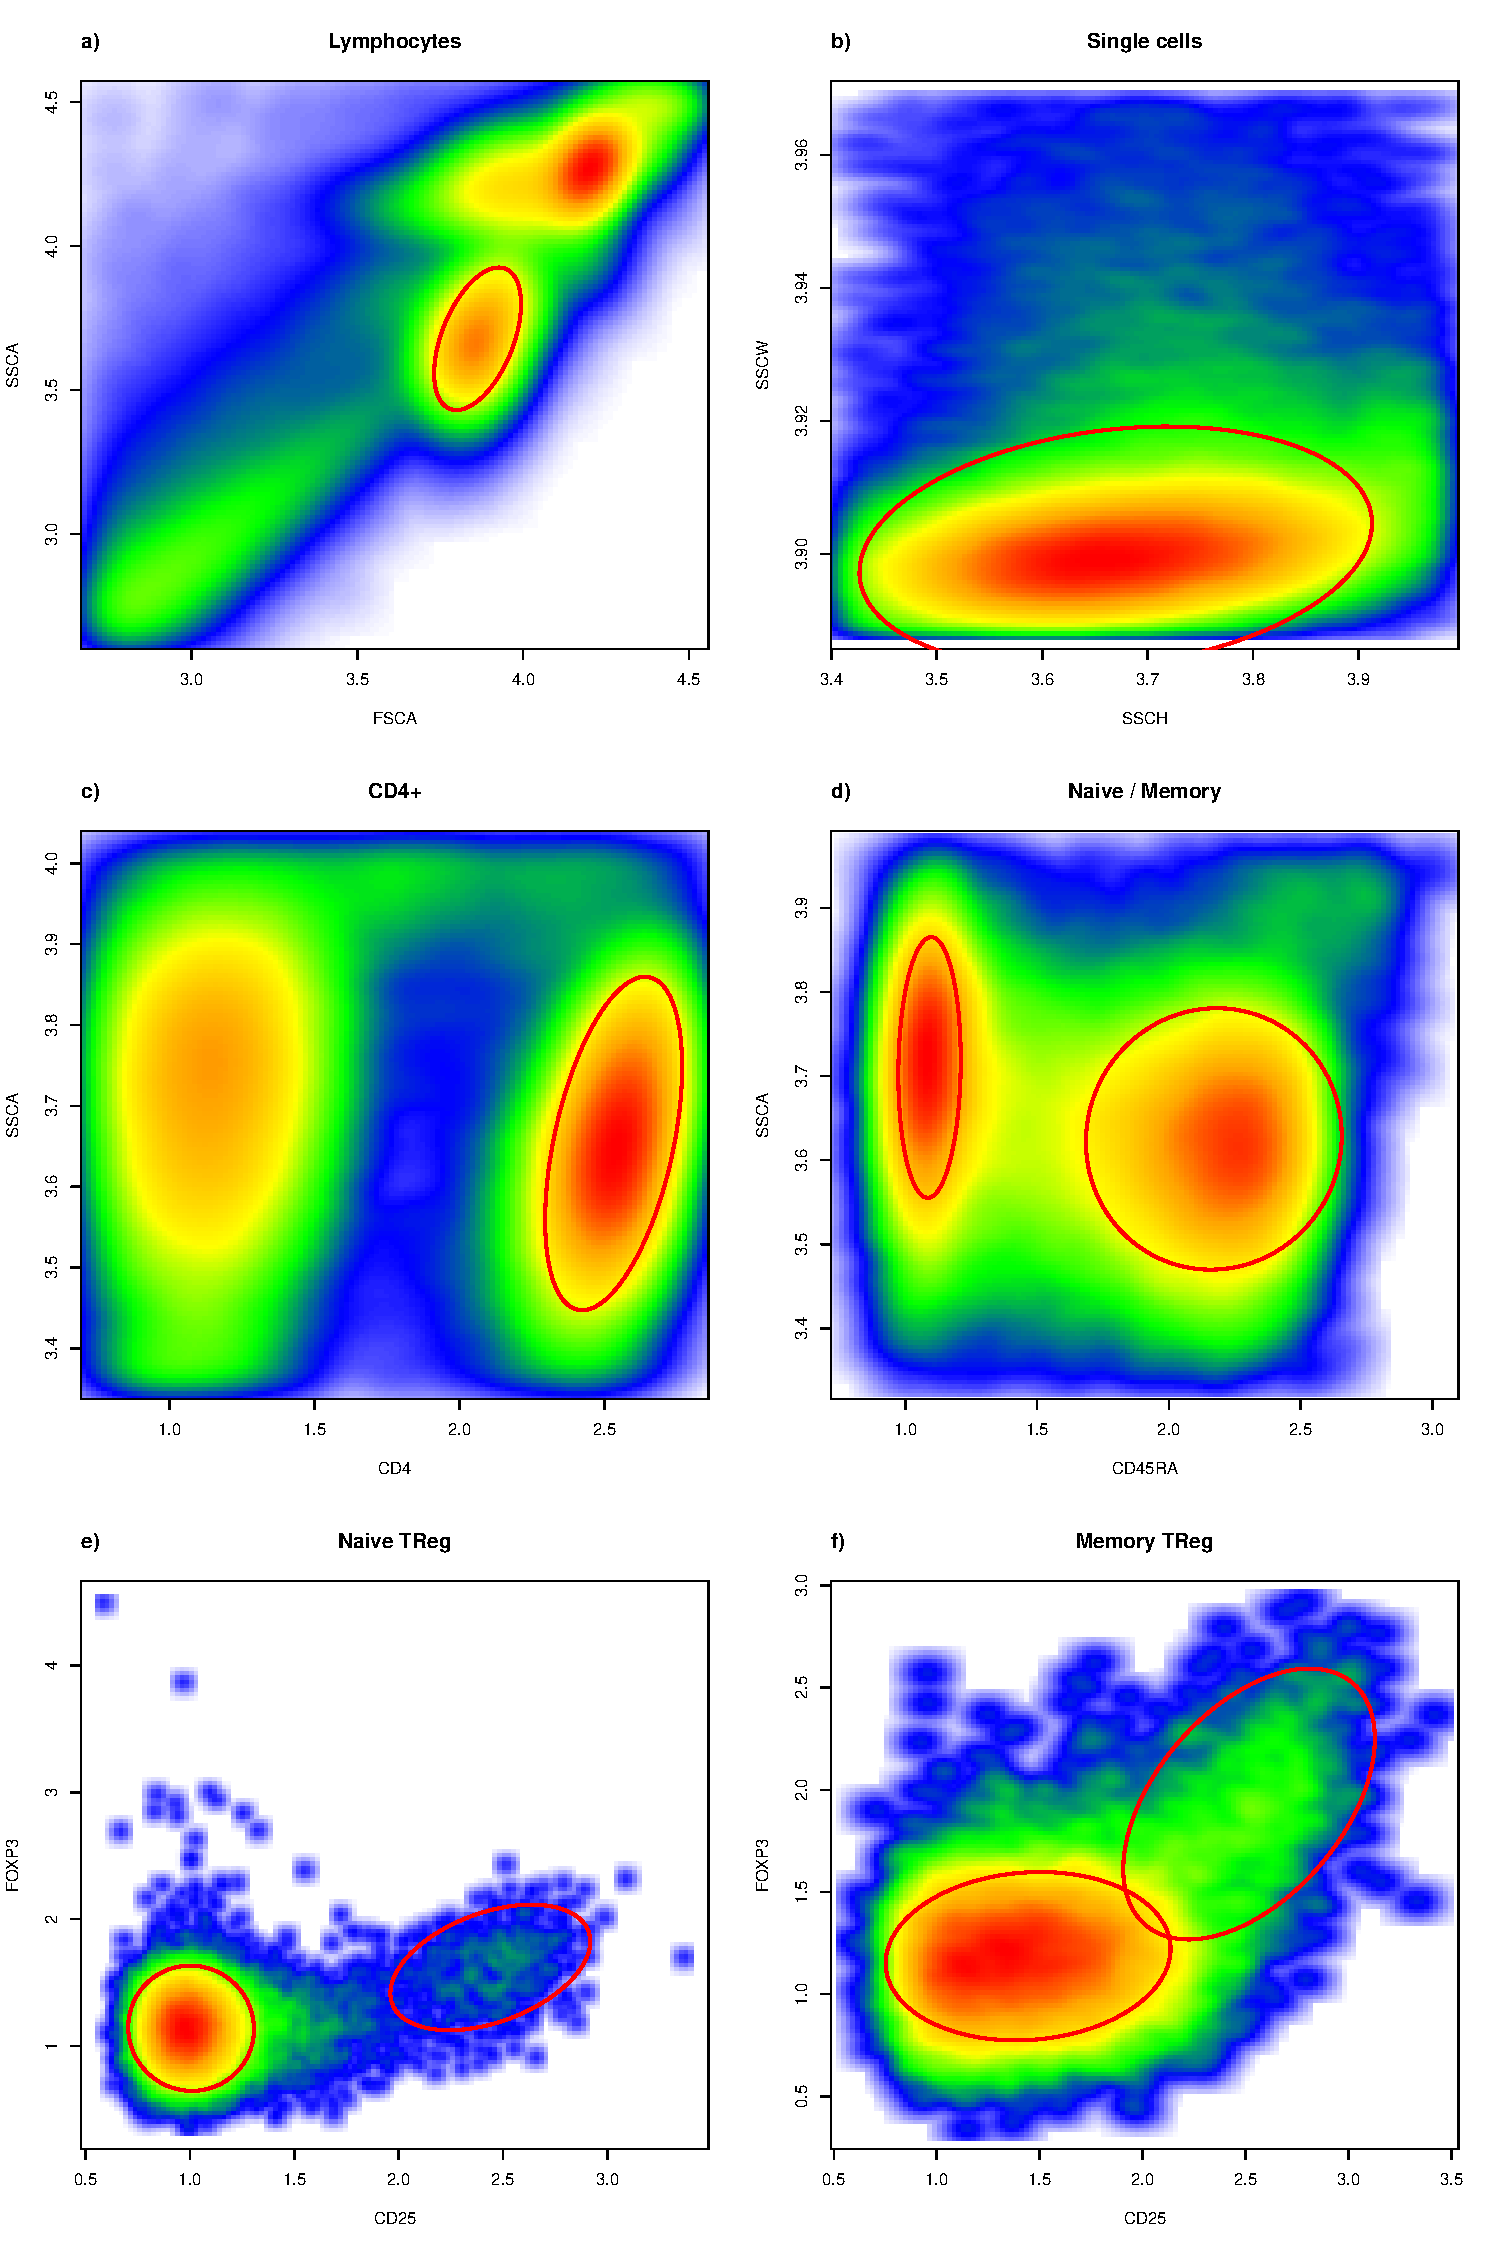
\includegraphics[scale=.5]{figures/manual-gating.pdf}
%\begin{subfigure}[b]{.4\textwidth}
%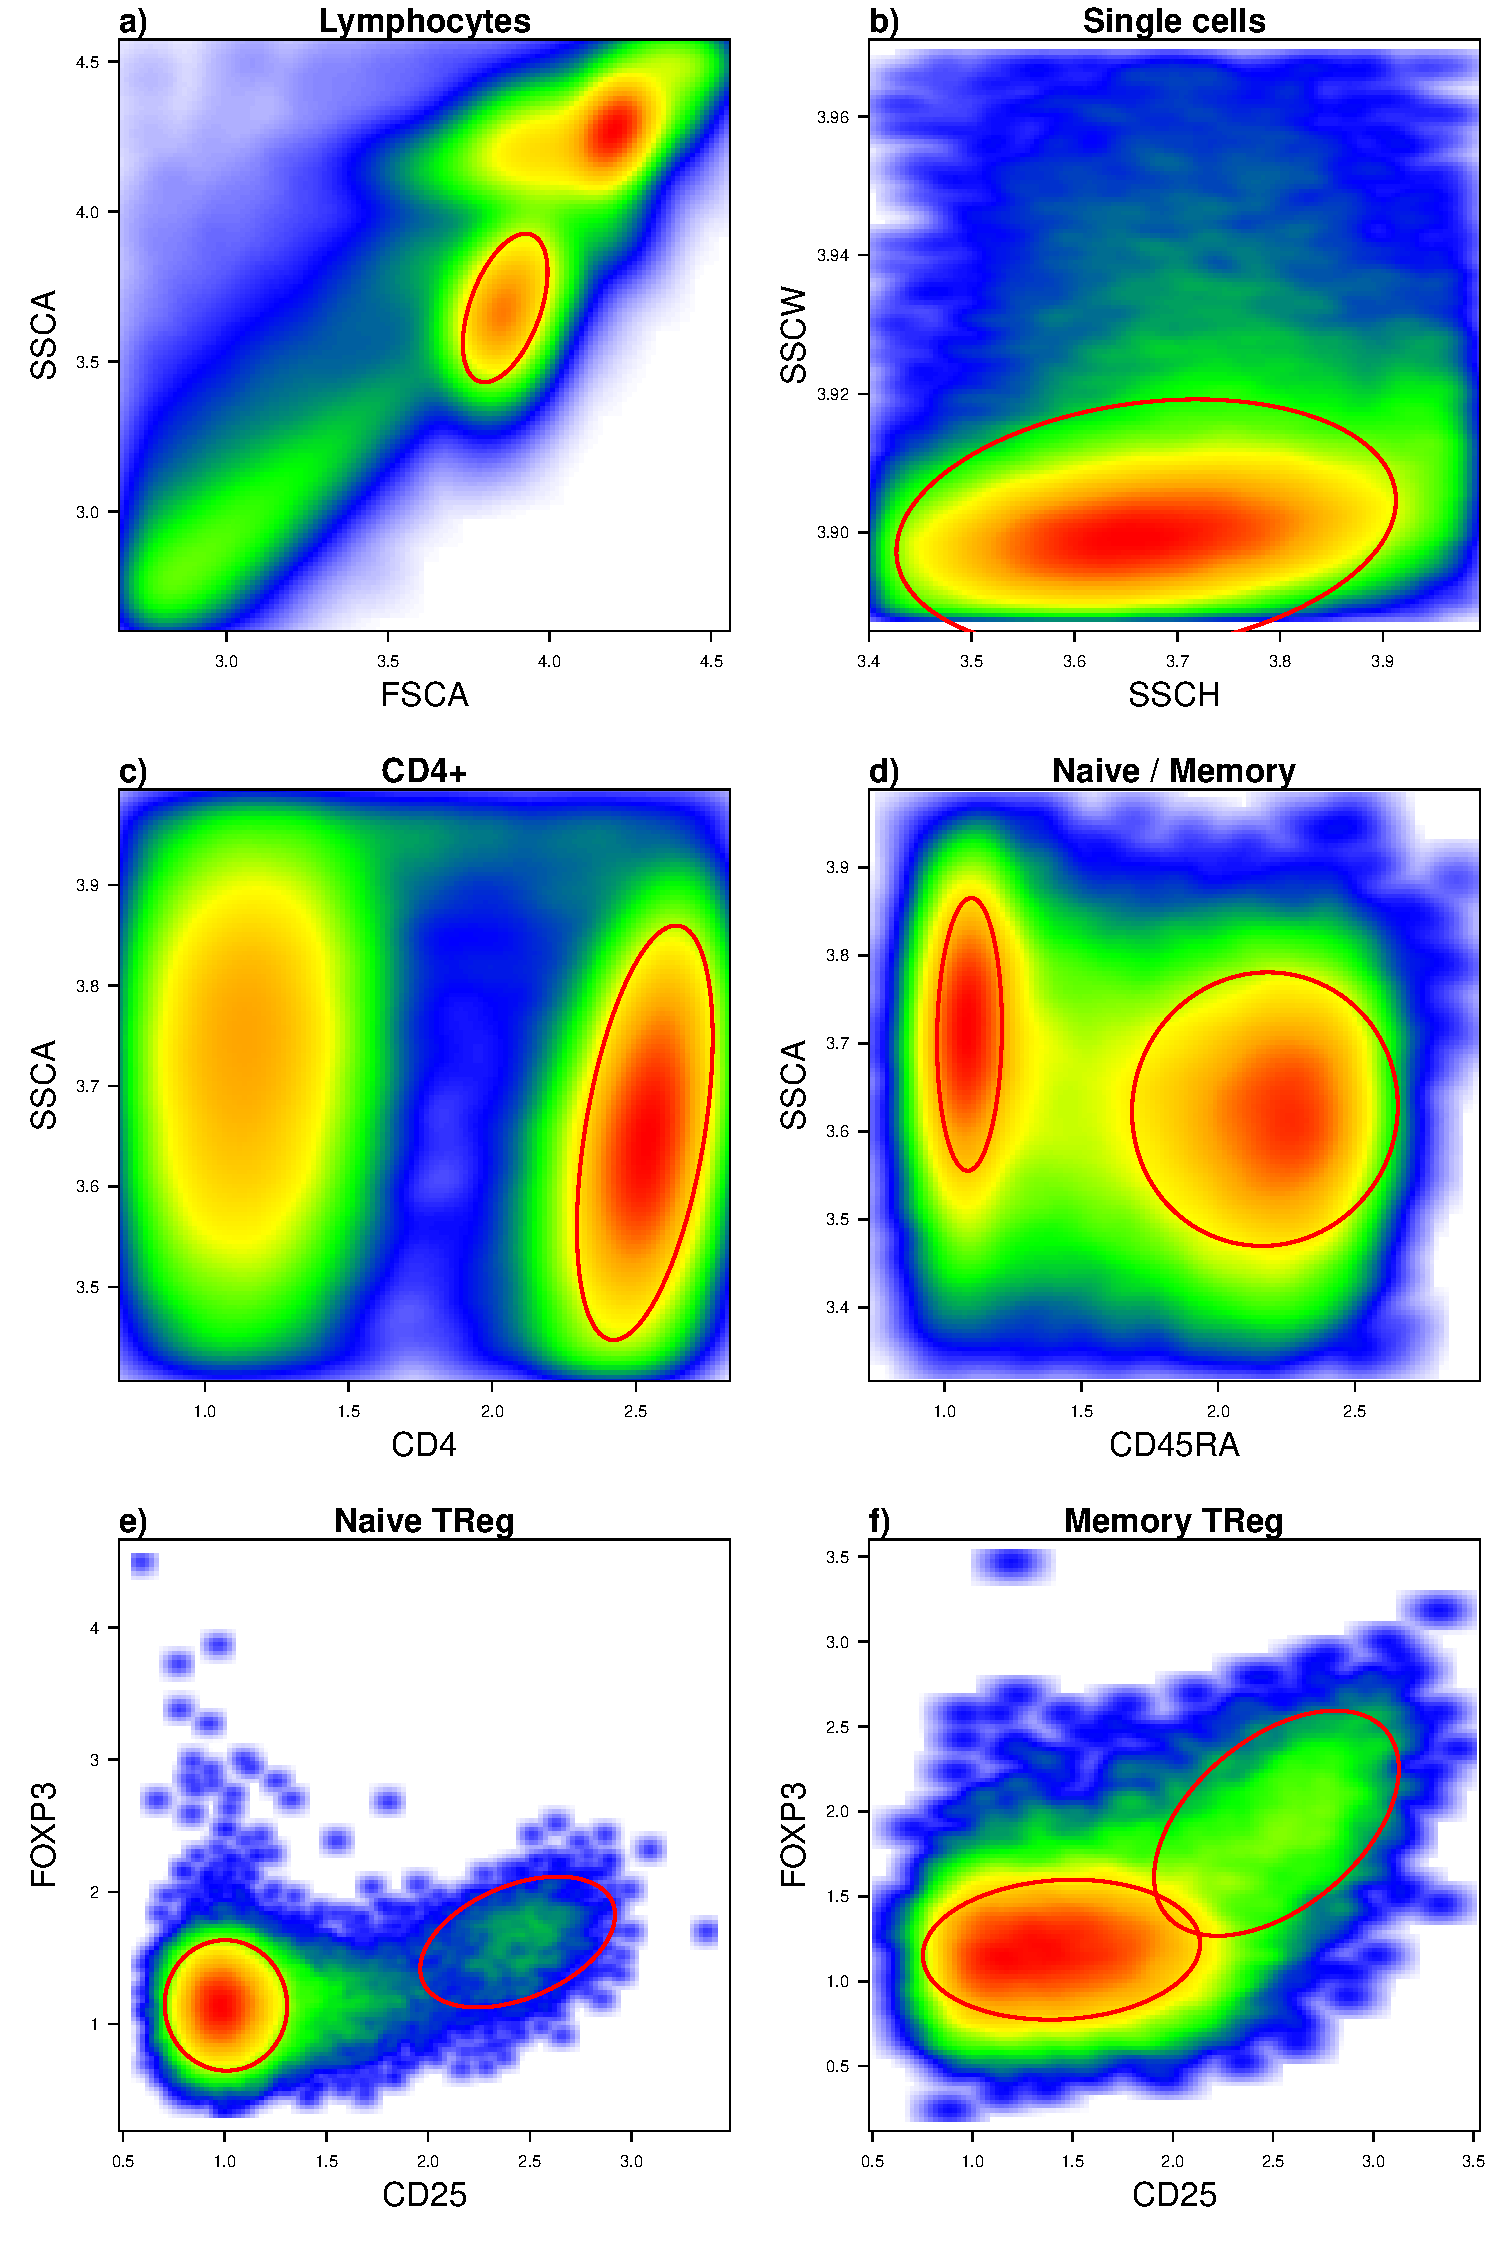
\includegraphics[scale=.25]{IL2/figures/manual-gating-CB00165D_0U_2012-11-29.pdf}
  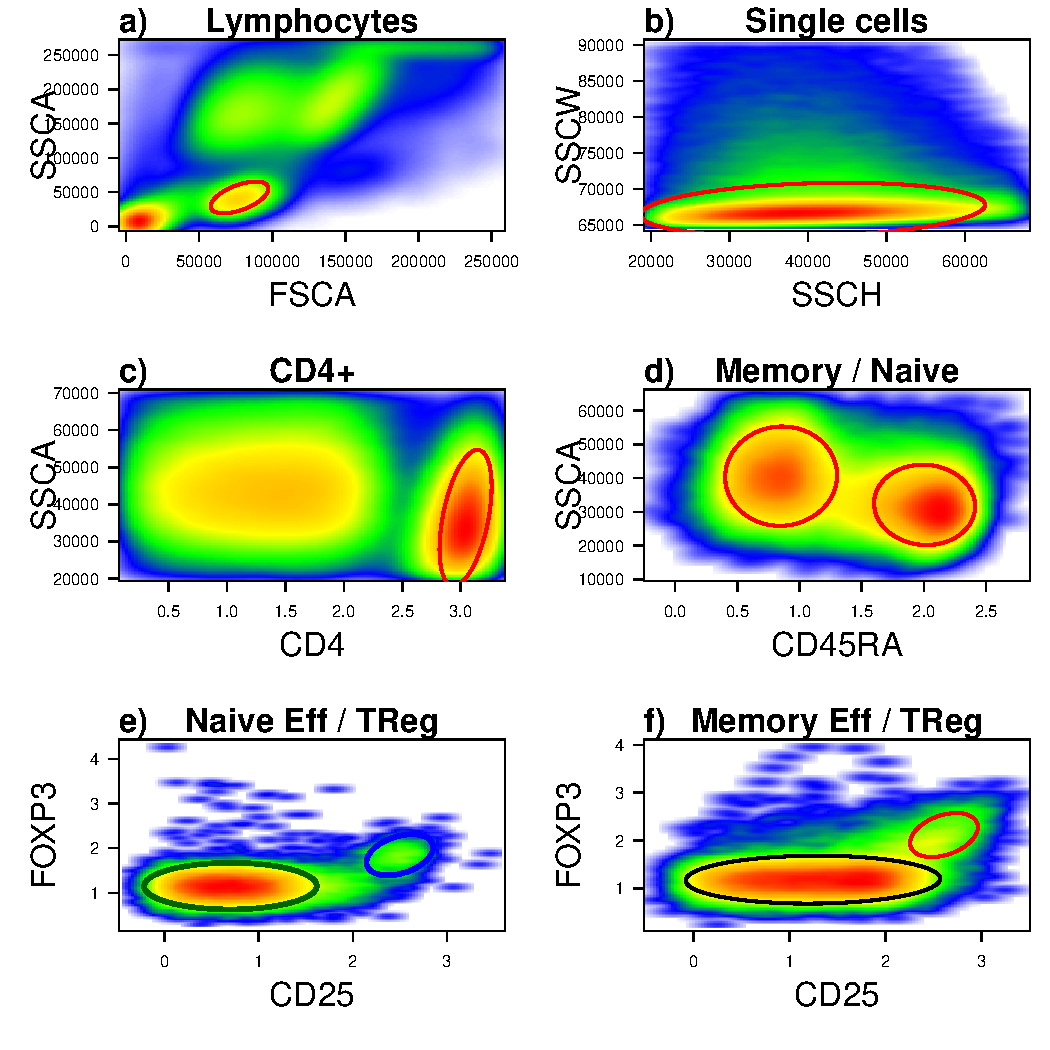
\includegraphics[scale=.75]{IL2/figures/CB00366X_2012-11-07.pdf}
%\caption{Resting sample.}
%\end{subfigure}
%\begin{subfigure}[b]{.4\textwidth}
%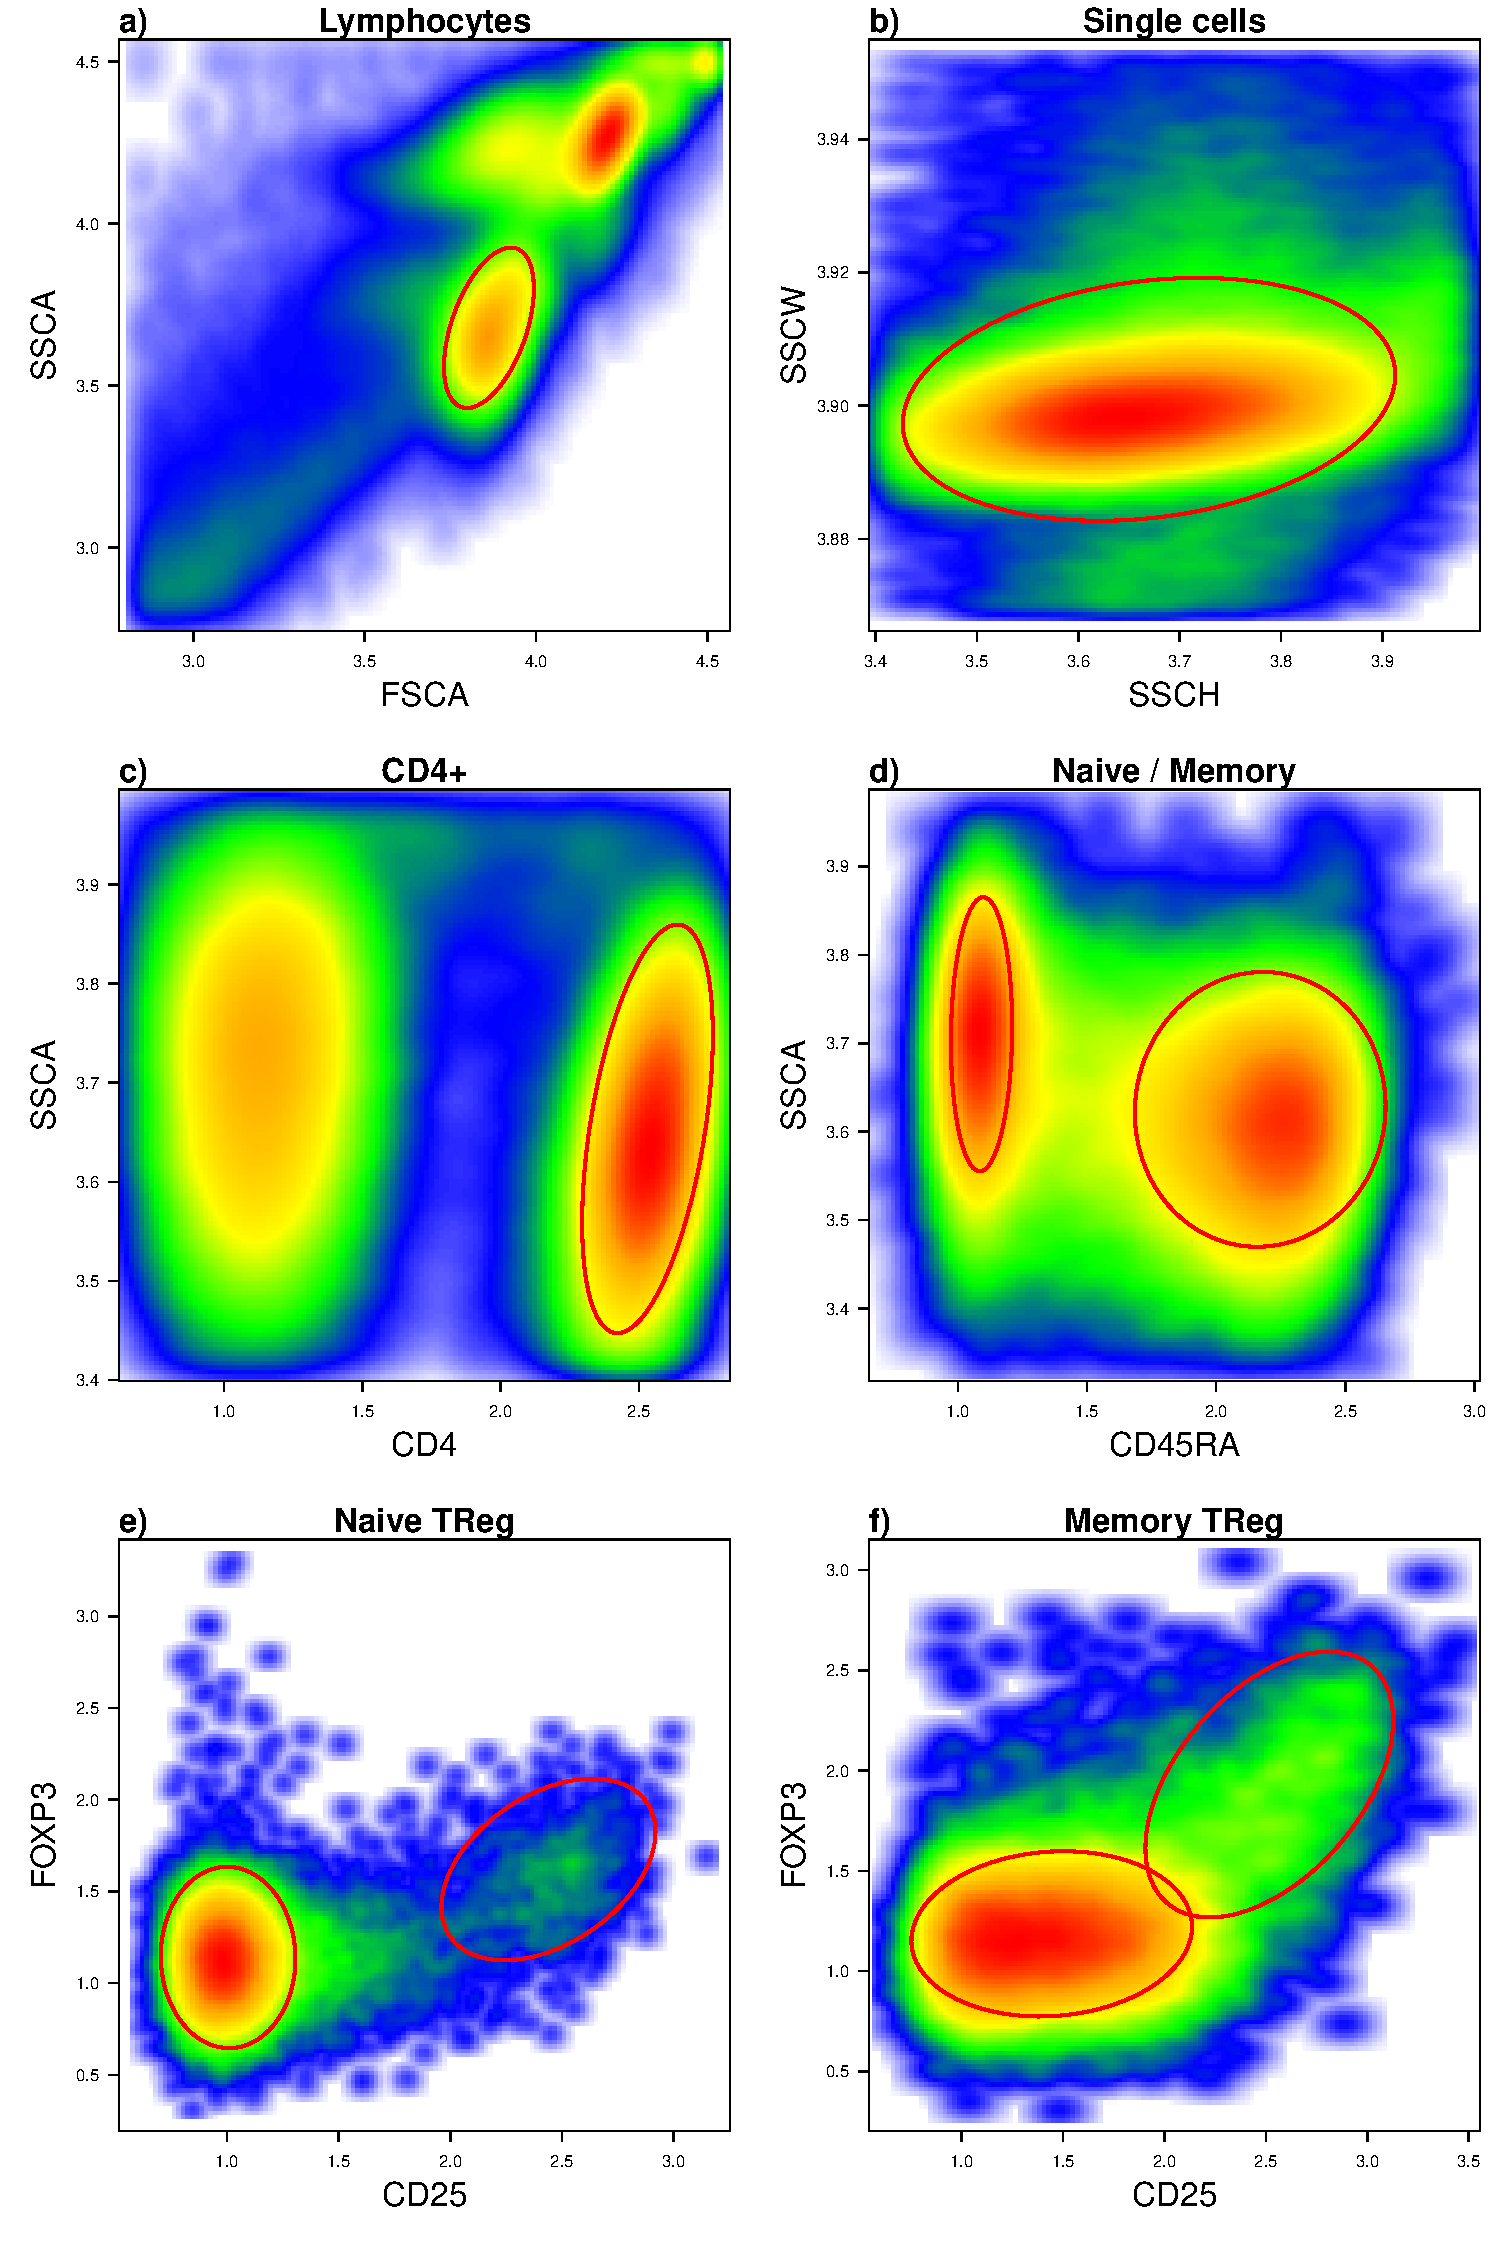
\includegraphics[scale=.25]{IL2/figures/manual-gating-CB00165D_01U_2012-11-29.pdf}
%\caption{Stimulated at 0.1 units of proleukin.}
%\end{subfigure}
%\begin{subfigure}[b]{.4\textwidth}
%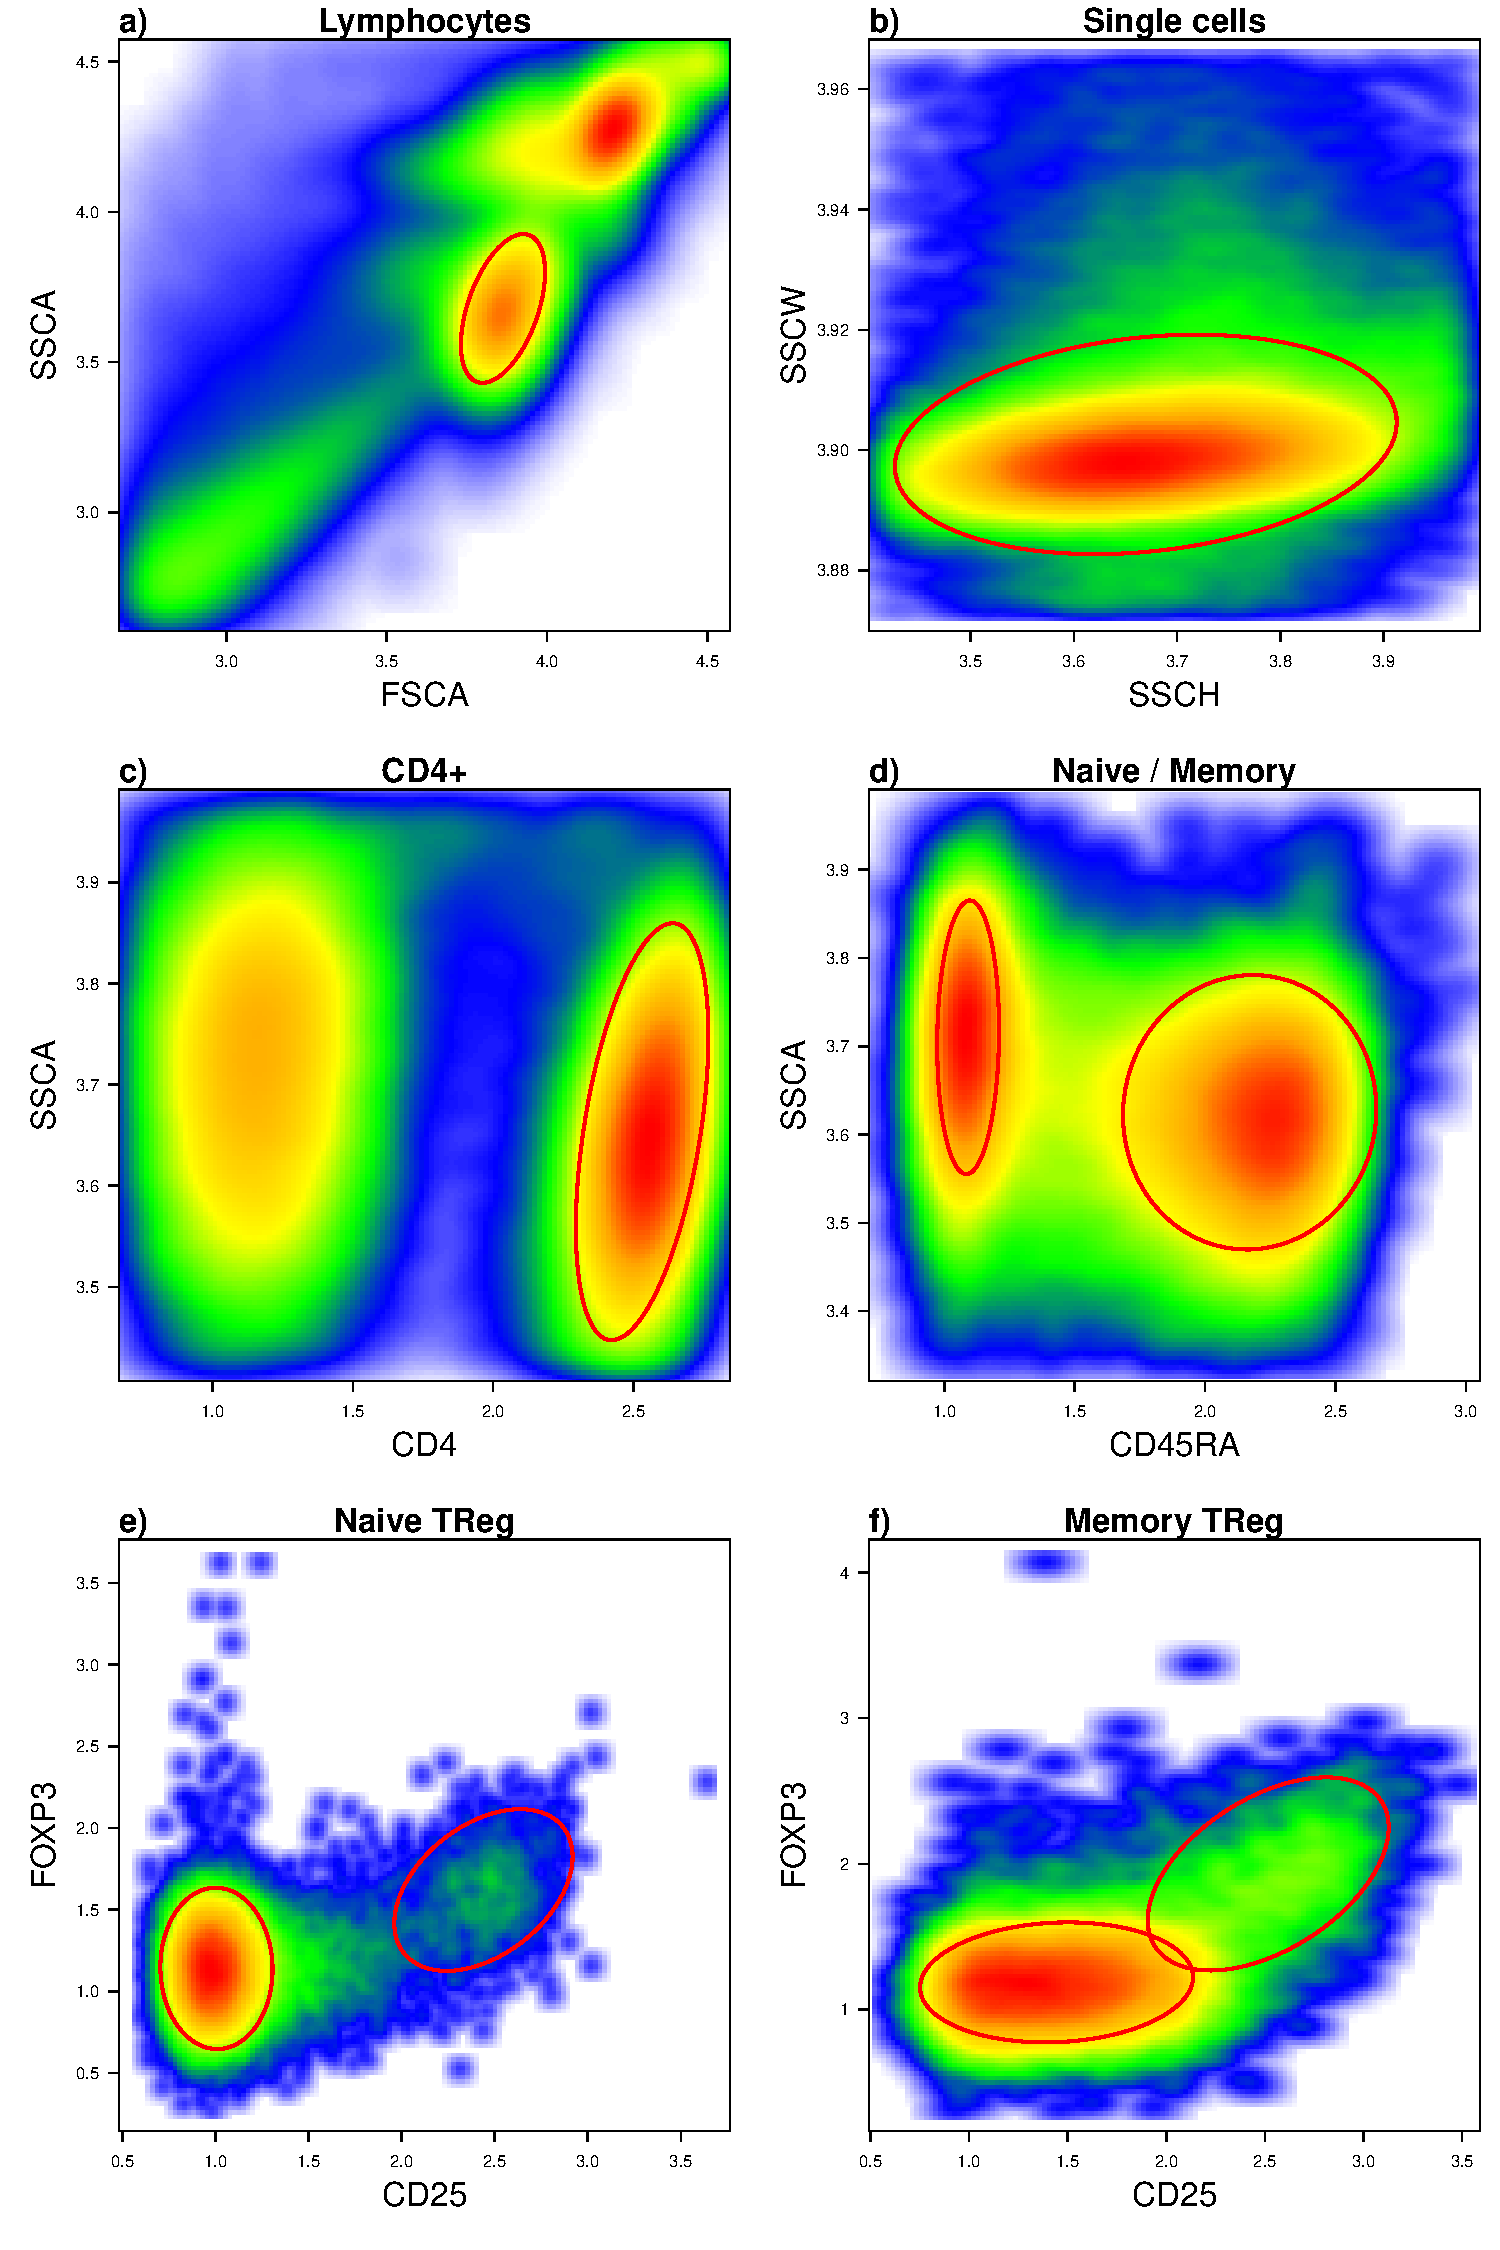
\includegraphics[scale=.25]{IL2/figures/manual-gating-CB00165D_10U_2012-11-29.pdf}
%\caption{Stimulated at 10 units of proleukin.}
%\end{subfigure}
%\begin{subfigure}[b]{.4\textwidth}
%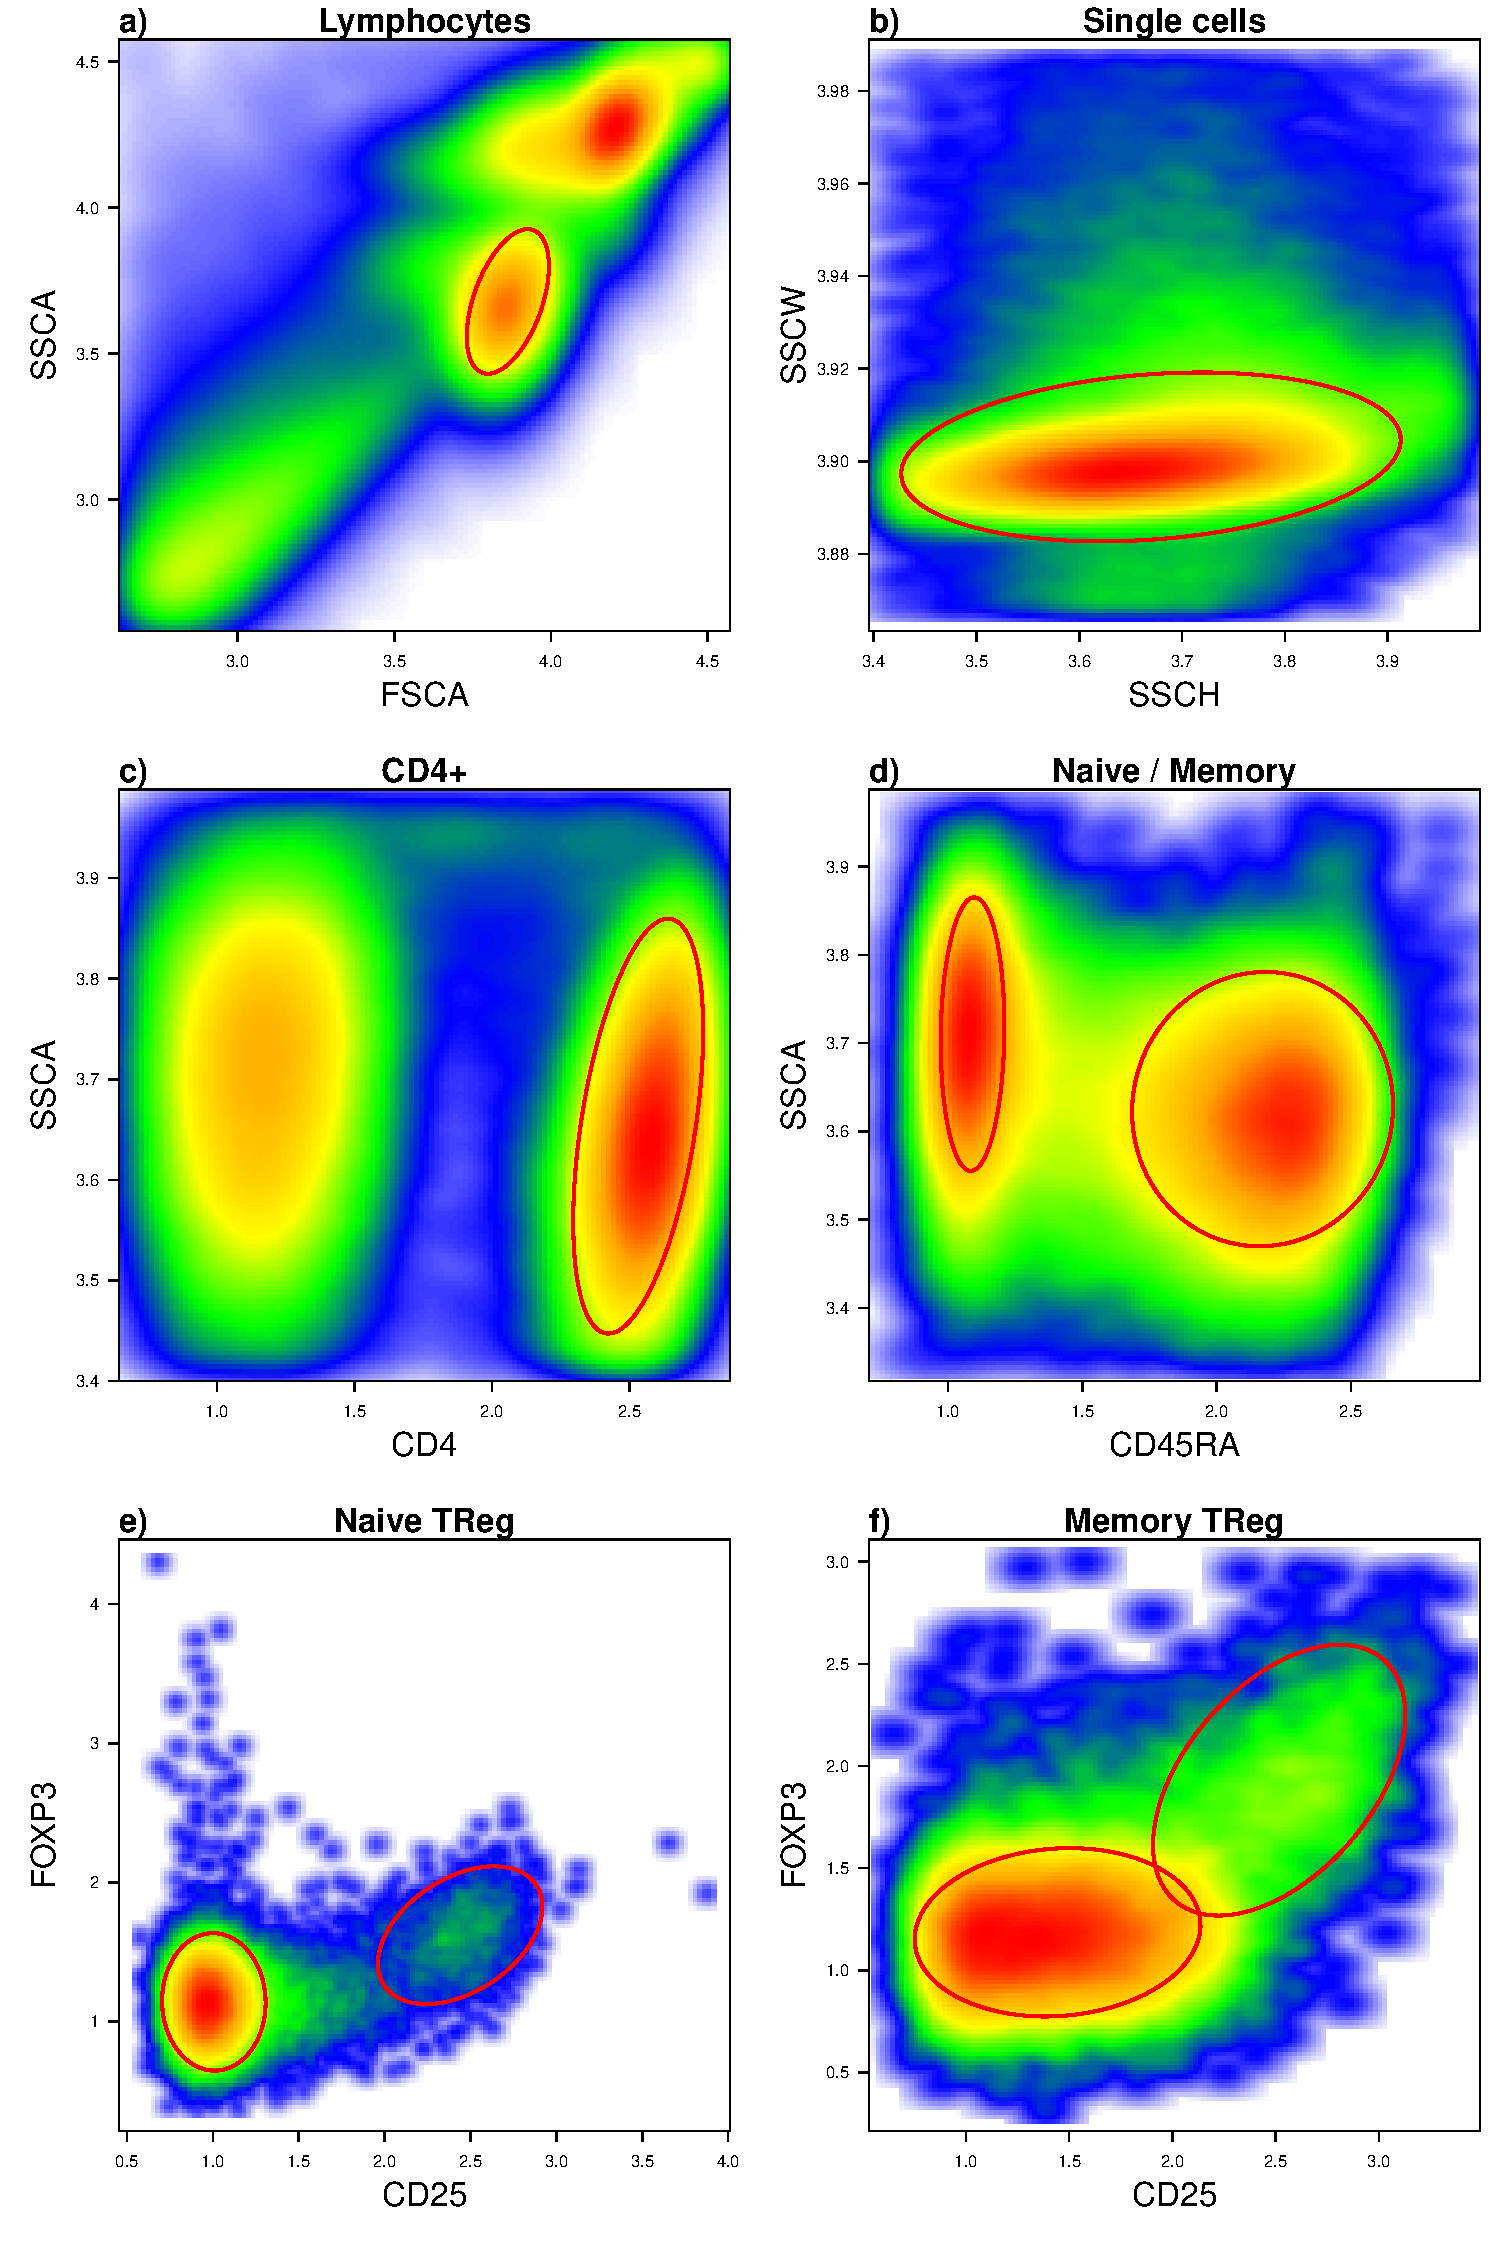
\includegraphics[scale=.25]{IL2/figures/manual-gating-CB00165D_1000U_2012-11-29.pdf}
%\caption{Stimulated at 1000 units of proleukin.}
%\end{subfigure}
\mycaption{figure:tony-cd4-gating}
{Gates applied across doses.}
{
Manual gating conducted using FlowJo by \contributor{Tony Cutler} to identify
naive effector and regulatory T cells (e)
and memory effector and regulatory T cells (f).
%The same gates can be applied across doses (i, ii, ,iii, iv).
}
\end{figure}


\hspace{-2cm}
\begin{figure}[h]
\centering
%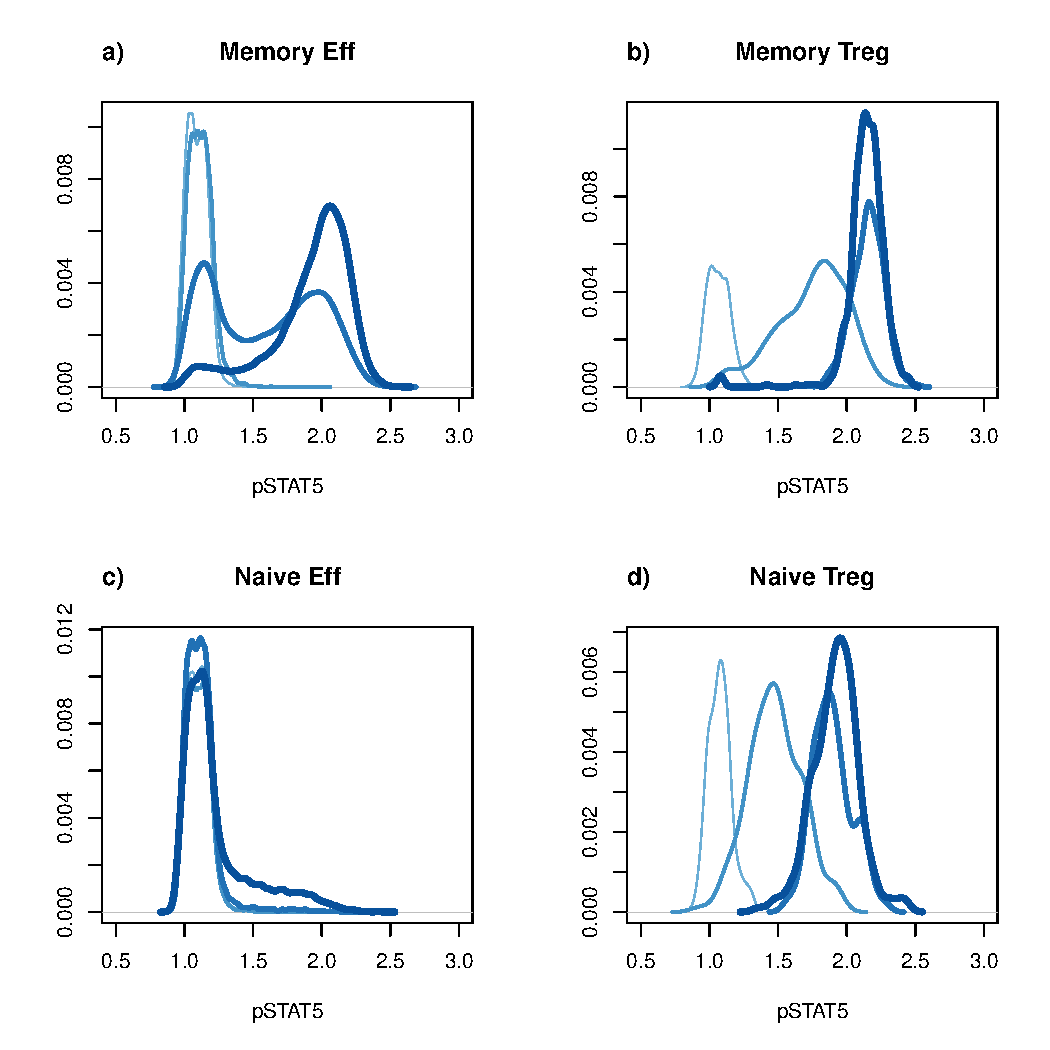
\includegraphics[scale=.45]{IL2/figures/dose-effect-pstat5-cellsubsets-density.pdf}
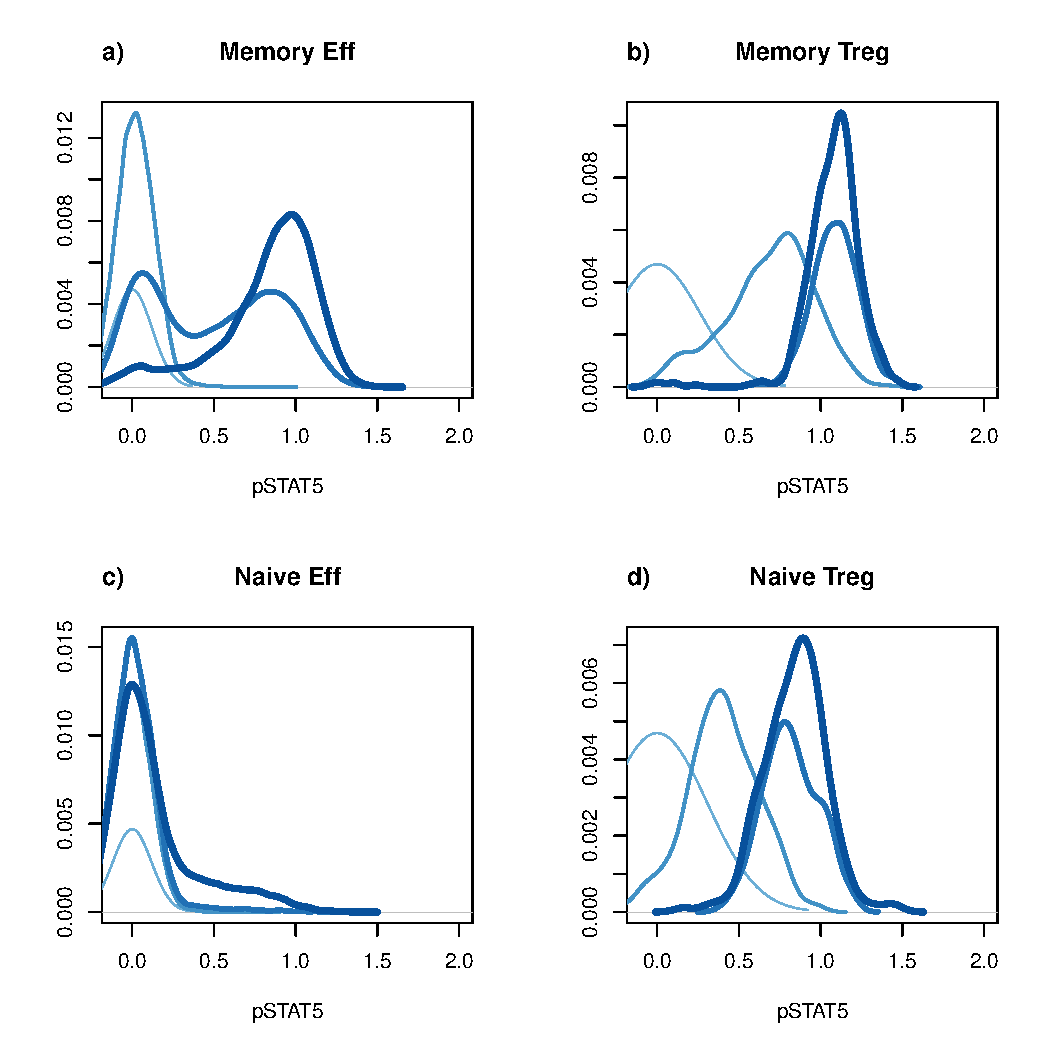
\includegraphics[scale=.45]{IL2/figures/dose-effect-pstat5-cellsubsets-density-baseline.pdf}
%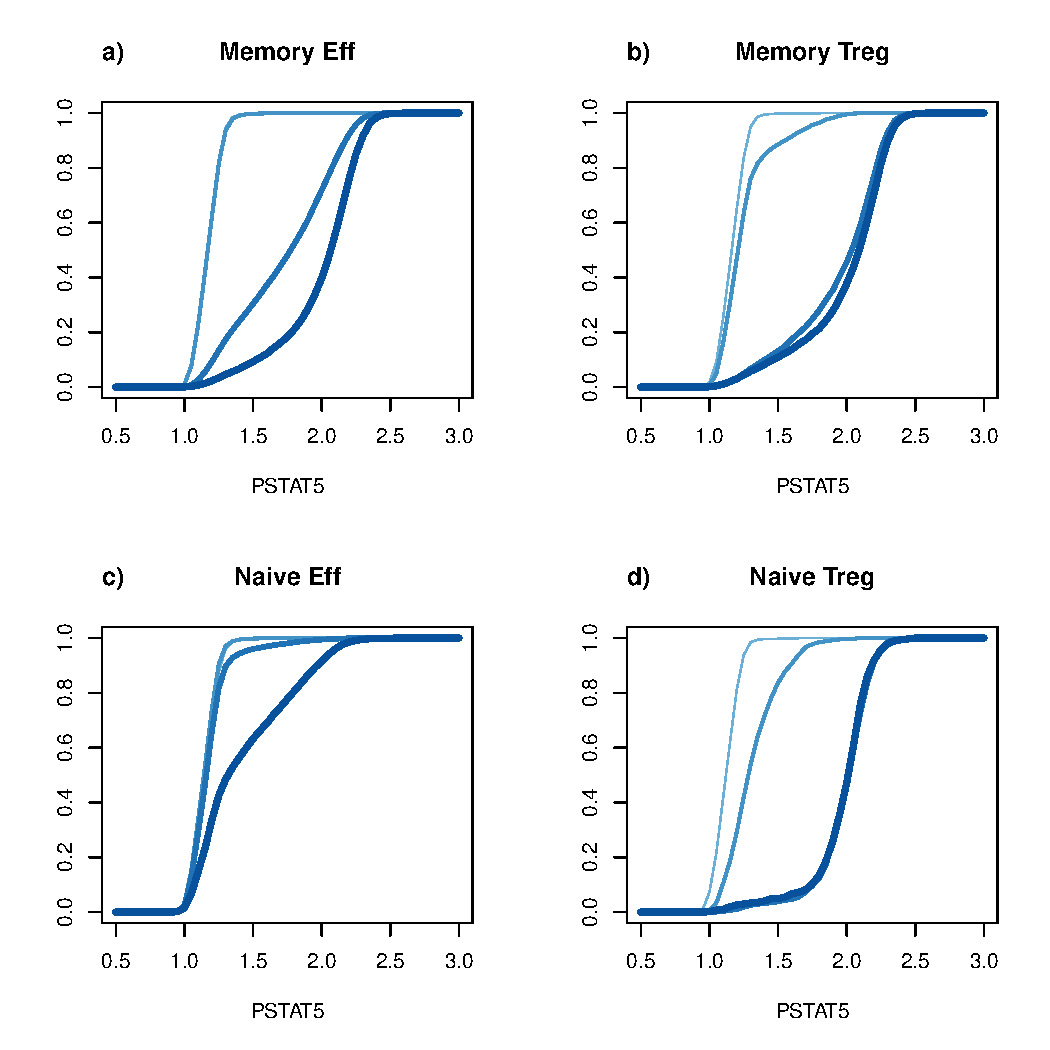
\includegraphics[scale=.45]{figures/dose-effect-pstat5-cellsubsets-ecdf-joined.pdf}
\mycaption{figure:dose-effect-pstat5-cellsubsets}
{ Distribution pSTAT5 in the manually gated cell subsets from \Cref{figure:tony-cd4-gating}. }
{
The thickness of the lines is representative of the four increasing doses of proleukin (0, 0.1, 10 and 1000 units).
The dose-response is most striking in the smaller subsets with high CD25 (b and d).
}
\end{figure}

%
%\hspace{-2cm}
%\begin{figure}[h]
%\centering
%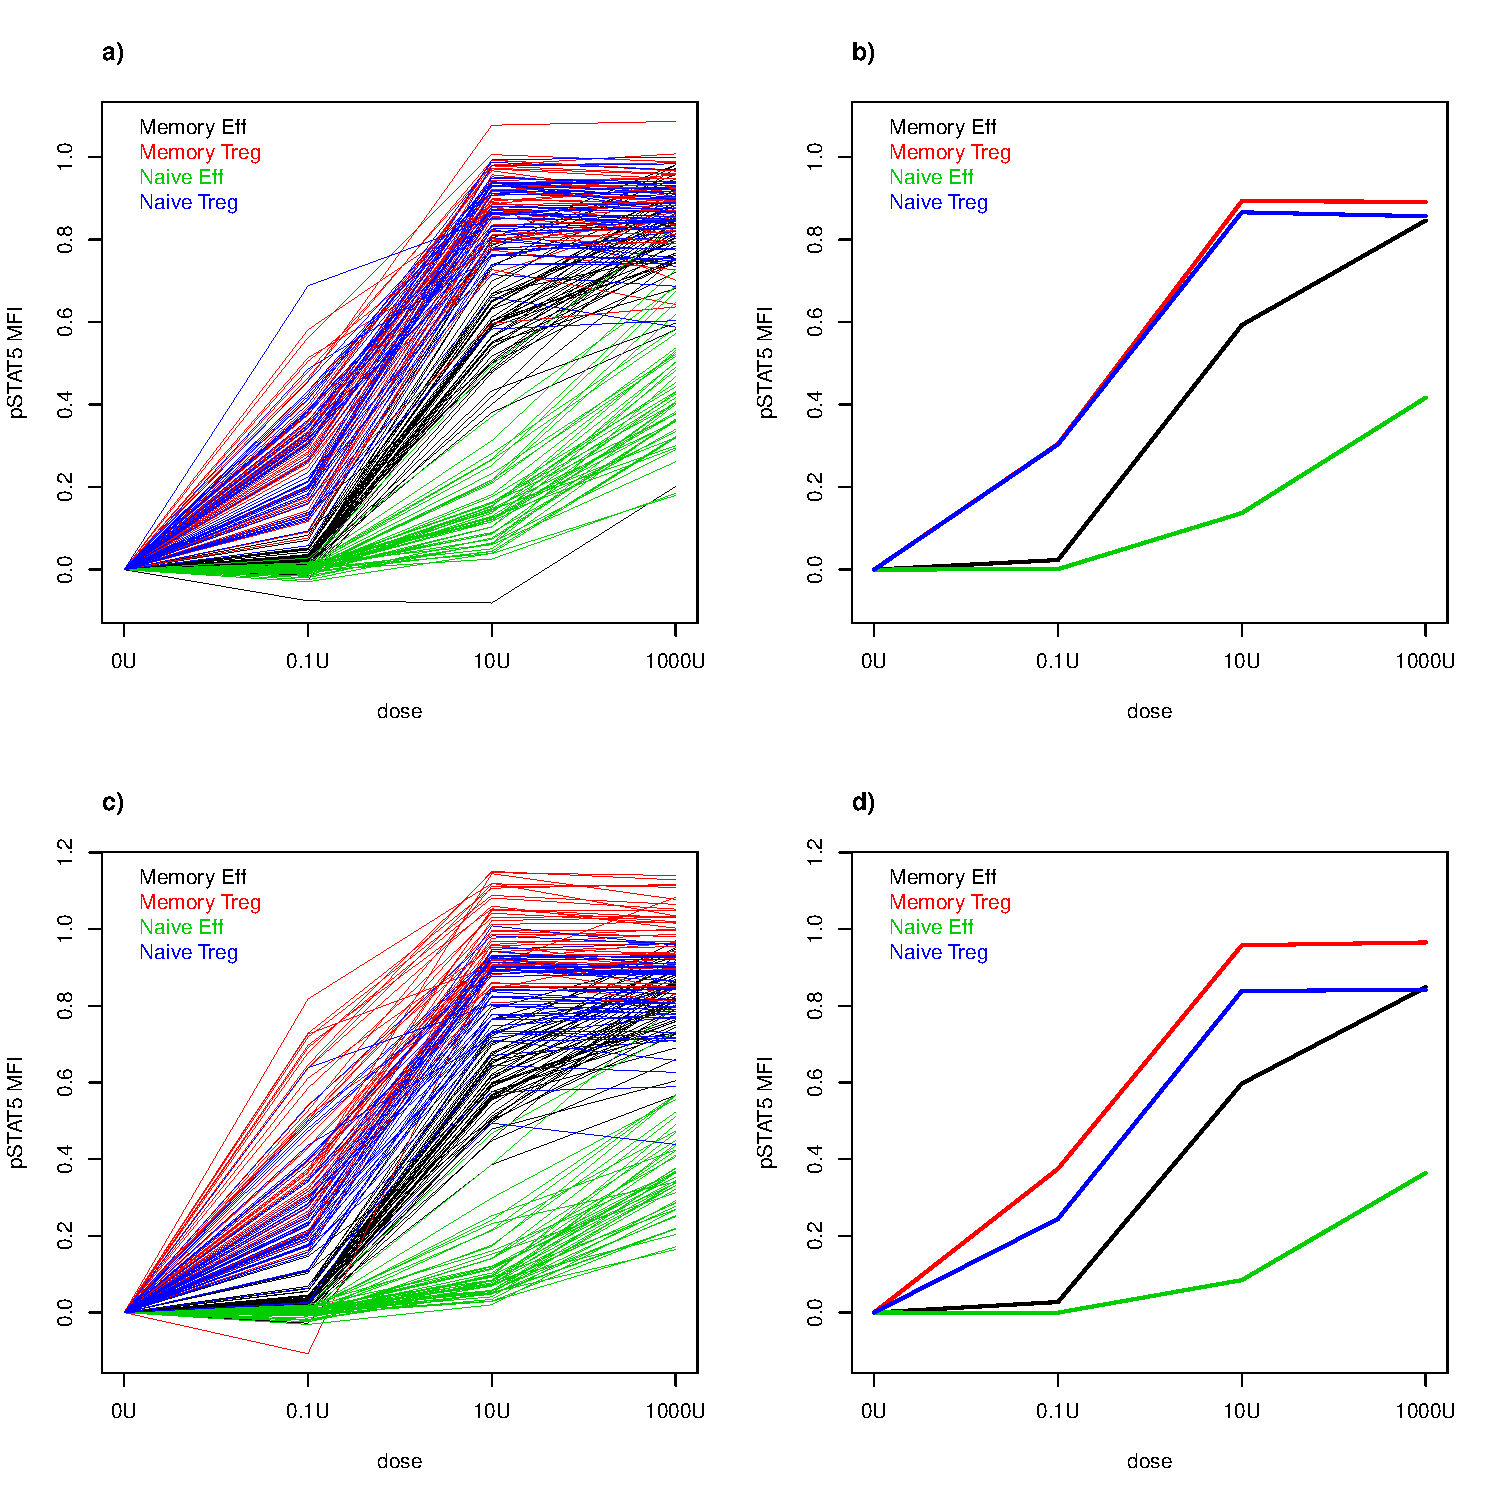
\includegraphics[scale=.4]{IL2/figures/pstat5-response-cellsubsets-manualgates.pdf}
%\caption{ \label{figure:pstat5-response-cellsubsets-gate}
%Fixed gates (a and b), magnetic gates (c and d).
%The response is measured in terms of baseline relative pSTAT5 MFI.
%a) The dose-response per cell-type in each sample obtained from manual gating with fixed gates.
%Note the outstanding memory effector sample is due to poor gating of the memory populatin in that particular sample.
%%CB01500E
%This in part due to the gate position but also because that sample does not have a clear memory population.
%b) The median dose-response per cell-type obtained from manual gating with fixed gates.
%}
%\end{figure}
%



\subsection{Reproducibility of pSTAT5 response within an individual}

Before proceeding with association testing of these cell phenotypes with T1D status or other covariates,
it is important to ascertain the repeatability of these cell phenotypes.
In order to test the repeatability, ten individuals where recalled for a second blood sample (\Cref{table:IL2-recalled-individuals}).
The repeatability of pSTAT5 MFI at all doses in each cell subset was tested using the manual gating and my method which allowed for
the gates to move so as to recenter on the data (\Cref{figure:repeatability-gating}).
It was found that overall the pSTAT5 MFI was poorly repeatable using both gating approaches,
with the most sensitive cells to proleukin, showing the worse repeatabilty in pSTAT5 MFI.
However, one issues is that pSTAT5 MFI is not very representative for very bimodal or skewed distributions such
as the memory effectors in \Cref{figure:dose-effect-pstat5-cellsubsets}.
Also the resting pSTAT5, which represents the baseline pSTAT5, of the same cell subset may not be constant across days.  
To address these issues, the percent of pSTAT5\positive cells was also assessed (\Cref{XXX}).
%To capture the response across all days, the sum of the pSTAT5 MFI was used.

Another method which captures the reponse of the whole distribution and not just the portion which crosses the positivity treshold,
is the area between the pSTAT5 CDF in the resting sample and the stimulated sample was used,
this relates to the Kolomogorov-Smirnoff distance which is defined as the maximum distance between the CDFs.

%The relative shift in the pSTAT5 distribution between resting and stimulated can be measured by computing the area between the cumulative density functions of the unstimulated and stimulated samples.
% As the pSTAT5 signal increases in a stimulated sample it is expected that the CDF shifts right.
% The resting provides the baseline.
%The area between the pSTAT5 CDF in the resting sample and the pSTAT5 CDF in the stimulated sample is measure of the strength of the response.

The repeatability of these three metrics was tested but none were found to be repeatable neither in the gated subsets nor any of the larger subsets (\Cref{XXX}).
Instead I decided to use the area under the pSTAT5 dose-response curve (\Cref{figure:pstat5-auc-celltypes}).

%Ten of these low responders from the Cambridge Bioresource were recalled for re-analysis to assess stability of this phenotype.
%However this cell phenotype was not found to be reproducible.  
%Using the automatically adjusted gates from manual gating, we assess the repeatability of the response in the four identified cell subsets.


%\hspace{-2cm}
%\begin{figure}[h]
%\centering
%%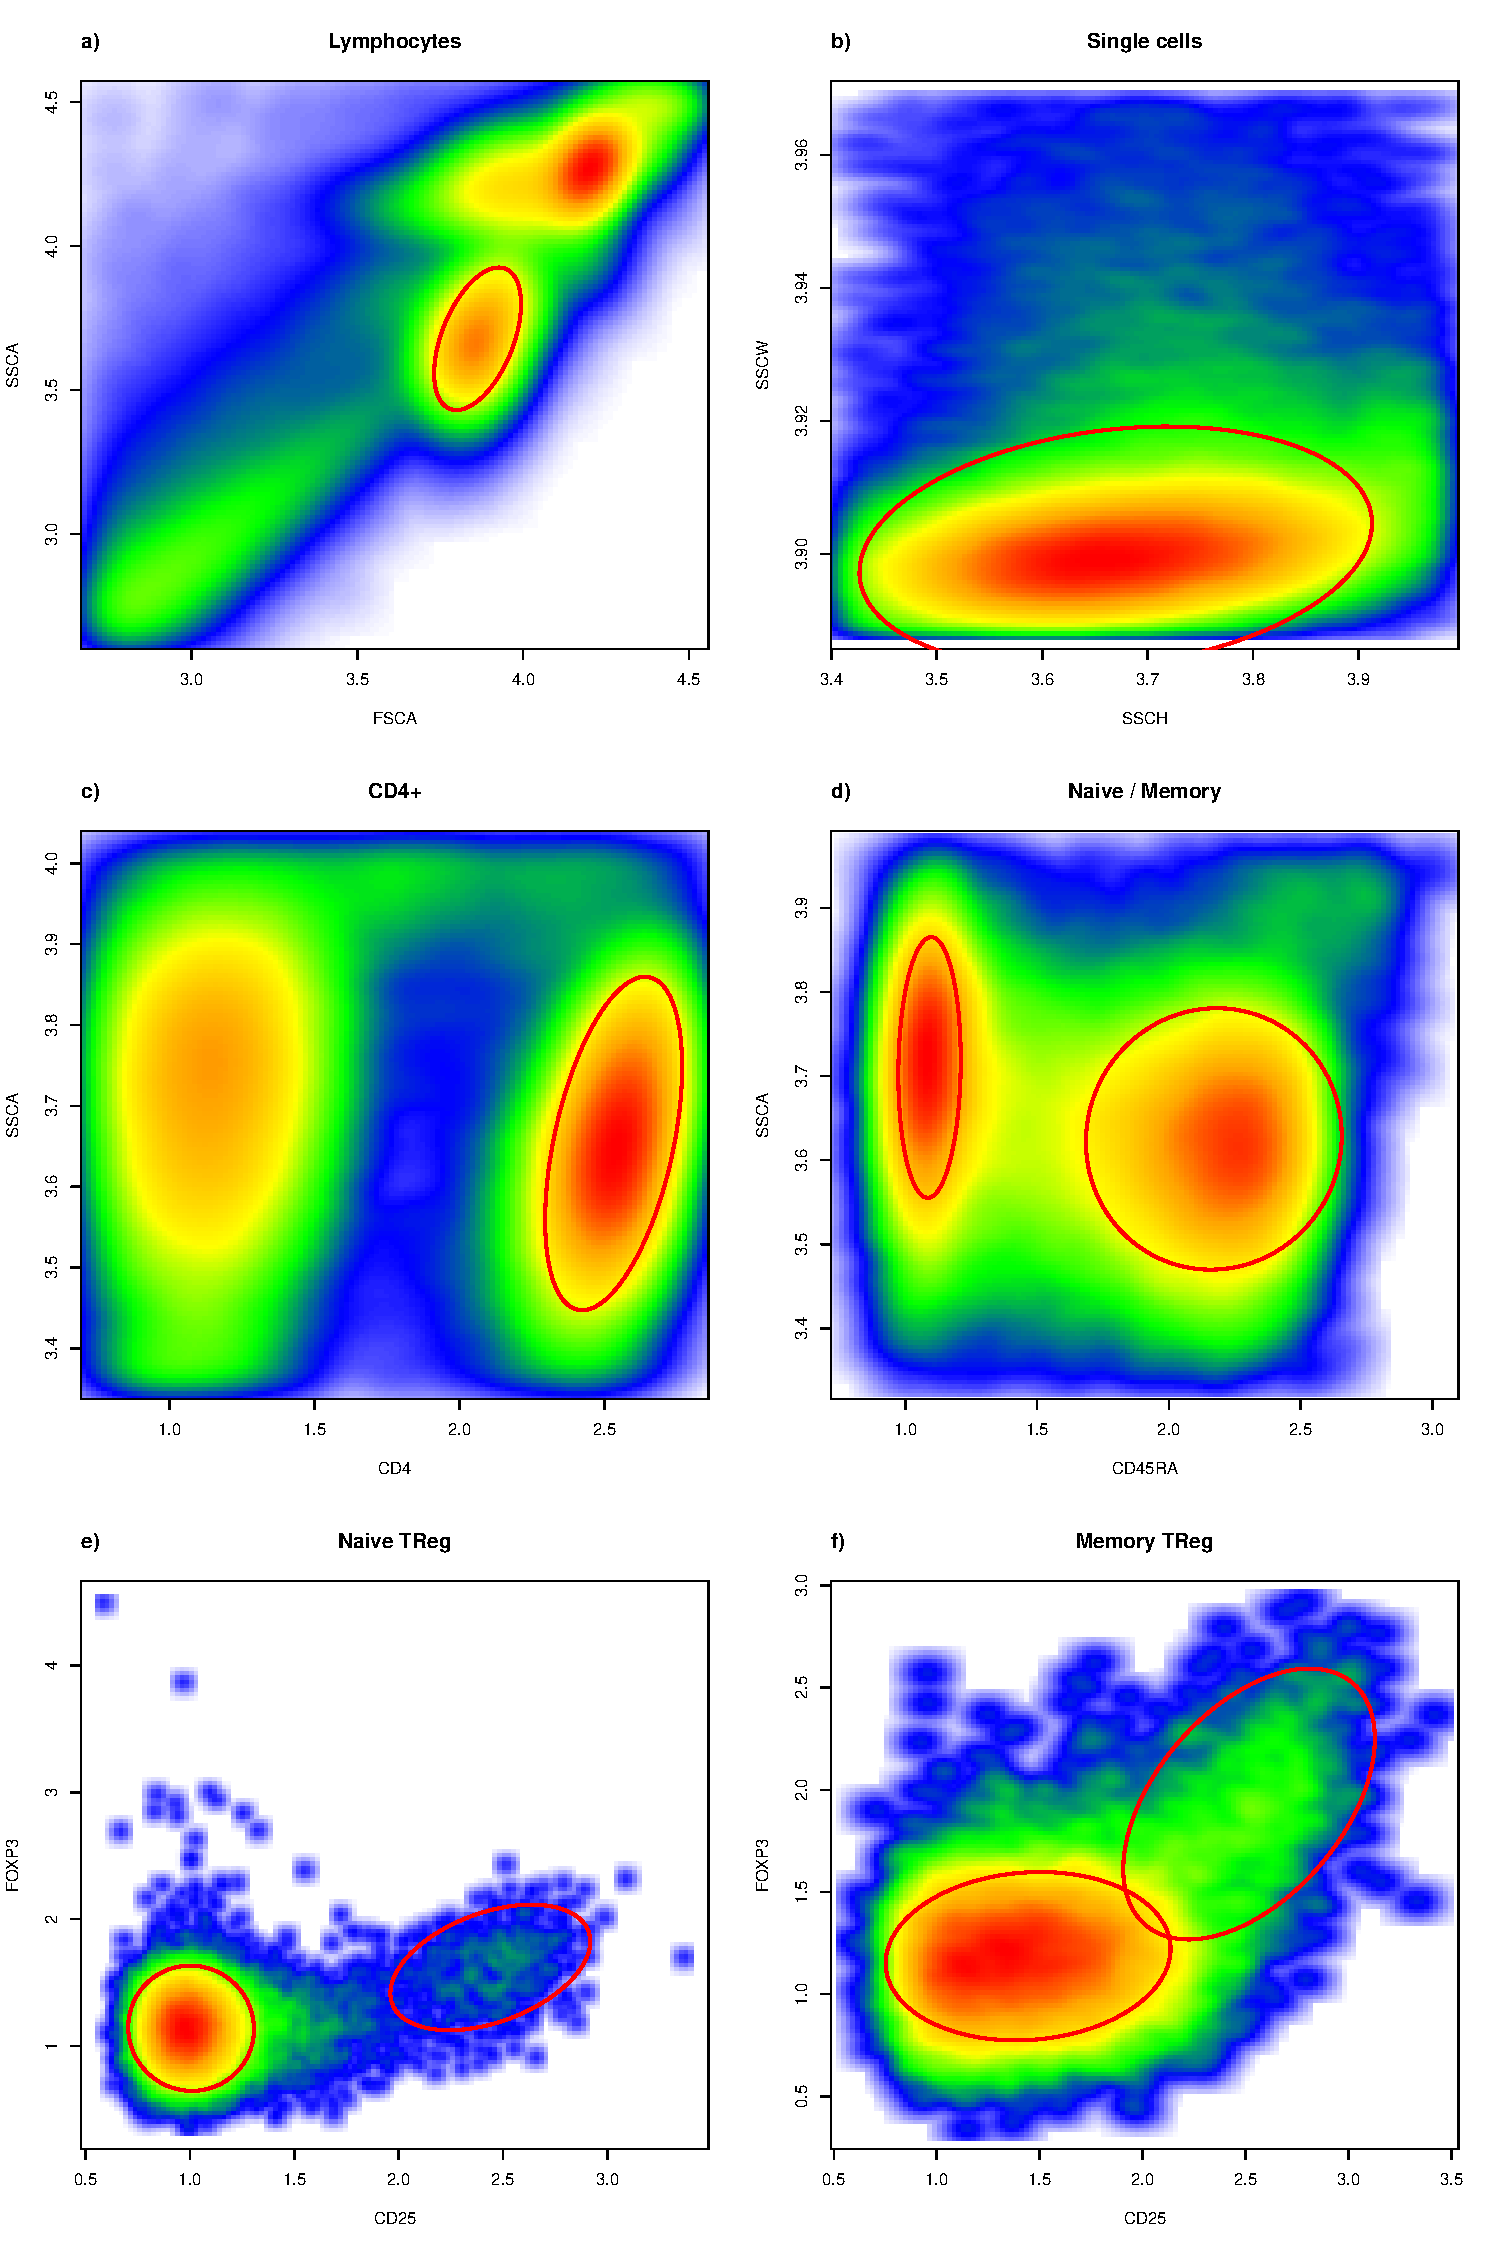
\includegraphics[scale=.5]{figures/manual-gating.pdf}
%\begin{subfigure}[b]{.4\textwidth}
  %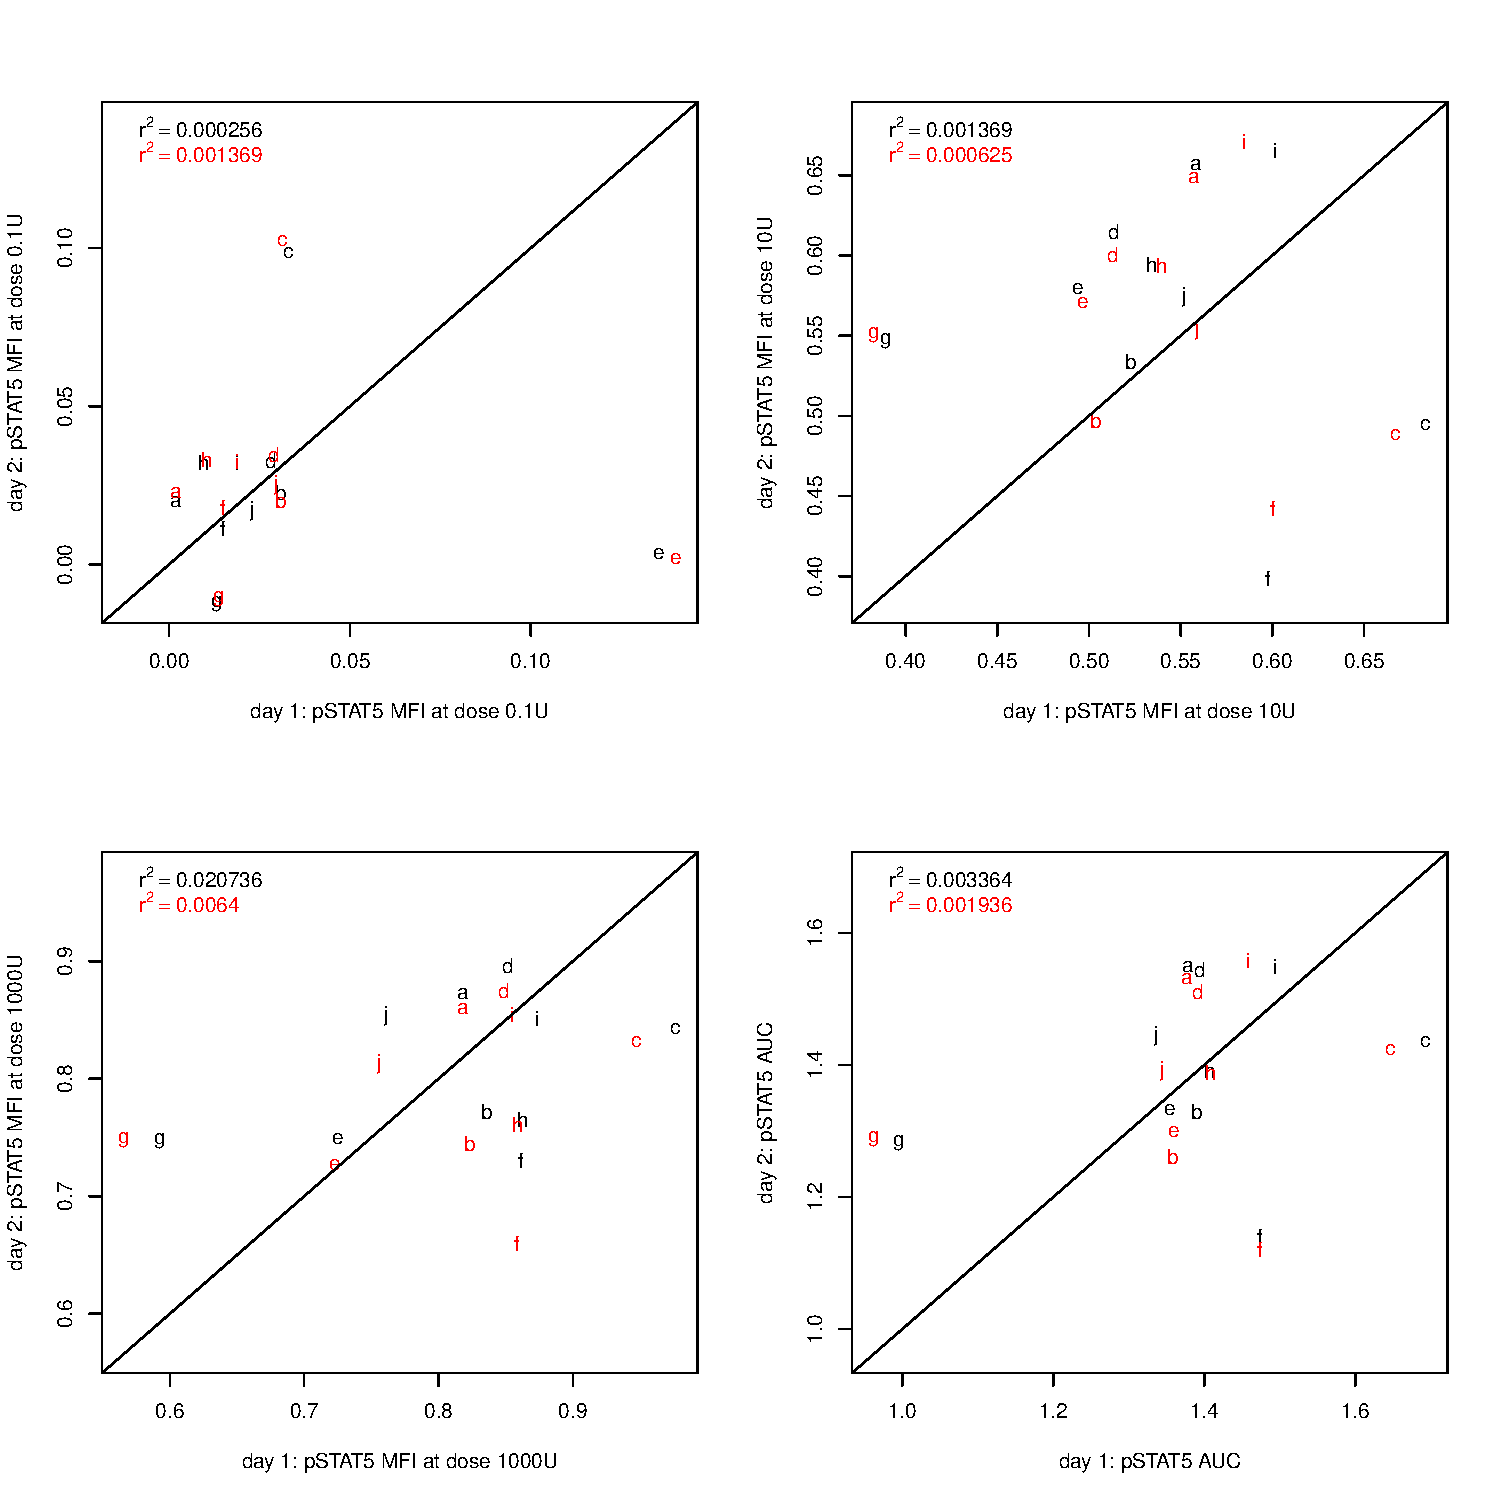
\includegraphics[scale=.25]{IL2/figures/repeatability-pstat5-mfi-Memory-Eff.pdf}
%\caption{Memory Effector}
%\end{subfigure}
%\begin{subfigure}[b]{.4\textwidth}
  %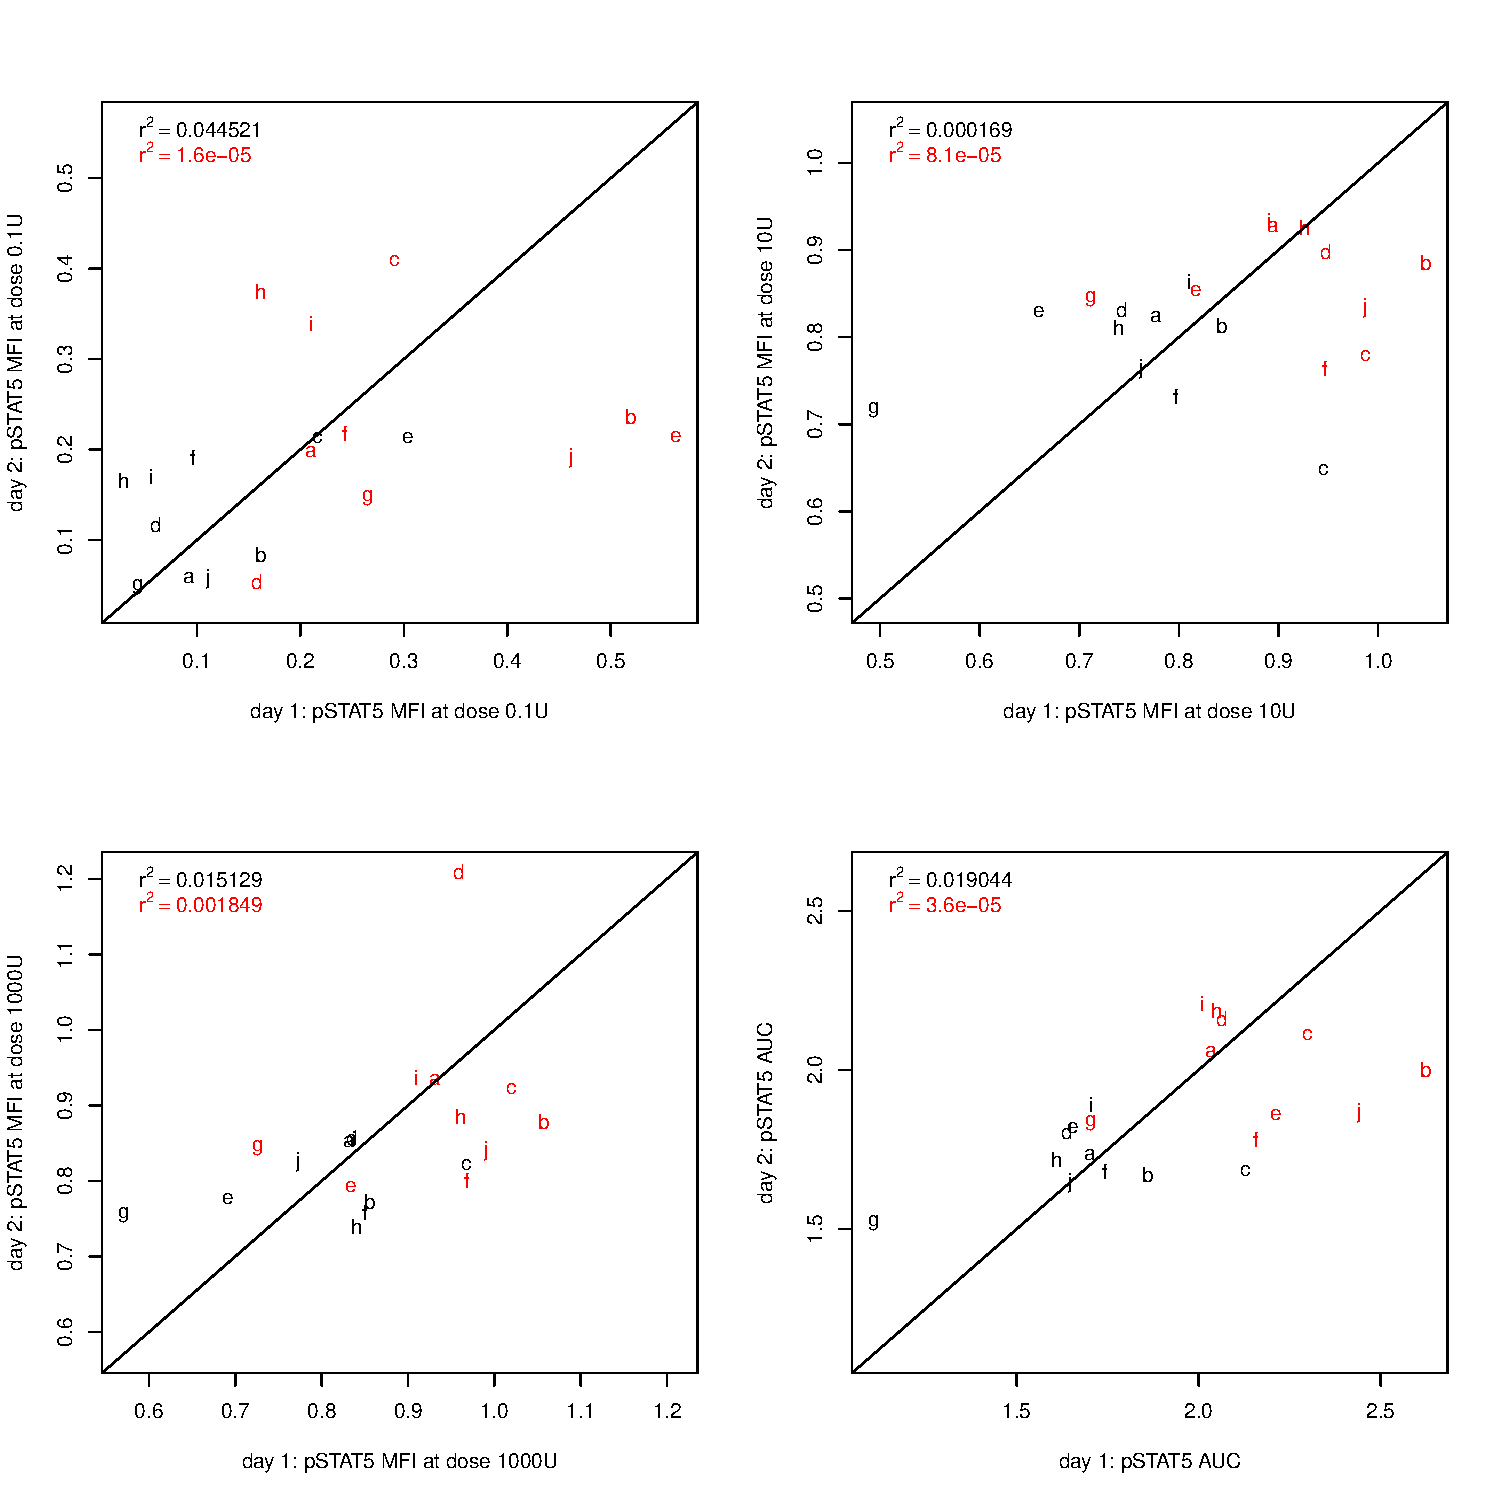
\includegraphics[scale=.25]{IL2/figures/repeatability-pstat5-mfi-Memory-Treg.pdf}
%\caption{Memory Treg}
%\end{subfigure}
%\begin{subfigure}[b]{.4\textwidth}
  %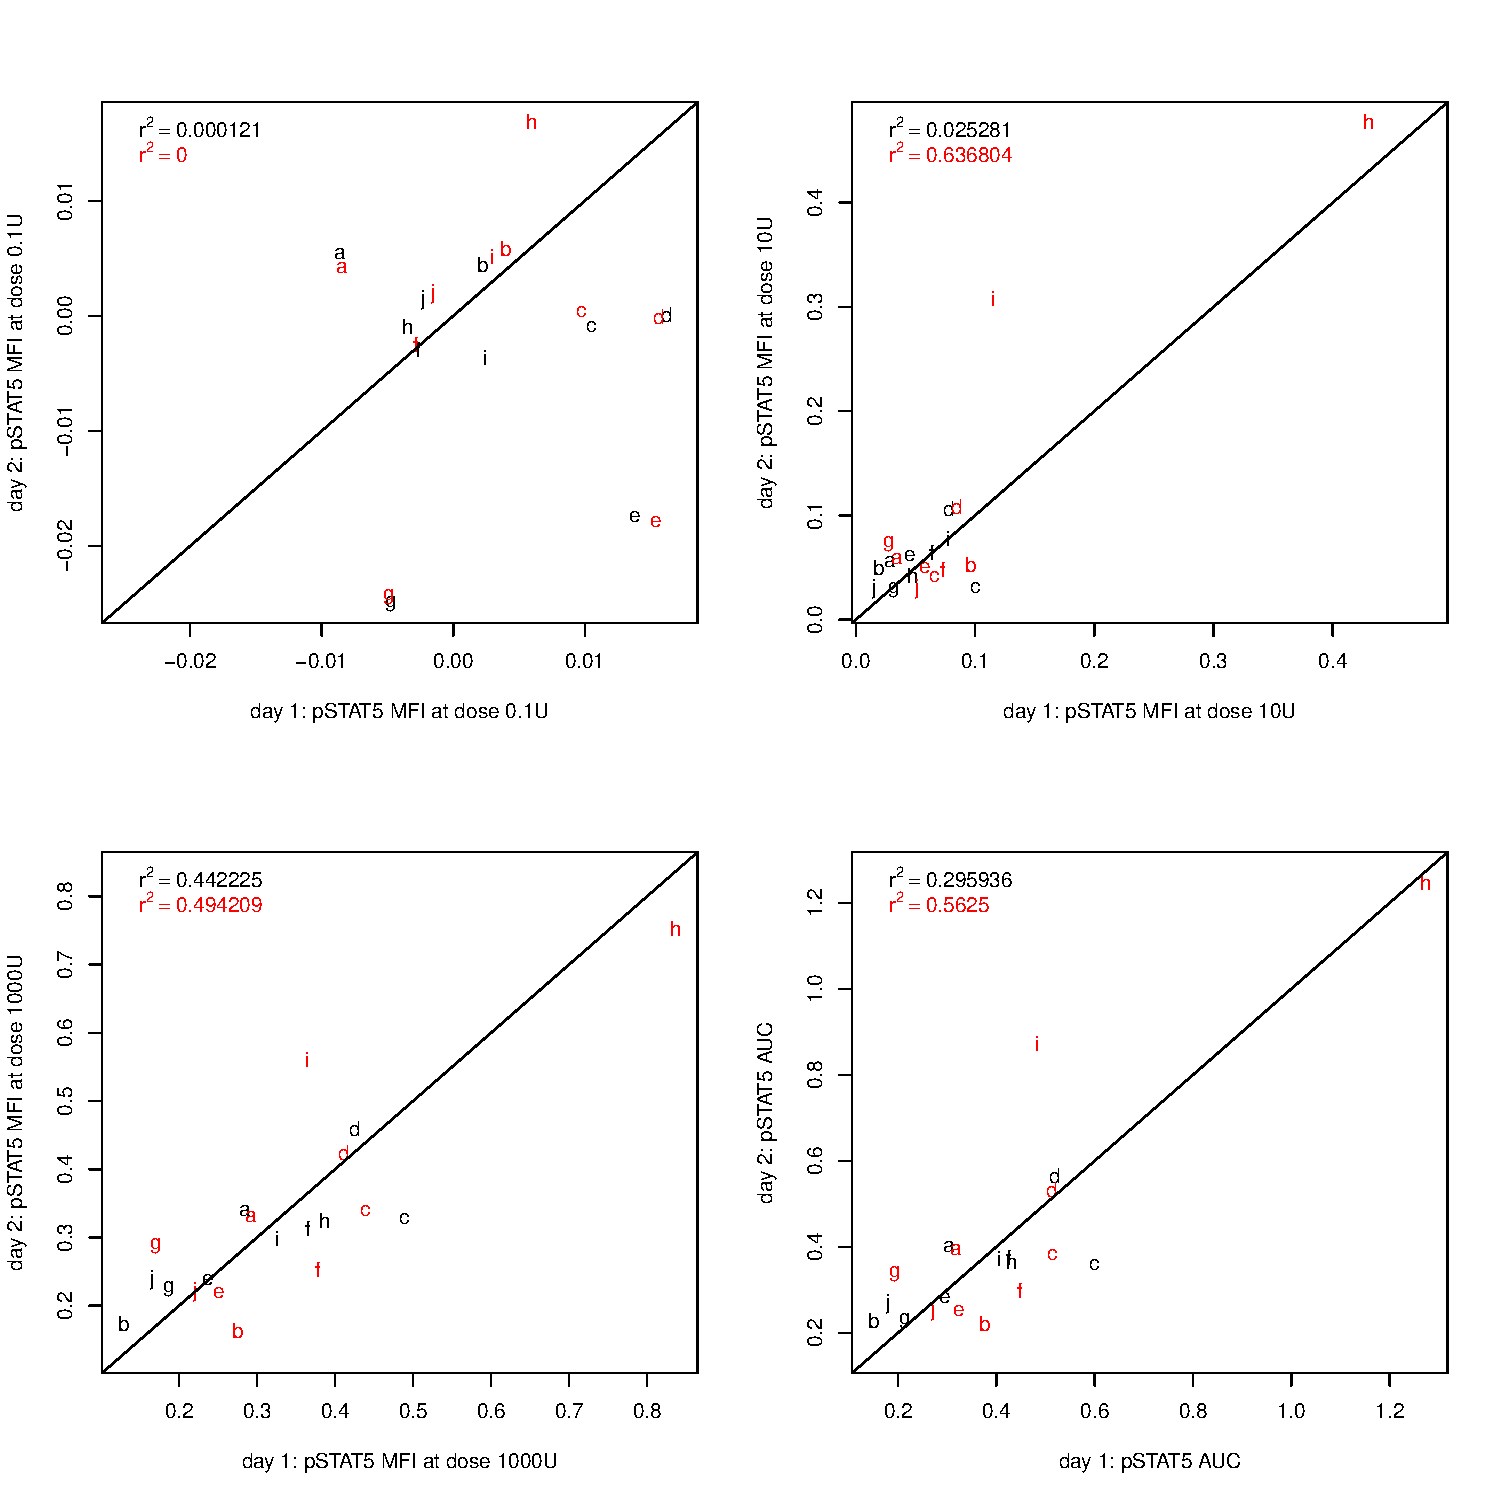
\includegraphics[scale=.25]{IL2/figures/repeatability-pstat5-mfi-Naive-Eff.pdf}
%\caption{Naive Effector}
%\end{subfigure}
%\begin{subfigure}[b]{.4\textwidth}
  %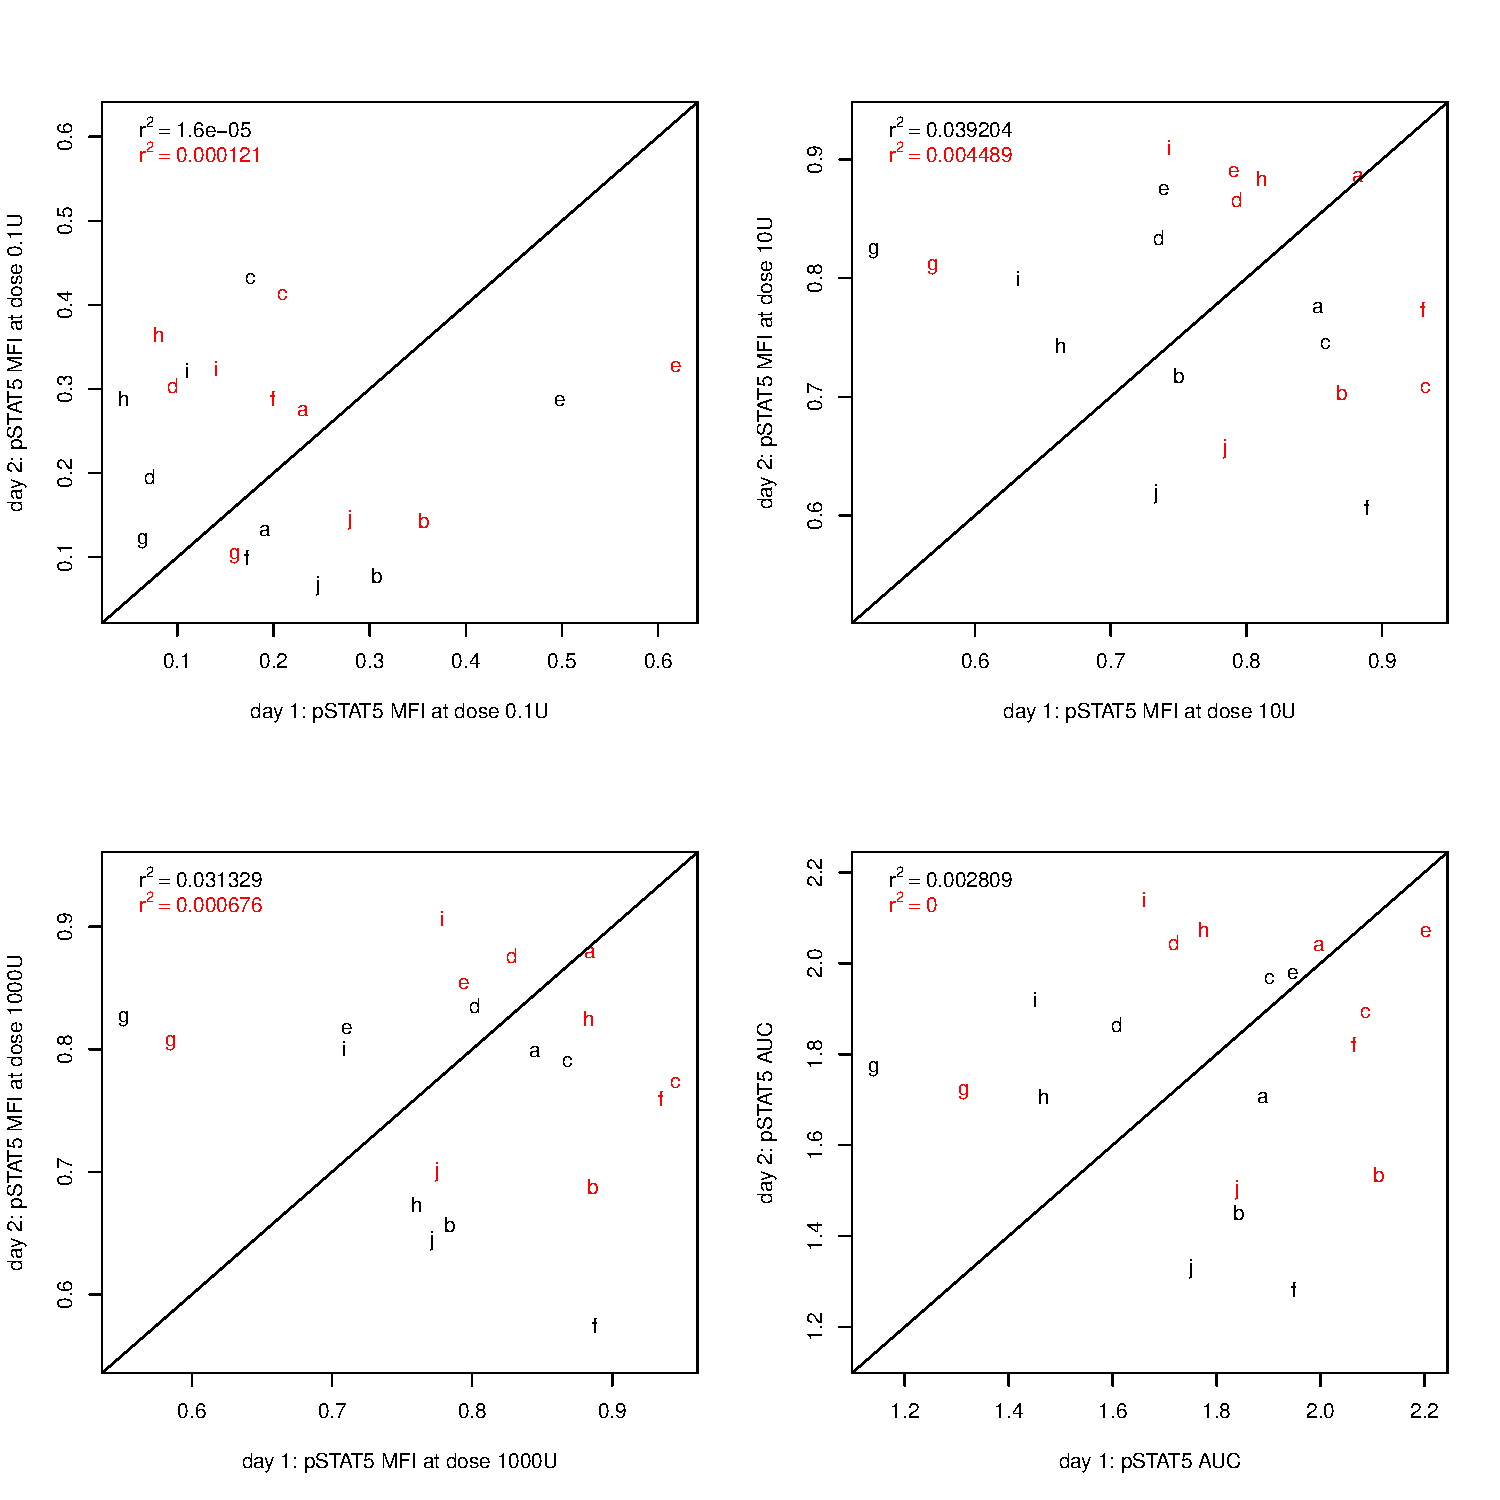
\includegraphics[scale=.25]{IL2/figures/repeatability-pstat5-mfi-Naive-Treg.pdf}
%\caption{Naive Treg}
%\end{subfigure}
%\caption{
%\label{figure:repeatability-gating}
%In black manual gates, in red magnetic gates.
%The AUC is the area under the dose response curve.
%}
%\end{figure}
%

\subsection{Normalisation of pSTAT5 improves repeatability}

%Normalisation can rely on peak alignment of the ungated sample but the peaks are often hard to reliably identify.
%The fluorescent marker required for pSTAT5 is Alexa Fluor 488
%Absolute MFI is a not a reliable way to assess pSTAT5.
%We need to subtract the background mfi.
%We can either do this on a cluster basis or use ann joining.
%What is more repeatable?  

%NO OPTIMAL TRANSFORM ACROSS ALL SAMPLES!!!
%Per sample transform required like flowClust but using the sliding window approach.
%Some prior knowledge is required to know what makes a sensible density plot.
%Care needs to be taken not to introduce spurious peaks.

Given the poor repeatability of pSTAT5, I was keen on seeking a normalisation technique that could improve the repeatability.
The approach of using beads on the same fluorochrome Alexa-488 used for pSTAT5 (\Cref{table:IL2-panels}),
as applied to CD25 normalisation in Chapter 2, 
%\Cref{chapter:il2ra}
did unfortunately not adequately capture the short term variation in pSTAT5 (\Cref{figure:pstat5-beads}).

\begin{figure}[h]
    \centering
    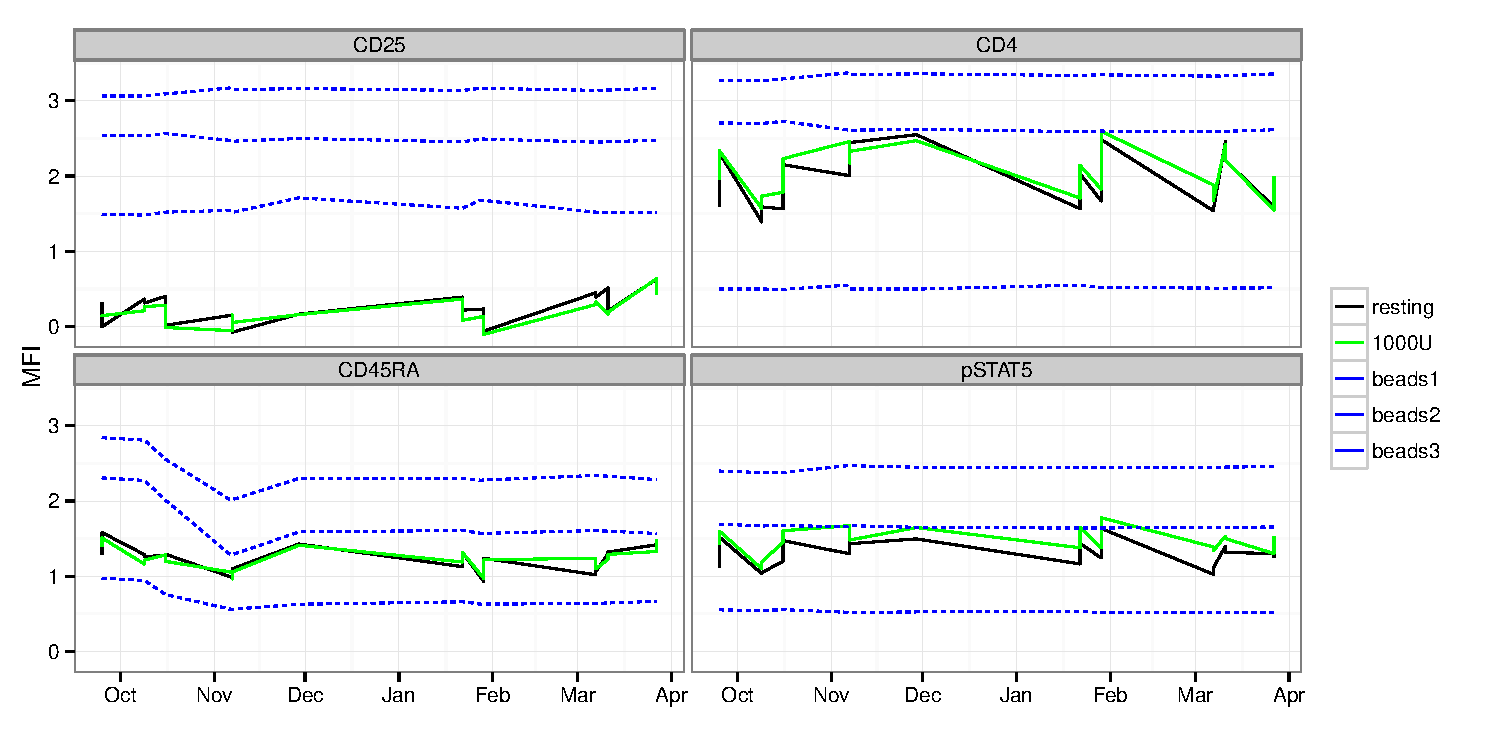
\includegraphics[scale=.5]{IL2/figures/beads.pdf}
    \mycaption{figure:pstat5-beads}
    {Variation in sample MFI is not captured by variation in bead MFI.}
    { }
\end{figure}

Instead, I applied another normalisation technique, akin to the method applied in Chapter 3 on qPCR data to align common copy number groups 1 and 2 across plates.
The method relies on the assumption that the the two peaks in the pSTAT5 distribution characteristic of stimulated and unstimulated cells,
should exist in all ungated samples, but their locations and their proportions may across doses and days.
%Given that the location of the peaks of pSTAT5 in the ungated sample remains fairly stable across doses but that the heights vary, this advocates a normalisation method which relies on peak alignment.
%If we expect that the core cell populations should exist in all samples but that their locations and their proportions may vary across days and \emph{IL-2} dose, a normalisation approach is to align the location of the population across doses per day.
Hence we wish to align the location of the peaks across days while allowing for the relative proportion of the populations to vary.  


The idea is to identify the groups based on a single marker by clustering algorithm and then selecting the peaks to be the group medians.
In this approach the number of groups K needs to be known a priori and is assumed to be the same across samples.
%This is the method used by \Rpackage{flowBeads} which identifies groups with the k-medoids algorithm for the purpose of bead normalisation.
%However peaks are not always easily identifiable.
In Chapter 3, I used k-means to identify the peaks, but I found on this data k-means and k-medoids performed poorly since the cluster variances are very different.
The second peak corresponding to the stimulated cells is much broader and smaller since the majority of cells in the sample are not stimulated.
A mixture model algorithm would be better suited since it allows for different variances in the clustering.
but because of the skewness of the data, the peaks did not correspond to the cluster medians.
Instead, I used a sliding window approach on the density function.
The sliding window approach records the point with the highest density estimate in the current window,
so that within a window of twice the span the point of highest density is selected as a peak.
A list of highest density points is returned of which the top K may be selected.
This is in fact one of the approaches implemented in the \Rpackage{flowStats}.
I found in practise this method to work well with a window size of $40$ across all samples considered.
%This approach is useful for estimating K but the window size may need to be tuned per sample.

Unfortunately in flow cytometry, the peaks are not always clearly identifiable due to the nature of the staining and the transform which can introduce
spurious peaks close to zero (\Cref{appendix:transformation,appendix:normalisation}).
The choice of the transform plays a crucial role, especially regarding points around zero since spurious peaks are introduced if the wrong width parameter is selected
for the logicle transform.
This is particularly noteable in ungated data where debris obfuscate the pSTAT5 signal and can introduce artefactual peaks,
leading to peak misidenfication.
However I found that upon gating on lymphocytes and CD4\positive lymphocytes, these spurious peaks disappear and both peaks were correctly identified 
\Cref{figure:pstat5-peak-normalisation}.
In the CD4\positive lymphocytes, in order to facilitate peak identification, I considered the pSTAT5 distribution at 10 units instead of 1000 units,
as the unstimulated/stimulated ratio is more even at an intermediate dose since at the highest dose most CD4\positive lymphocytes are stimulated.
%Here's an example of this method applied on simulated data where the number of peaks is known and easily identifiable (Figure~\ref{figure:simulation-peak-align}).
%The sliding window method is good for detecting local maximums while the clustering approach is better at find global splits.
%Hence we combine both approaches by using the sliding window on the partitions identified by the clustering.
%We apply mclust and pam (clara) because mclust tends to the fit the data better when the cluster are of very uneven size like example (~/pam.fail.RDAta).
Once the two peaks have been identified in all samples, the next task is now to align for the purpose of normalisation.
A non-linear transform could be considered so that peaks may be aligned independently, but since there are only two peaks,
a linear transform is sufficient to perfectly map the peaks across all samples \Cref{figure:pstat5-peak-normalisation}.
After appliying this transform to the previously gated pSTAT5 MFI and retested the repeatability.

%We also apply this method the pSTAT5 positivity threshold
%how?


\begin{figure}[h]
    \centering
    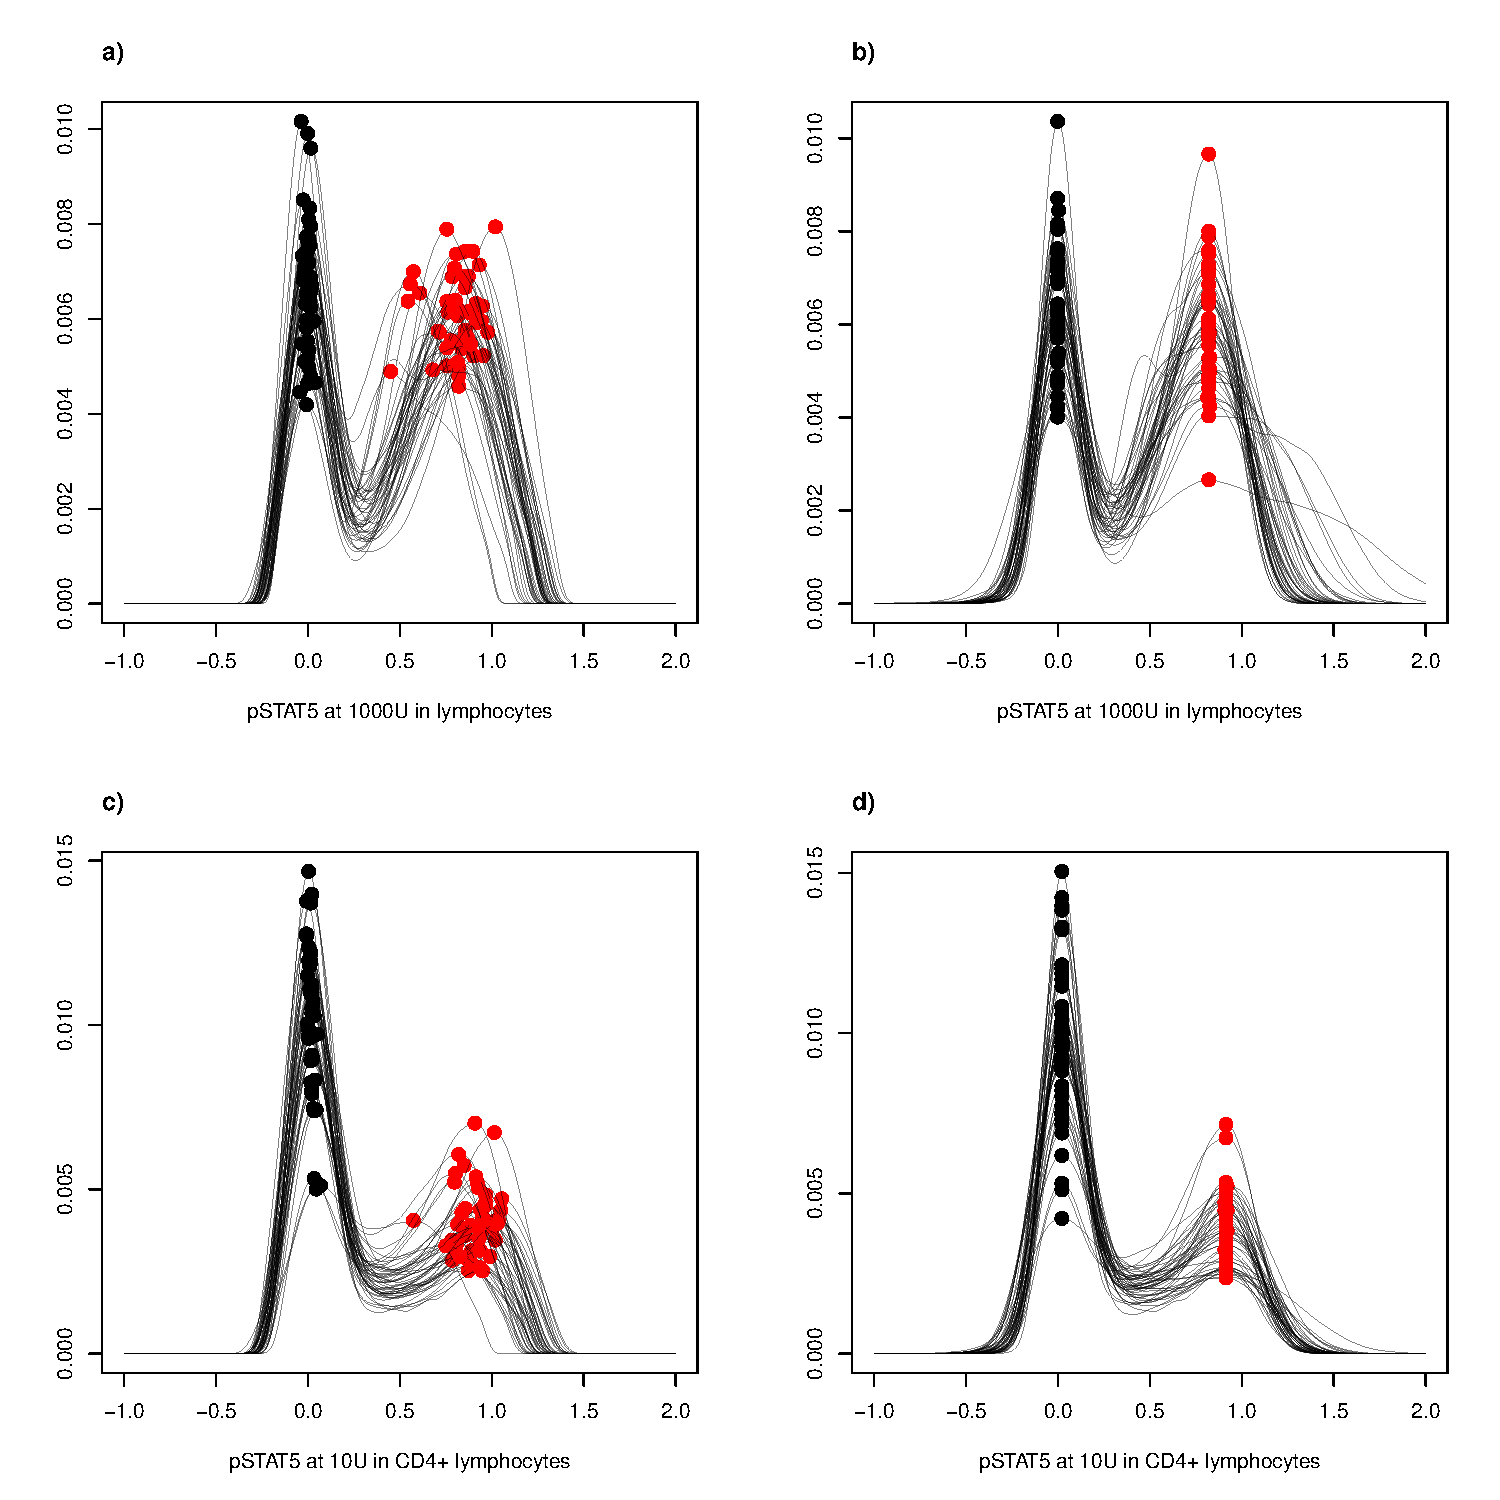
\includegraphics[scale=.5]{IL2/figures/pstat5-peak-normalisation.pdf}
    \mycaption{figure:pstat5-peak-normalisation}
    {Normalisation by peak alignment of the pSTAT5 distribution in lymphocytes (a and b) and CD4\positive lymphocytes (c and d).}
    {
      The two peaks of the pSTAT5 distribution are identified using a clustering/sliding window approach,
      in the lymphocyte sample stimulated at 1000 units (a) and in the manually gated CD4\positive lymphocyte subset stimulated at 10 units (c).
      In the normalised pSTAT5 distribution in the ungated (a) and CD4\positive lymphocyte subset (d),
      the identified peaks in (a) and (c) have been mapped to the respective medians of the peaks.
    }
\end{figure}


\begin{figure}[h]
    \centering
    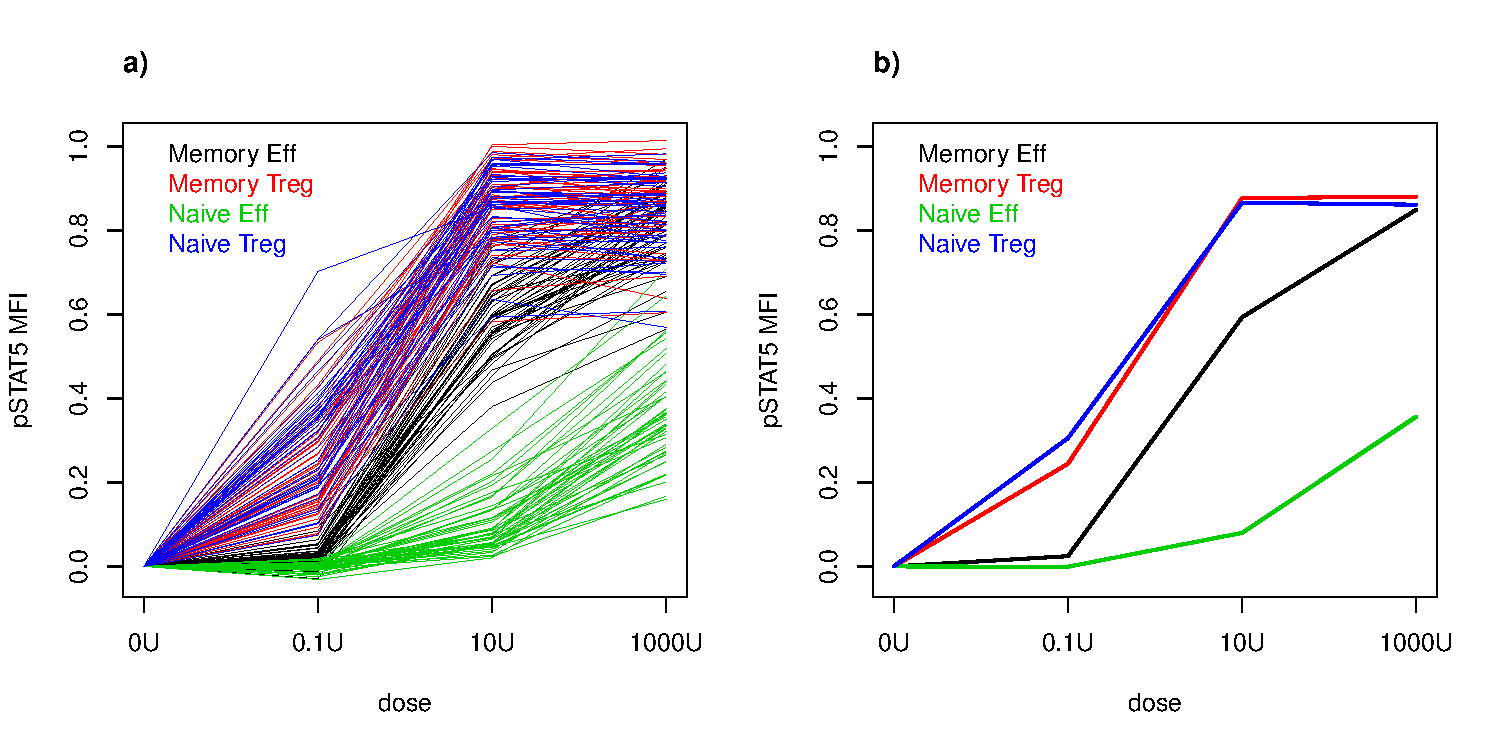
\includegraphics[scale=.5]{IL2/figures/pstat5-auc-celltypes.pdf}
    \mycaption{figure:pstat5-auc-celltypes}
    { pSTAT5 area under dose-response curve }
    { a) The dose-response curve for each cell type in all samples. b) The medians dose-response curve across all samples for each cell type.}
\end{figure}

\begin{figure}[h]
    \centering
    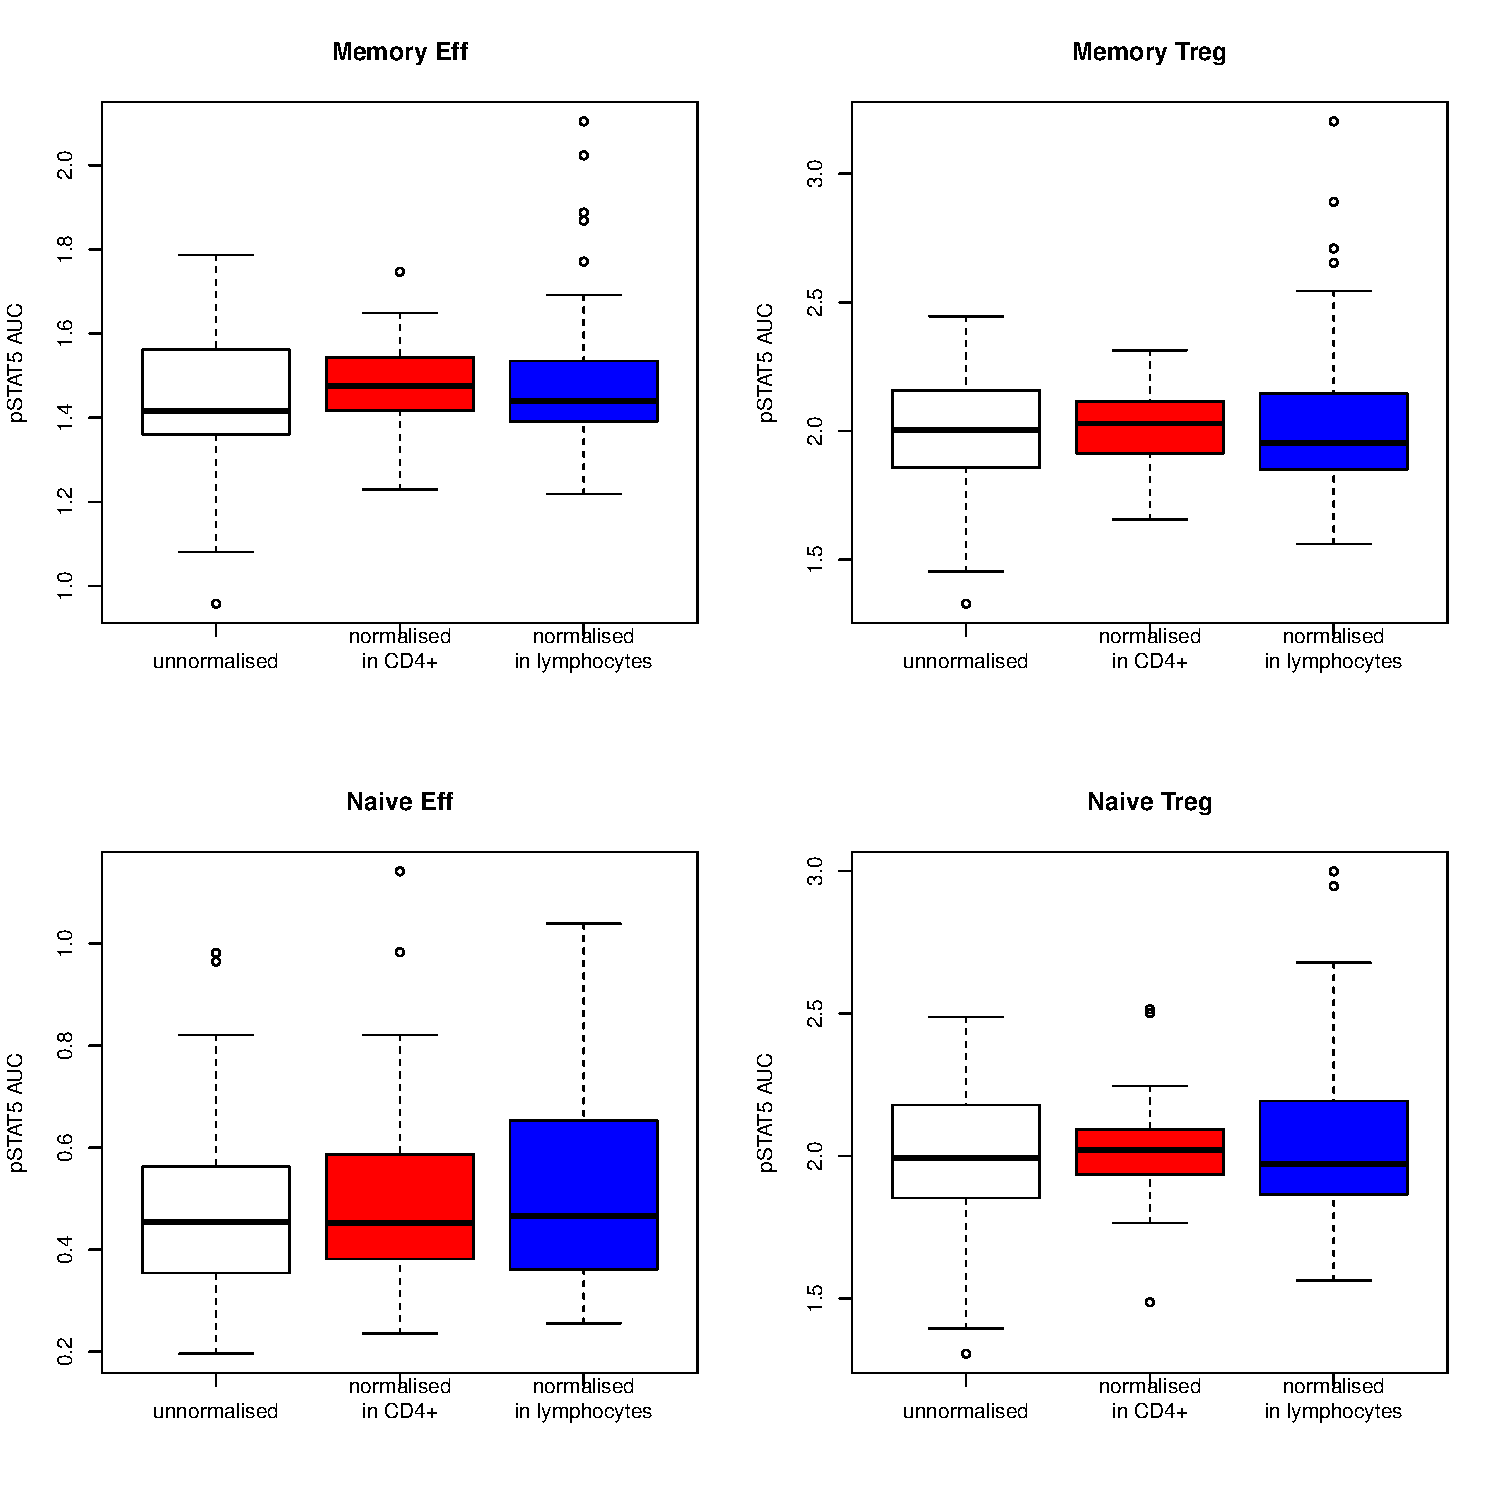
\includegraphics[scale=.5]{IL2/figures/pstat5-auc-boxplots-celltypes.pdf}
    \mycaption{figure:pstat5-auc-boxplots-celltypes}
    { Influence of normalisation method on pSTAT5 area under curve. }
    { In red the normalisation using the peak alignment in CD\positive lymphocytes, in blue the normalisation using peak alignment in lymphocytes. }
\end{figure}


\begin{figure}[h]
    \centering
    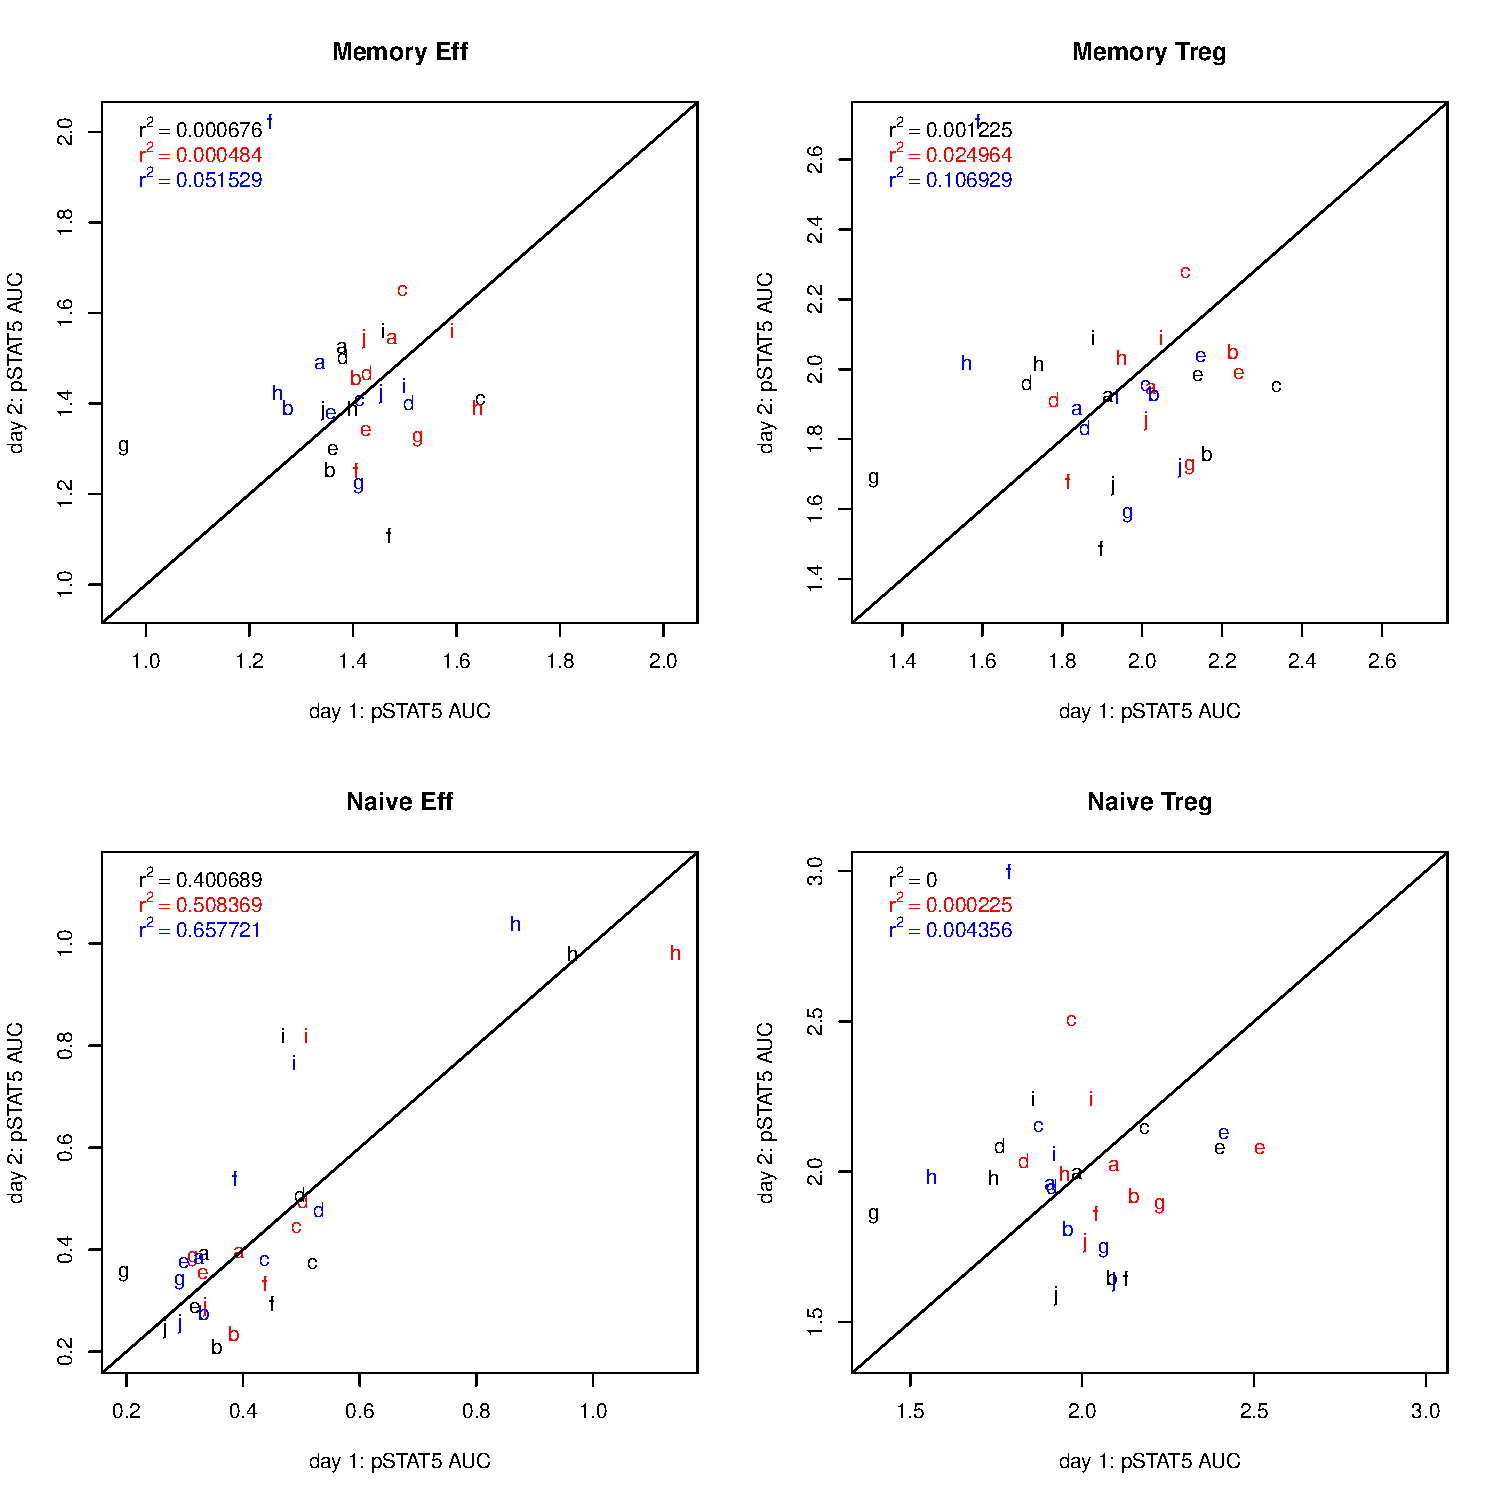
\includegraphics[scale=.5]{IL2/figures/pstat5-auc-repeatability-celltypes.pdf}
    \mycaption{figure:pstat5-auc-repeatability-celltypes}
    { Influence of normalisation on the repeatability of the pSTAT5 area under the curve. }
    { In red the normalisation using the peak alignment in CD\positive lymphocytes, in blue the normalisation using peak alignment in lymphocytes. }
\end{figure}


%In the manual analysis conducted by Tony Cutler, he found that he could identify individuals which were low or high responders.
%This leads us to hypothesise that within one individual the response to \emph{IL-2} on day 1 should be comparable to the response to \emph{IL-2} on day 2.

%One method we have tried is based on the assumption is that in the ungated data, the bottom and top percentile of the pSTAT5 distribution do not respond to \emph{IL-2} and so can be used as reference points.  This is effectively a quantile normalisation method aligning the bottom and top percentile across doses.

%However we found that this normalisation method d is not true in CD4+ lymphocyte gated data.


%Certain normalisation methods make assumptions about the shape of the data.
%The actual choice of normalisation depends on the characteristics of the data we wish to compare.
%Certain normalisation methods such as quantile normalisation are not appropriate since they assume the distributions have the shame shape.


%\begin{figure}[h]
%%
%%#simulated data
%%x0 <- mixtools::rnormmix(1000, mu=c(1,6), lambda=c(.3,.7))
%%x1 <- mixtools::rnormmix(1000, mu=.9*c(1,6)+2, lambda=c(.5,.5), sigma=c(2,2))
%%d0 <- density(x0)
%%d1 <- density(x1)
%%l0 <- extract.landmarks(x0,max.lms=2, bw=d0$bw)
%%l1 <- extract.landmarks(x1,max.lms=2, bw=d1$bw)
%%m <- lm(l0$lms ~ l1$lms)
%%x1.norm <- cbind(1,x1)%*%coefficients(m)
%%l1.norm <- extract.landmarks(x1.norm,max.lms=2)
%%#before align
%%pdf('~nikolas/GoogleDrive/PhD/Thesis/IL2/figures/simulation-peak-align-noise.pdf')
%%plot(d0,xlim=c(-3,11),main='', xlab='')
%%points(l0$lms, l0$dens, pch=20, cex=2)
%%lines(d1, lty=2)
%%points(l1$lms, l1$dens, pch=20, cex=2)
%%#after peak align
%%lines(density(x1.norm), lty=2, col='red')
%%points(l1.norm$lms, l1.norm$dens, pch=20, cex=2, col='red')
%%dev.off()
%%
    %\centering
    %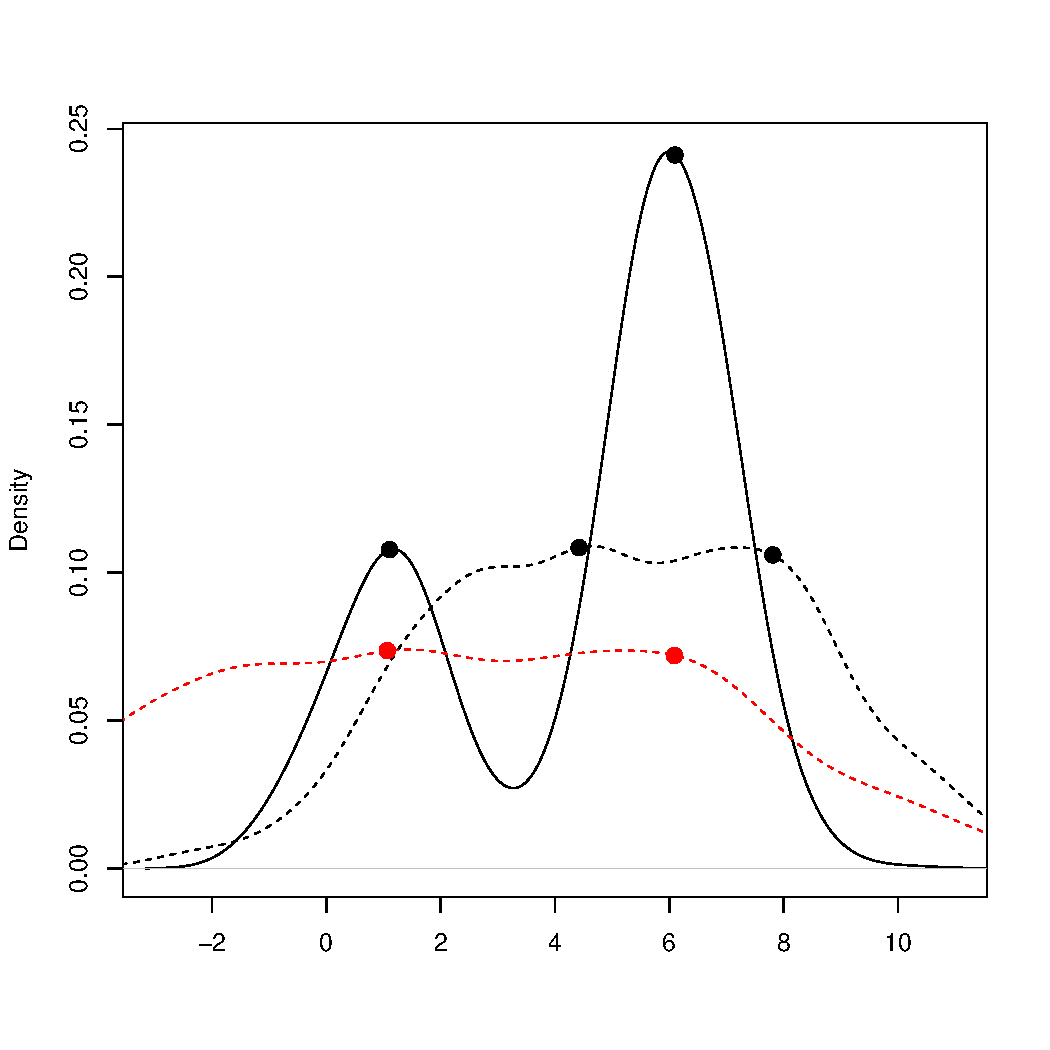
\includegraphics[scale=1]{IL2/figures/simulation-peak-align-noise.pdf}
    %\caption{  \label{figure:simulation-peak-align-noise}  In solid black line represents the density function obtained from $1000$ draws from a mixture of two normal distribution
    %with means $\mu_0=(1,6)$, standard deviations $\sigma_0=(1,1)$ and mixing proportions $\tau_0=(.3,.7)$.
    %The dashed black line represents the density function obtained from $1000$ draws from a mixture of two normal distribution
    %where $\mu_1 = 0.9 \mu_0 + 2$, standard deviations $\sigma_0=(1,1)$ and $\tau_1=(.5,.5)$.
    %The red dashed line represents the transformation using peak alignment. }
%\end{figure}
%

%%e <- lapply(flat.rep.fcs[names(flat.rep.fcs)[1:4]], function(x) ecdf(lgcl(getChannels(x, 'pstat5'))))
%%d <- lapply(flat.rep.fcs[names(flat.rep.fcs)[1:4]], function(x) density(lgcl(getChannels(x, 'pstat5')),bw=.1))
%%d.f <- lapply(d, function(d) splinefun(d$x,d$y))
%%y.max <- max(sapply(d, function(d) d$y)) 
%%e <- lapply(lymph[names(lymph)[1:4]], function(x) ecdf(lgcl(getChannels(x, 'pstat5'))))
%%d <- lapply(lymph[names(lymph)[1:4]], function(x) density(lgcl(getChannels(x, 'pstat5')),bw=.1))
%%d.f <- lapply(d, function(d) splinefun(d$x,d$y))
%%y.max <- max(sapply(d, function(d) d$y)) 
%%#pdf('~nikolas/lymph-dose-effect.pdf',width=10,height=5)
%%pdf('~nikolas/ungated-dose-effect.pdf',width=10,height=5)
%%par(mfrow=c(1,2))
%%x <- seq(-.5, 3, length.out=20000)
%%plot(x, e[[1]](x), col='white', xlab='pSTAT5', xlim=c(-.5,3), ylab='') 
%%mapply(function(e,lwd,lty) lines(x,e(x),lwd=lwd,lty=lty),e,seq(1,2.5,.5),c(1,2,2,1))
%%legend('topleft',doses, lwd=seq(1,2.5,.5), lty=c(1,2,2,1))
%%plot(x, d.f[[1]](x), col='white', xlab='pSTAT5', xlim=c(-.5,3),ylim=c(0,1),ylab='') 
%%mapply(function(d,lwd,lty) lines(x,d(x),lwd=lwd,lty=lty),d.f,seq(1,2.5,.5),c(1,2,2,1))
%%legend('topleft',doses, lwd=seq(1,2.5,.5), lty=c(1,2,2,1))
%%dev.off() 
%%pdf('~nikolas/ungated-lymph-dose-effect.pdf')
%%par(mfrow=c(1,1))
%%x <- seq(-.5, 3, length.out=20000)
%%plot(x, d.f[[1]](x), col='white', xlab='pSTAT5', xlim=c(-.5,3),ylim=c(0,1),ylab='') 
%%d <- lapply(flat.rep.fcs[names(flat.rep.fcs)[c(1,4)]], function(x) density(lgcl(getChannels(x, 'pstat5')),bw=.1))
%%d.f <- lapply(d, function(d) splinefun(d$x,d$y))
%%y.max <- max(sapply(d, function(d) d$y))
%%mapply(function(d,lwd,lty) lines(x,d(x),lwd=lwd,lty=lty),d.f,c(1,2.5),1)
%%d <- lapply(lymph[names(lymph)[c(1,4)]], function(x) density(lgcl(getChannels(x, 'pstat5')),bw=.1))
%%d.f <- lapply(d, function(d) splinefun(d$x,d$y))
%%y.max <- max(sapply(d, function(d) d$y))
%%#r <- mapply(function(a,b) length(a)/length(b), lymph[1:4], flat.rep.fcs[1:4])
%%mapply(function(d,lwd,lty) lines(x,d(x),lwd=lwd,lty=lty,col='red'),d.f,c(1,2.5),1) 
%%legend('topleft',doses[c(1,4)], lwd=c(1,2.5), lty=1)
%%dev.off()
%%lymph <- sapply(flat.rep.fcs, function(x) { cd4 <- lgcl(getChannels(x, 'cd4')); return(x[2 <  cd4 & cd4 < 2.75,]) })
%%

\subsection{Association of pSTAT5 response with type 1 diabetes}

Having improved the reproducibility of the cell phenotype with normalisation via peak alignment, we are now in a position to test
the original hypothesis of whether type 1 diabetics show a reduced response to proleukin in those cell subsets.
We account for repeated individuals with a linear mixed effects model as applied in Chapter 2.%\Cref{chapter:il2ra}.

Having not identified a significant association, this now brings us to the next question of whether there are other
cell subsets besides the ones which we are gating which are sensitive to proleukin, and in particular low doses of proleukin?


\begin{figure}[h]
    \centering
    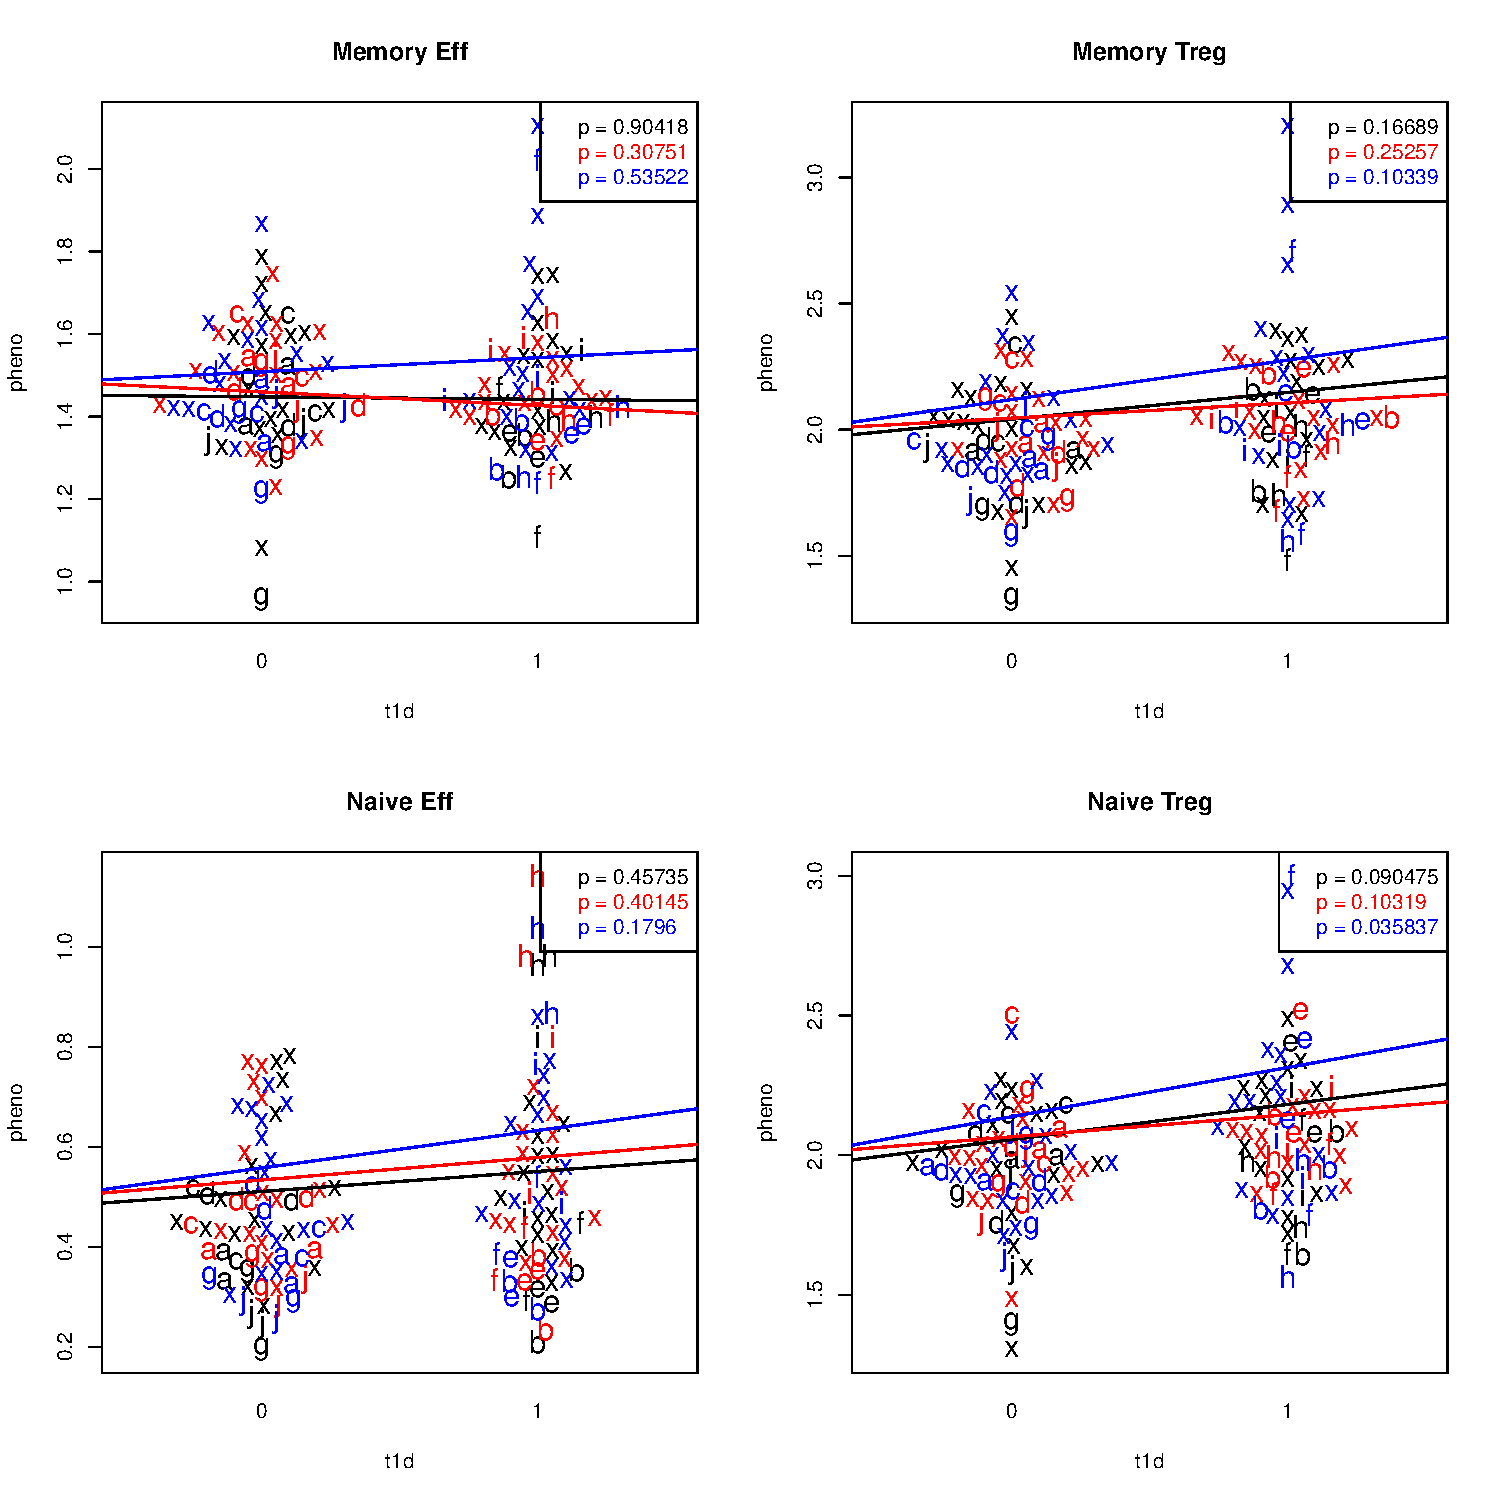
\includegraphics[scale=.5]{IL2/figures/pstat5-auc-t1d-celltypes.pdf}
    \mycaption{figure:pstat5-auc-t1d-celltypes}
    { Influence of normalisation on the association of pSTAT5 area under the curve with type 1 diabetes in the four cell subsets. }
    { }
\end{figure}



\section{Response in the whole sample}

%\begin{figure}[h]
    %\centering
    %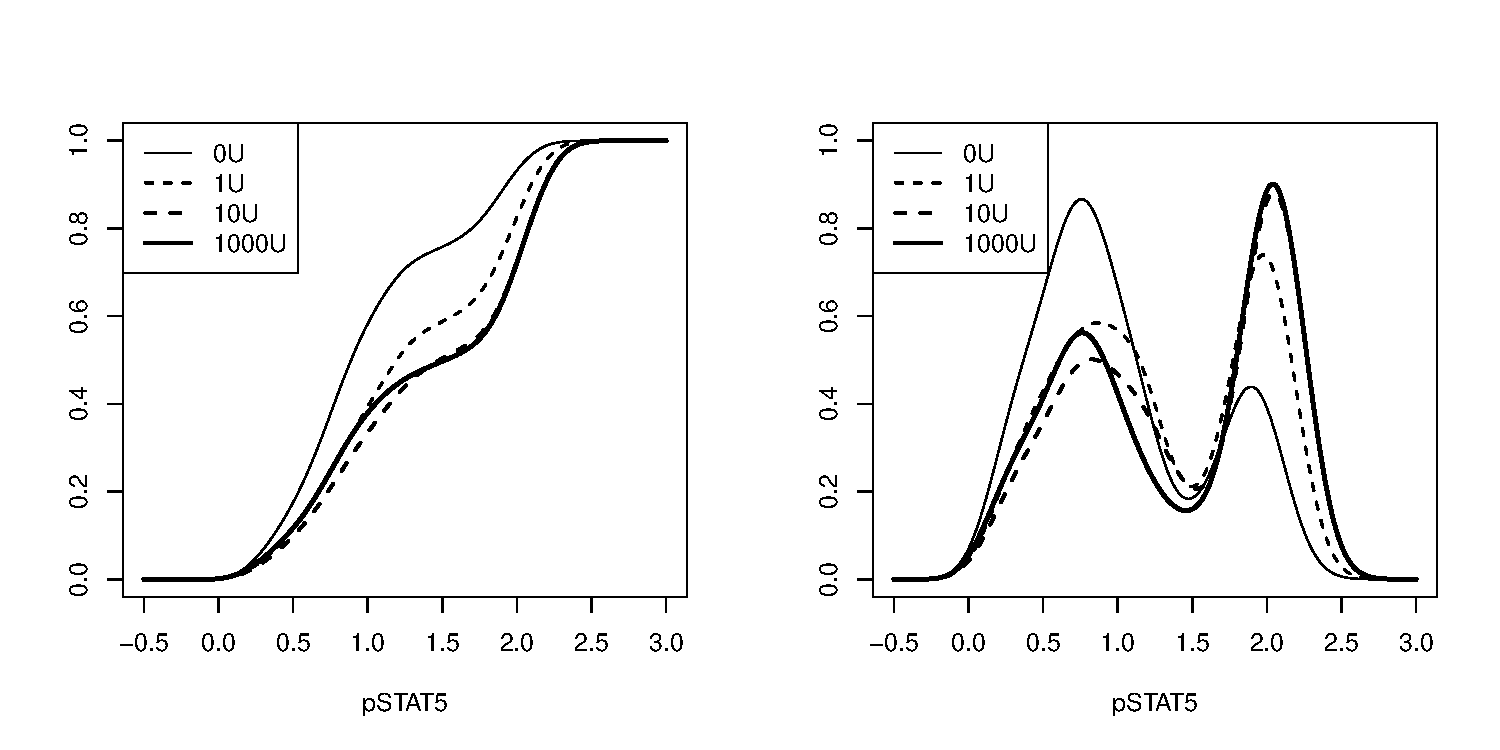
\includegraphics[scale=.5]{IL2/figures/ungated-dose-effect.pdf}
    %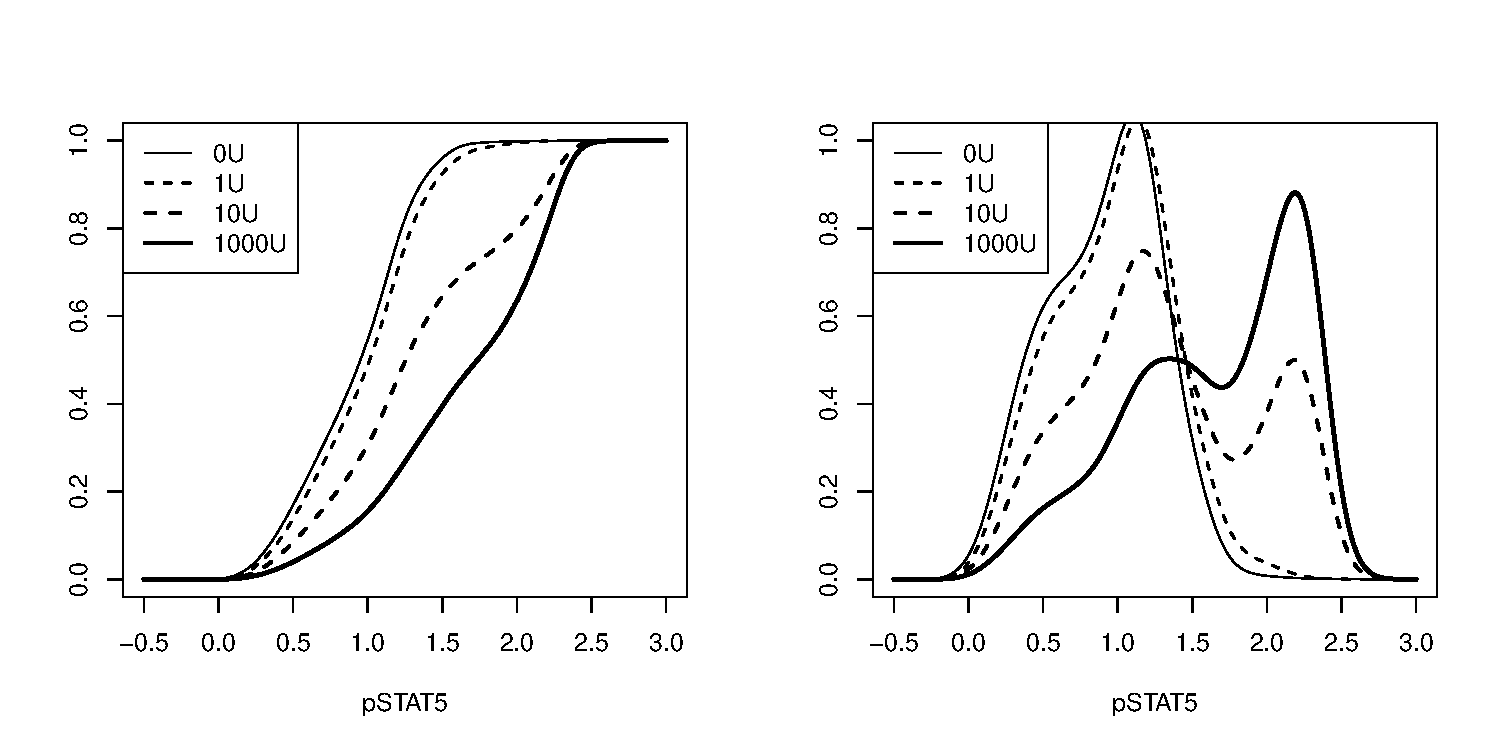
\includegraphics[scale=.5]{IL2/figures/lymph-dose-effect.pdf}
    %\mycaption{figure:dose-effect}
    %{Dose effect.}
    %{
        %On the left the cumulative density function obtained from individual a on day 1 across 4 increasing doses.
        %On the right the density function.
        %The top two figures are from the ungated sample.
        %The bottom two figures are from a CD4 range gate.
        %We observe that in the unstimulated sample the distribution is already bimodal 
        %and that upon stimulation the location of the peaks does not change much but that the height changes greatly.
        %Contrary to the ungated data, the pSTAT5 distribution in the CD4 gated sample now appears unimodal when resting or stimulated
        %at the lowest 1U dose.  At the higher doses we start seeing a bimodal distribution.
        %In the ungated sample, the location of the activation peak seems to align somewhat with that of the activation peak.  }
%\end{figure}
%


%In \Cref{figure:dose-effect} we observe that at the lowest 0.1U dose there seems to be a much more stronger relative repsonse
%in the whole sample than in the lymphocyte subset which suggests that there exist other cells beside CD4\positive lymphocytes
%which are also responsive to low doses of IL-2.  
%However the relative difference in response between 10U and 1000U seems much more important in lymphocytes than in the whole sample
%suggesting that the non-CD4\positive lymphocytes in the whole sample reach saturation at 0.1U.
%Also since the resting sample sample displays a shoulder this suggests a mixture of resting and already semi-activated lymphocytes.

We are interested in identifying and classifying cell subsets by their sensitivity to proleukin.  
When assessing the dose-response to stimulation in a flow cytometry sample,
the classic approach is to gate cell populations in each sample based on their core markers,
and then assess the response of the functional marker in gated subset.
This approach however, may miss other dose-responsive cell populations which are not included in the gating.

%While the manual gating inspired approach is the established method, it suffers from a major drawback:
%it relies on prior knowledge of the number of cell populations and consequently misses the pSTAT5 response in uncharacterised cell subsets.

\subsection{Visualising response in whole sample with SPADE}

Methods like SPADE can give us an overview of the dose-response in the whole sample in the form of a \gls{MST}.
%The visualisation requires downsampling requires downsampling.
However, the generated minimum spanning tree requires some annotation in order to understand where lie the different cell types.
I also found that the mapping of the manual gates to the MST was not intuitive.
As can be seen in \Cref{figure:spade-celltypes}, cell types defined by the manual gates are spread across different branches of the tree
and different cell types map to the same nodes.
Furthermore, SPADE requires pooling across samples for comparison of the \gls{MST}, which is not adviseable given that the core
markers are not stable across days.

\hspace{-2cm}
\begin{figure}[h]
  \centering
\begin{subfigure}[b]{.4\textwidth}
  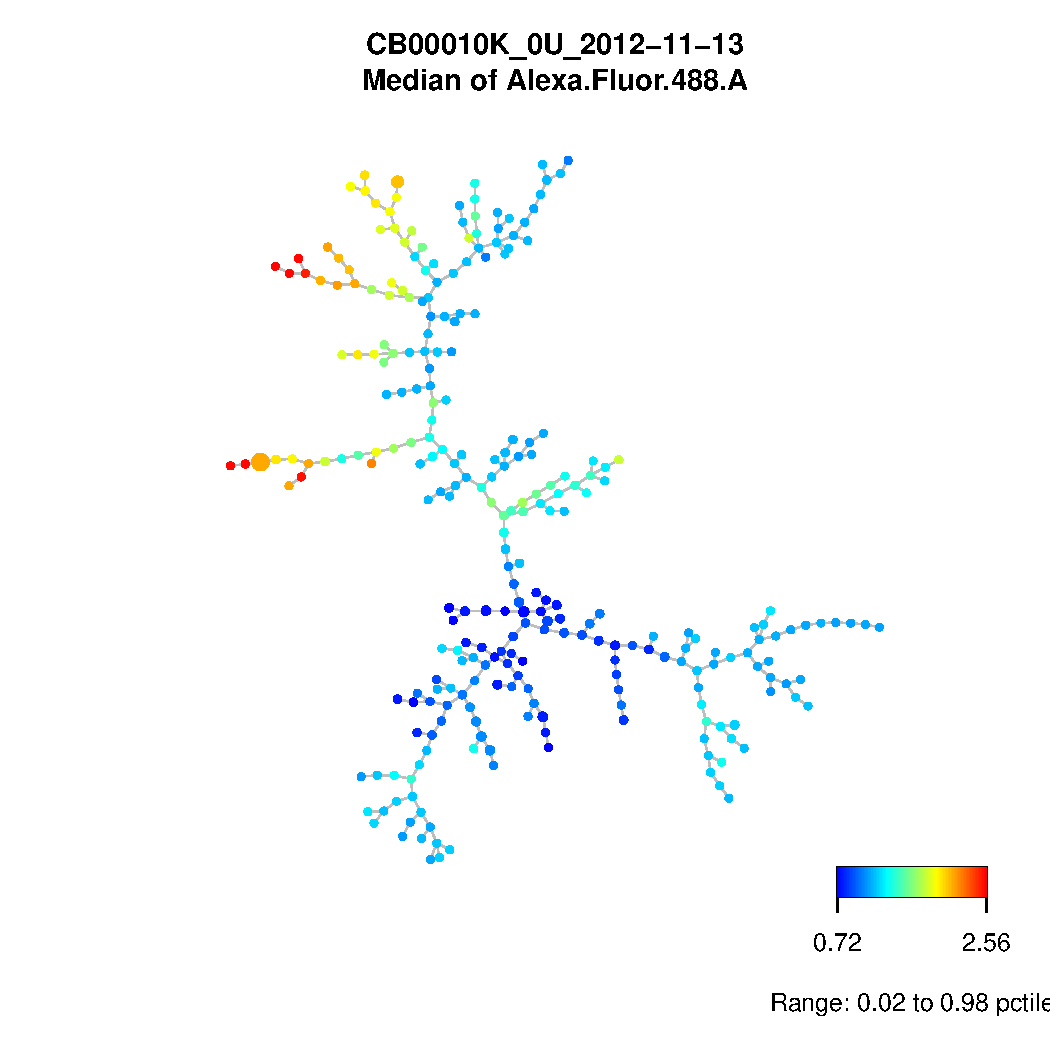
\includegraphics[scale=.4]{IL2/figures/CB00010K-0U-2012-11-13-spade.pdf}
\caption{Resting sample.}
\end{subfigure}
\begin{subfigure}[b]{.4\textwidth}
  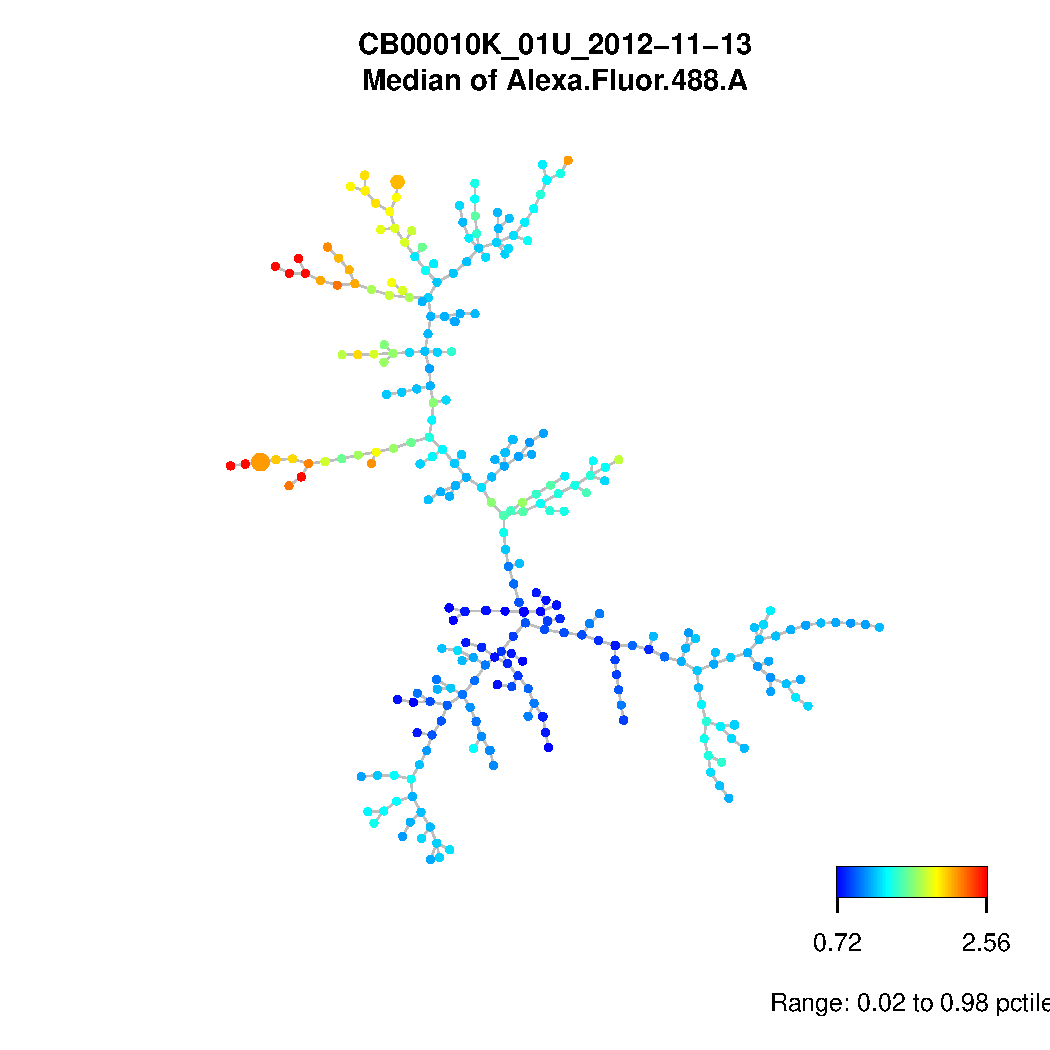
\includegraphics[scale=.4]{IL2/figures/CB00010K-01U-2012-11-13-spade.pdf}
  \caption{0.1 units}
\end{subfigure}
\begin{subfigure}[b]{.4\textwidth}
  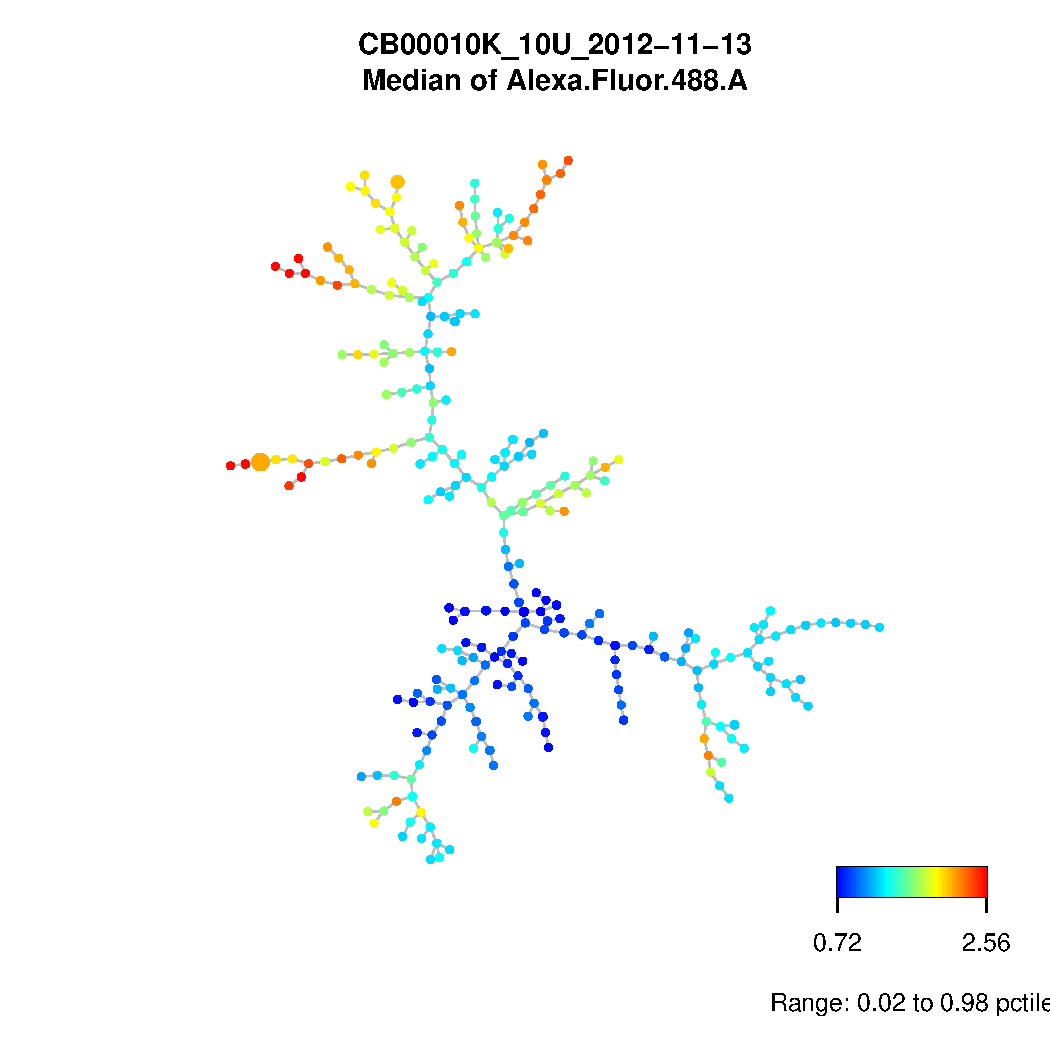
\includegraphics[scale=.4]{IL2/figures/CB00010K-10U-2012-11-13-spade.pdf}
  \caption{10 units}
\end{subfigure}
\begin{subfigure}[b]{.4\textwidth}
  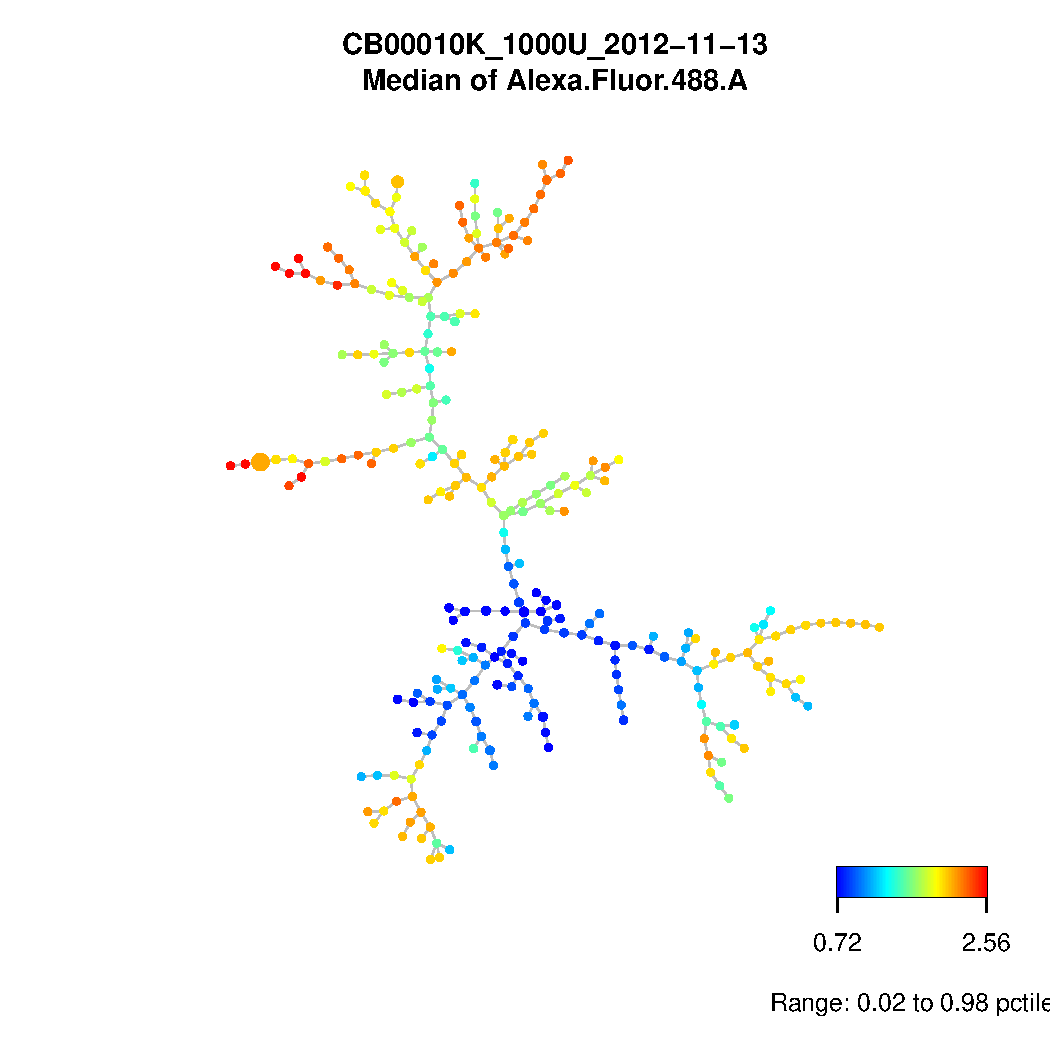
\includegraphics[scale=.4]{IL2/figures/CB00010K-1000U-2012-11-13-spade.pdf}
  \caption{1000 units}
\end{subfigure}
    \mycaption{figure:spade-ouput}
    {SPADE output on sample.}
    {
    }
\end{figure}



\begin{figure}[h]
    \centering
    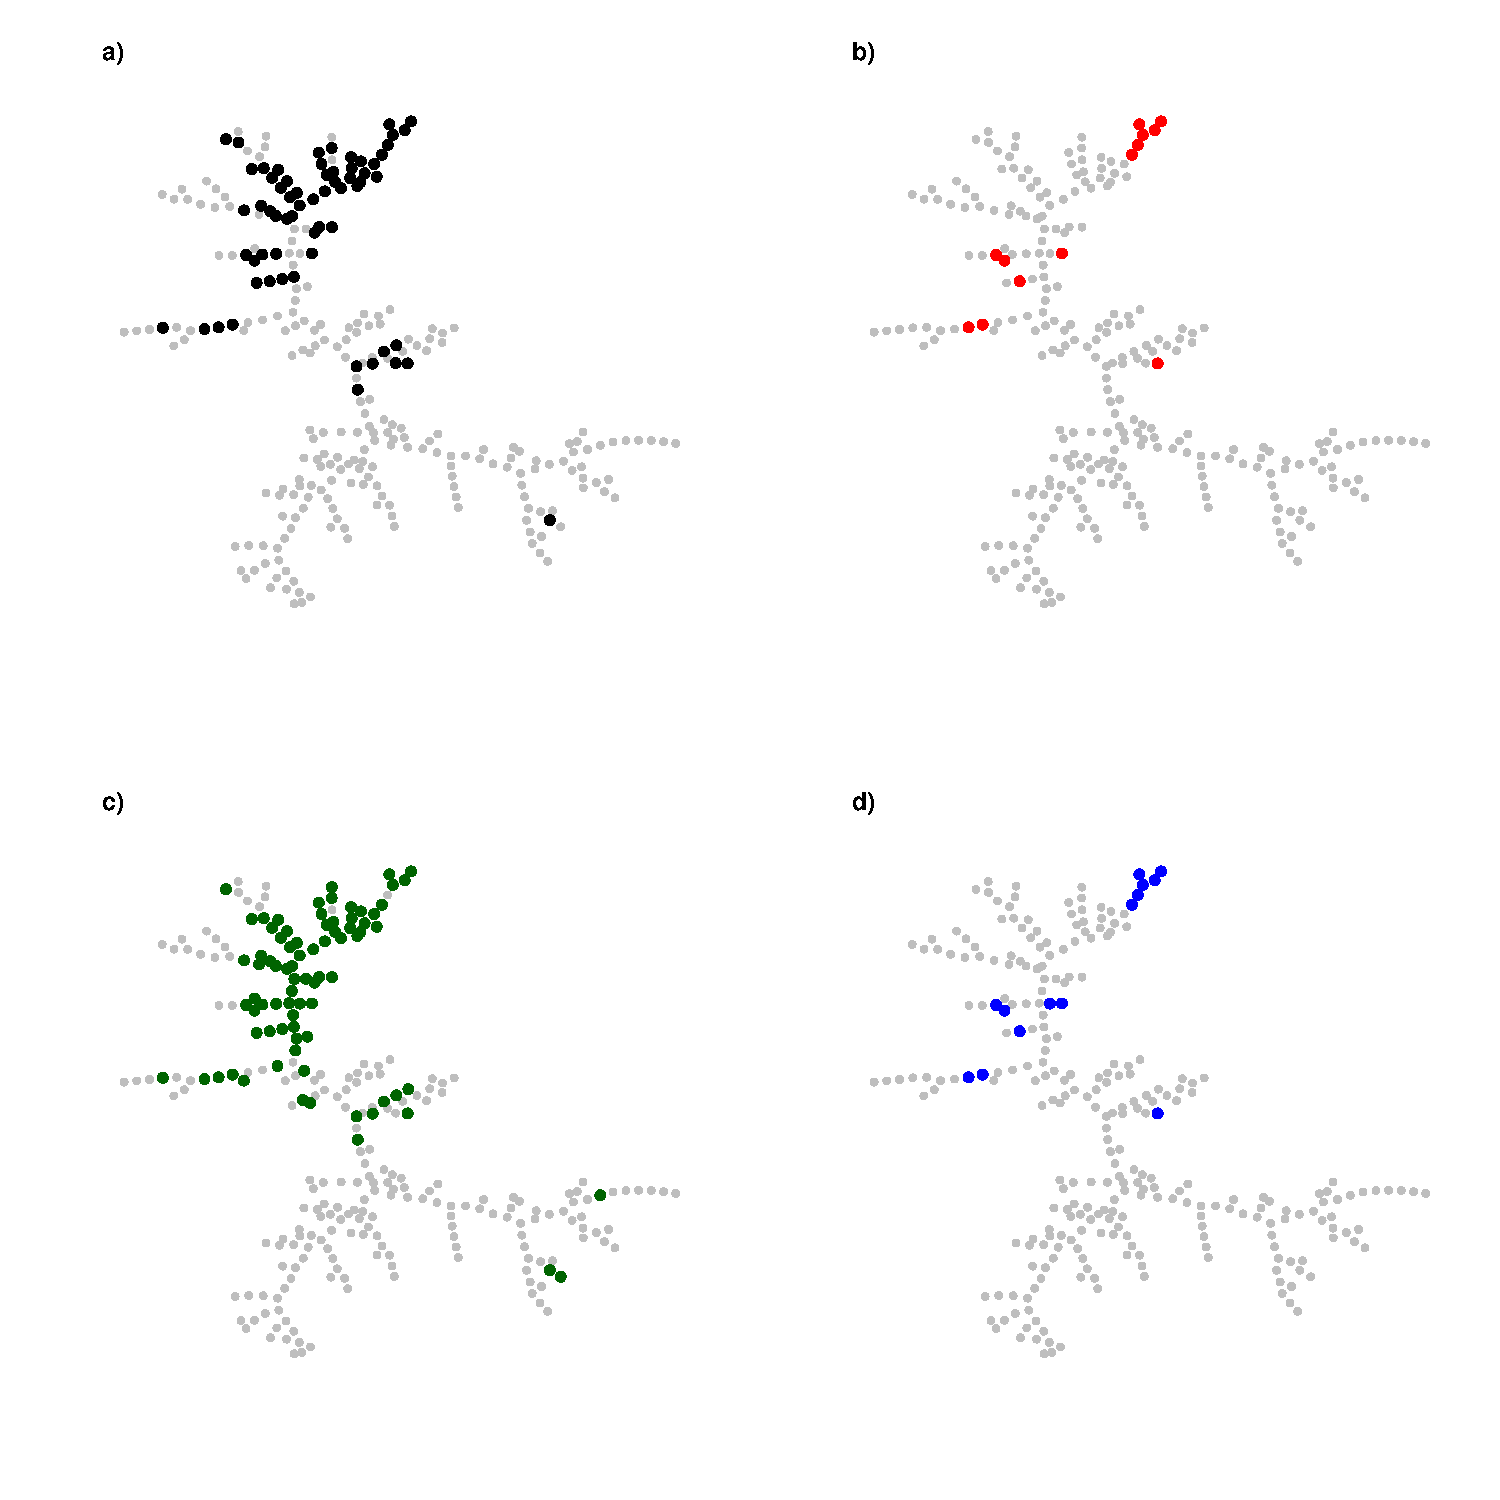
\includegraphics[scale=.5]{IL2/figures/spade-celltypes.pdf}
    \mycaption{figure:spade-celltypes}
    {Mapping of cell types defined by manual gates to SPADE tree.}
    {
      Memory effectors (a), memory regulatory T cells (b), naive effectors (c) and naive regulatory T cells (d), overlap which complicates
      the interpretation.
    }
\end{figure}



\subsection{Prediction of pSTAT5 response with Random Forests}

I found that using methods like \gls{RF} and \gls{MARS}, I could approximate the pSTAT5 response with a multivariate non-linear function.
This could be useful for predicting the pSTAT5 response from only core marker information.
However, here we seek an interpretable model which can be summarised as rules to identify groups of cells which are sensitive to proleukin.
Ideally, we would like to identify cells types which are unimodal on pSTAT5 (like the naive and memory T regs) through proleukin doses,
although these cells may not necessarily be unimodal on the other markers.
%and contain more than N points.
%Need to give more weight to pSTAT5 in clustering.

%It has been hypothesised that certain lymphocyte subsets are less responsive to \cytokine{IL-2} stimulation in type 1 diabetics than in healthy controls.

%How many cell pops are they?


\subsection{Recursive partitioning of pSTAT5 response with classification and regression trees} 

%This yields a baseline relative response per cell which provides additional information which can be used in the gating.  
%Here I suggest another approach of identifying responsive cells by recursive partitioning on the core marker space with a \gls{CART} on the pSTAT5 response.
On method could be to use \gls{CART} so that the variance in the pSTAT5 response is use to guide the partitioning on the core markers.
The \gls{CART} considers each core marker individually and considers each core marker coordinate as a splitting point.
The splitting point which maximises the between class variance is selected over all markers and all values.
%the information gain of splitting at each value of that dimension.
%Considering the response in all cells, 

%Classification and regression trees are the most interpretable but risk overfitting the data and may not generalise to other samples.
%However here, overfitting is not a concern as provided cells can be identified in each sample individually which can then be checked by a human.




\hspace{-2cm}
\begin{figure}[h]
\centering
%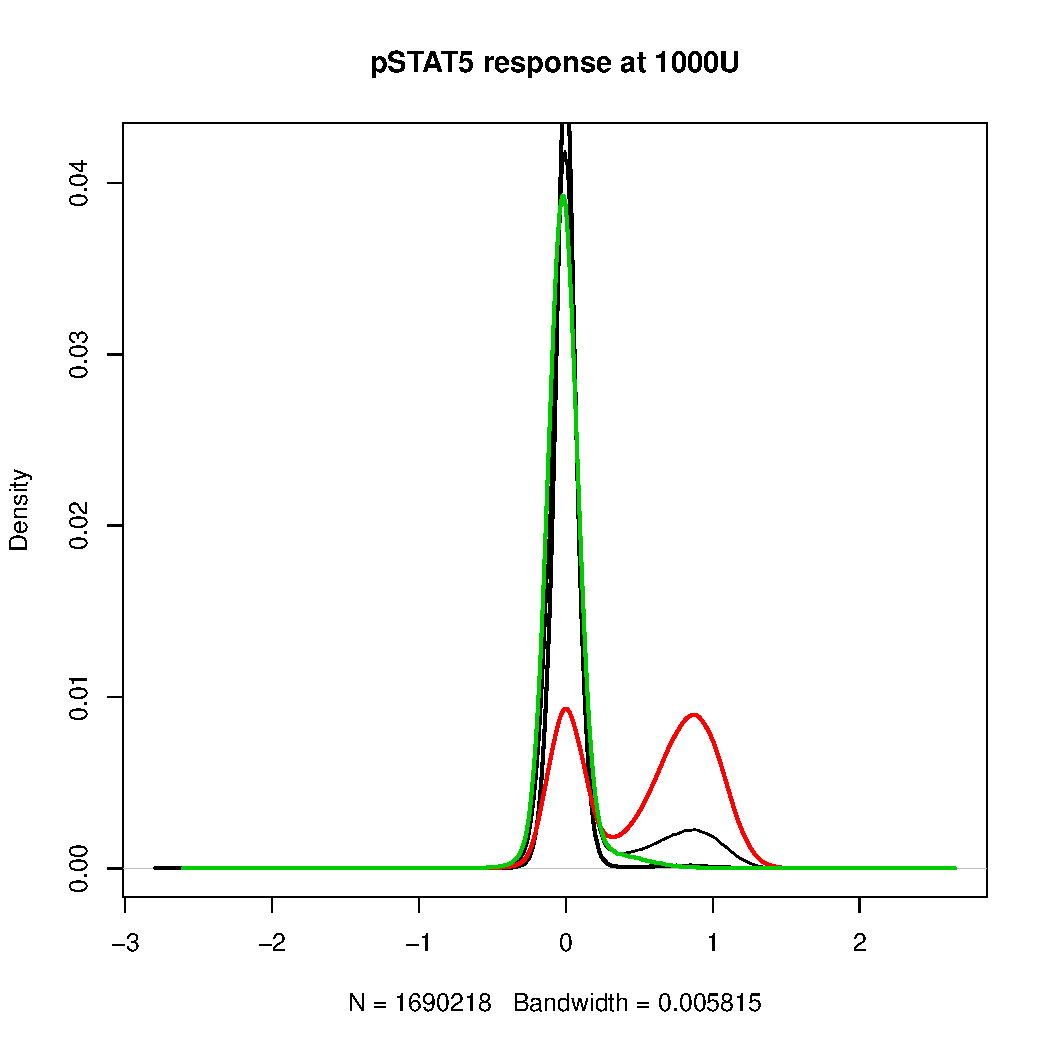
\includegraphics[scale=.45]{figures/pstat5-response-decision-tree-b.pdf}
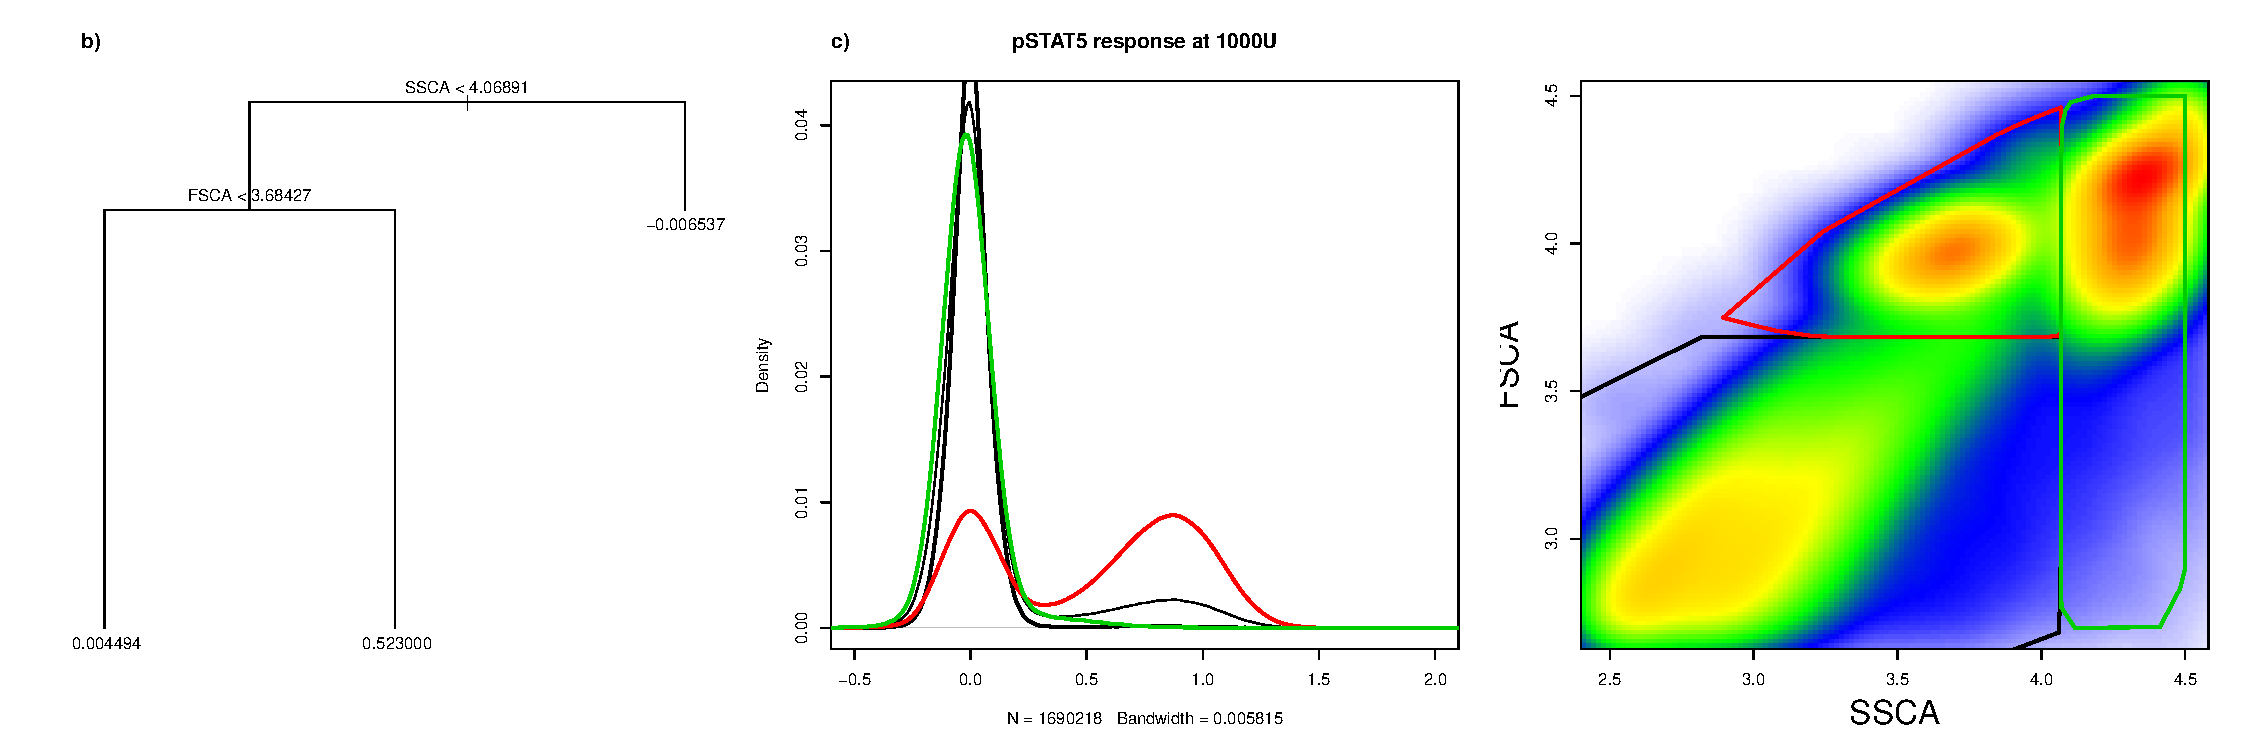
\includegraphics[scale=.45]{IL2/figures/pstat5-response-decision-tree.pdf}
\mycaption{figure:pstat5-response-decision-tree}
{ \gls{CART} on side and forward scatter identifies three subsets. }
{
Running classification tree on SSCA and FSCA, shows most of the pSTAT5 response comes from within the lymphocyte cluster (red) whereas
the black and green cluster are not as responsive.
The nice thing here is is that the recursive partitioning of pSTAT5 corresponds to the clustering of SSCA and FSCA.
}
\end{figure}


\subsection{Identification of highly sensitive cells with recursive partitioning using two component mixture model}

Here I suggest another approach based on the idea that by recursively identifying the highest responding cells at decreasing doses, it should be
possible to drill down to the cells which respond to the lowest dose proleukin.
%As at the highest dose of proleukin, 1000 units, the pSTAT5 distribution appears bimodal, while at lower doses the response peak is less discernable.
%In the ungated sample the majority of cells are non-responsive even at the highest dose.
As illustrated in \Cref{figure:pstat5-rpart}, cells are divided as low responders and high responders on pSTAT5 response at 1000U 
within responders, and then further divided on low/high on pSTAT5 response at 10U.
This is repeated on pSTAT5 response at 0.1U.
Cells which consistently appear the high group are the most sensitive.
This hierarchical approach draws some similarity to the recursive partitioning using \gls{CART} except that the splitting is done using a two-component mixture model.
Also, at each step, the pSTAT5 at a lower dose is considered to discover cells which respond to the lowest dose of proleukin.

We find that, while many of the cells identified using this approach fall within the CD4 gate,
certain highly-sensitive cells cluster in other subsets \Cref{figure:new-cell-subset}.
Excluding doublets on the basis of side scatter width,
and examining the remainder on other channels these cells appear to be monocytes (from discussion with \contributor{Marcin Pekalski} and \contributor{Tony Cutler}),
although additional markers would be required to better characterise these cells.
Importantly, these cells would have been missed by manual gating since they are not lymphocytes.


\hspace{-2cm}
\begin{figure}[h]
\centering
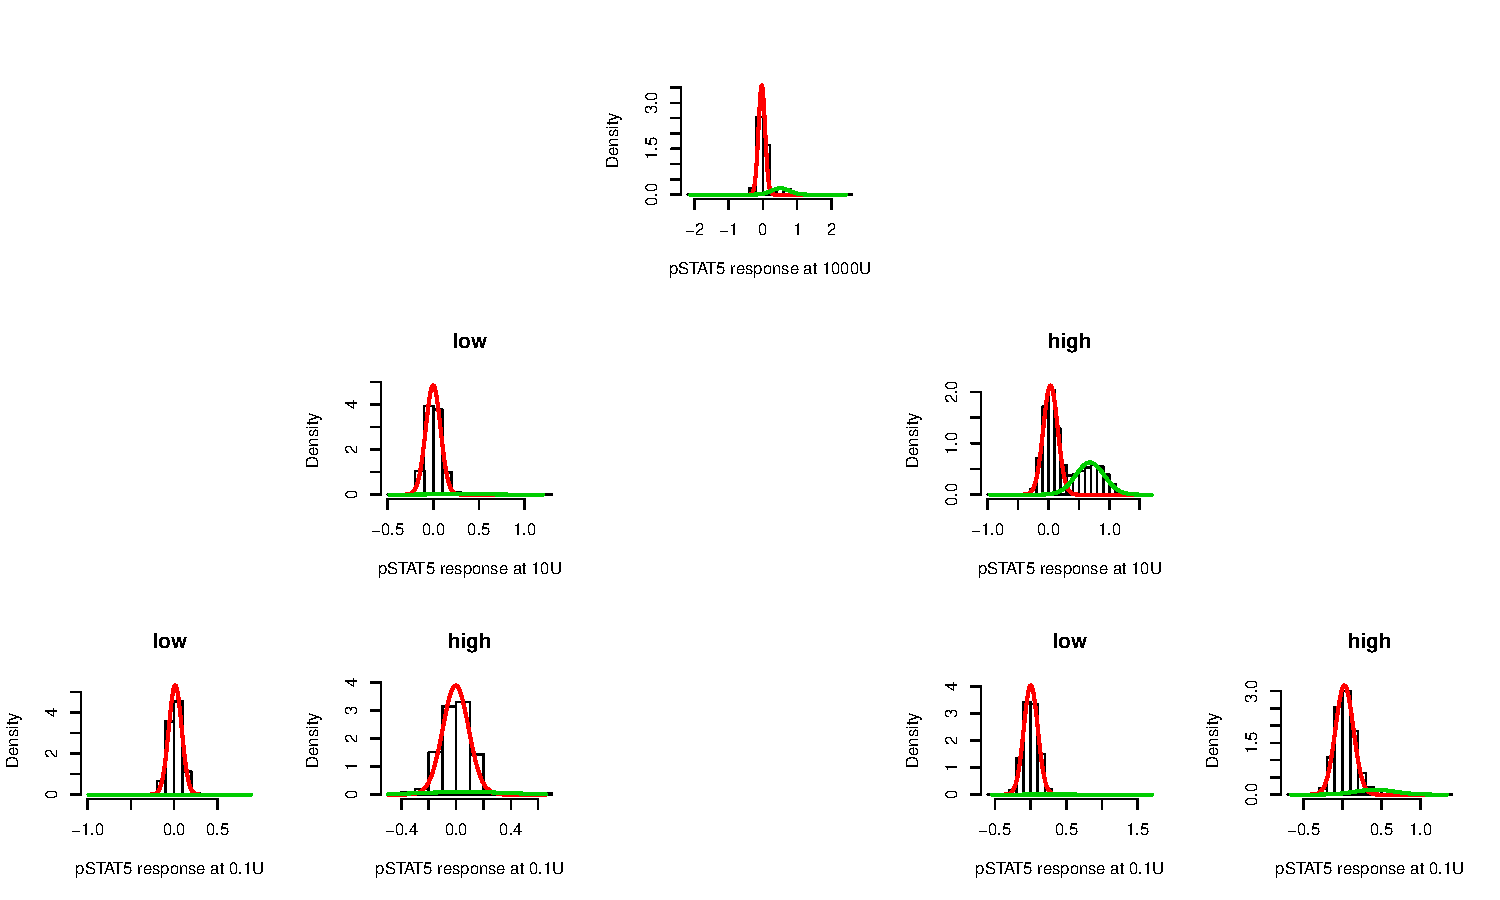
\includegraphics[scale=.5]{IL2/figures/pstat5-rpart.pdf}
\mycaption{figure:pstat5-rpart}
{ Recursive partitioning of pSTAT5 response into low and high populations to identify cells responsive to the lowest dose of proleukin. }
{
In the ungated sample the majority of cells are none responsive even at the highest dose.
Cells are divided as low responders and high responders on pSTAT5 response (i.e baseline subtracted) at 1000U 
within responders further divide on low/high on pSTAT5 response at 10U
repeat on pSTAT5 response at 0.1U
cluster ones which are consistently high, these are the most sensitive cell populations 
}
\end{figure}


\hspace{-2cm}
\begin{figure}[h]
\centering
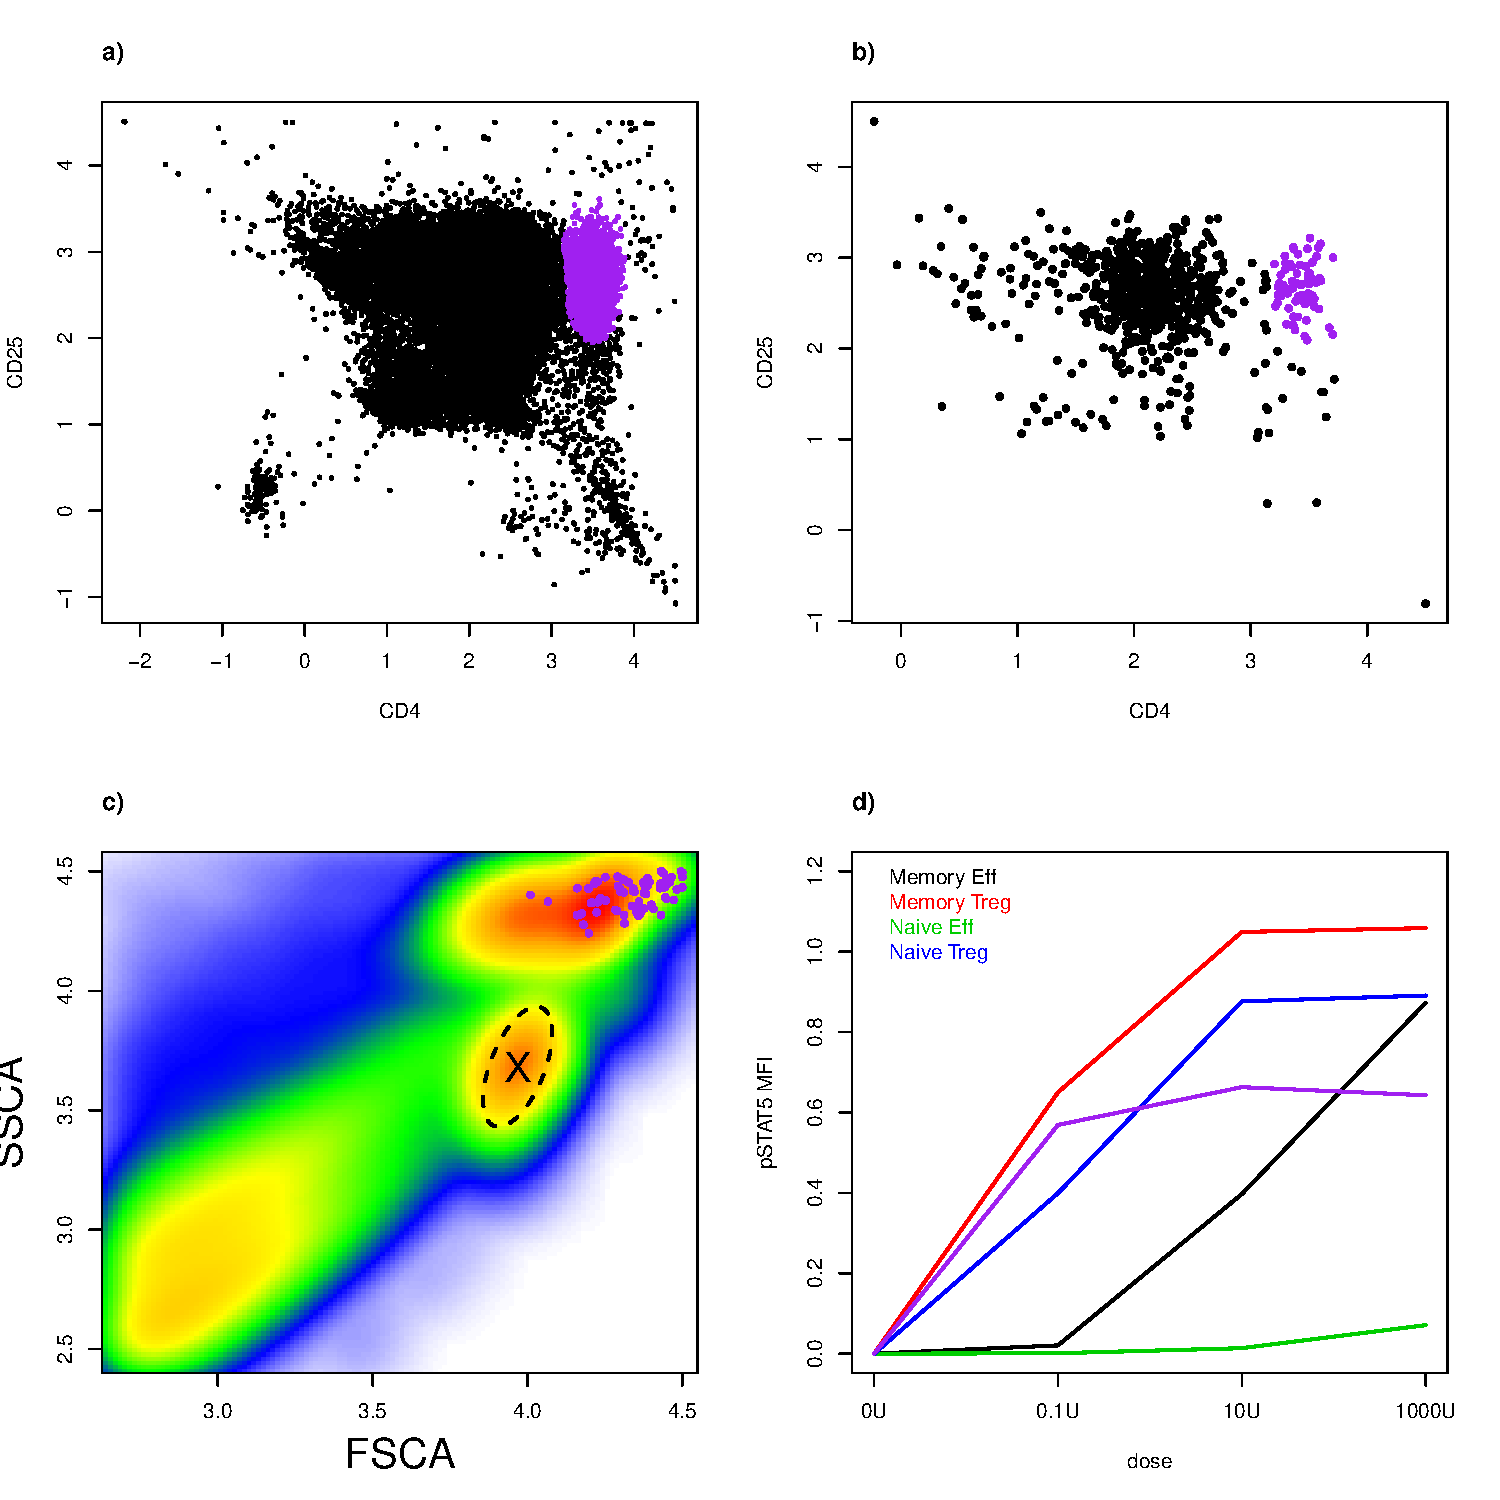
\includegraphics[scale=.5]{IL2/figures/new-cell-subset.pdf}
\mycaption{figure:new-cell-subset}
{ Identification of low-dose sensitive non-CD4\positive lymphocyte population through recursive partitioning of pSTAT5 response. }
{
  By pooling all high-responsive cells on CD4 and CD25 , we identify a cluster of cells high on CD4 (a).
  This cluster of cells is identifiable in a single sample (b).
  According to forward and side scatter, these cells are unlikely to be lymphocytes (c).
  These cells show high-sensitivity to low-doses of proleukin but rapidly reach saturation (d).
  This is probably because they have high resting pSTAT5 levels.
  
}
\end{figure}





